% Rapport du Mini-Projet 17 — compiler depuis le dossier rapport/ avec :
%   tectonic rapport.tex
% Les graphiques de données (figures/*.pdf) se régénèrent avec :
%   docker compose run ... dashboard python rapport/exporter_donnees.py   (données du lakehouse)
%   py -3.10 rapport/generer_figures.py                                    (graphiques)
\documentclass[11pt,a4paper]{report}

\usepackage[french]{babel}
\usepackage{fontspec}
% Open Sans (fournie avec TeX) pour les titres et les schémas : très proche de
% Segoe UI, utilisée par les graphiques Matplotlib.
\setsansfont{OpenSans}[Extension=.ttf, UprightFont=*-Regular, BoldFont=*-Bold,
  ItalicFont=*-Italic, BoldItalicFont=*-BoldItalic, FontFace={sb}{n}{*-SemiBold}]
\usepackage{geometry}
\geometry{top=2.5cm,bottom=2.5cm,left=2.6cm,right=2.4cm,headheight=14pt}
\usepackage[table]{xcolor}
\usepackage{graphicx}
\usepackage{booktabs}
\usepackage{array}
\usepackage{amsmath}
\usepackage{enumitem}
\usepackage{multicol}
\usepackage{tikz}
\usetikzlibrary{arrows.meta,positioning,calc,shapes.geometric,decorations.pathreplacing,fit,backgrounds}
\usepackage{tcolorbox}
\usepackage{listings}
\usepackage{fancyhdr}
\usepackage{titlesec}
\usepackage{caption}
\usepackage{newunicodechar}
\newunicodechar{→}{\ensuremath{\rightarrow}}
\newunicodechar{≈}{\ensuremath{\approx}}
\usepackage[colorlinks=true,linkcolor=blue!50!black,urlcolor=blue!50!black,
            citecolor=blue!50!black]{hyperref}

% ------- Couleurs (mêmes que les graphiques Matplotlib) -------
\definecolor{bleuprojet}{HTML}{2A78D6}
\definecolor{bleuclair}{HTML}{DCEAFB}
\definecolor{orangeprojet}{HTML}{EB6834}
\definecolor{orangeclair}{HTML}{FCE3D8}
\definecolor{grisclair}{HTML}{F4F4F1}
\definecolor{grisligne}{HTML}{E1E0D9}
\definecolor{grismoyen}{HTML}{A9A8A1}
\definecolor{vertcode}{HTML}{2E7D5B}
\definecolor{vertclair}{HTML}{DDF0E6}
\definecolor{encre}{HTML}{0B0B0B}
\definecolor{encre2}{HTML}{52514E}
% palette catégorielle des typologies (ordre fixe, cf. fraud/viz.py)
\definecolor{cat1}{HTML}{2A78D6}
\definecolor{cat2}{HTML}{EB6834}
\definecolor{cat3}{HTML}{1BAF7A}
\definecolor{cat4}{HTML}{EDA100}
\definecolor{cat5}{HTML}{E87BA4}
\definecolor{cat6}{HTML}{008300}
\definecolor{critique}{HTML}{D03B3B}

% ------- Informations à personnaliser -------
\newcommand{\etudiant}{Majd Saidi}
\newcommand{\enseignant}{[Nom de l'enseignant]}
\newcommand{\datesoutenance}{[Date de soutenance]}
\newcommand{\anneeuniv}{2026--2027}

% ------- Icônes (police Font Awesome 5 Free, fournie avec TeX) -------
\DeclareFontFamily{TU}{iconesfa}{}
\DeclareFontShape{TU}{iconesfa}{m}{n}{<-> \UnicodeFontFile{FontAwesome5Free-Solid-900.otf}{}}{}
\newcommand{\ico}[1]{{\usefont{TU}{iconesfa}{m}{n}\symbol{"#1}}}
\newcommand{\oui}{{\color{vertcode}\ico{F00C}}}
\newcommand{\non}{{\color{orangeprojet}\ico{F00D}}}
\newcommand{\partiel}{{\color{encre2}\ico{F042}}}

% ------- Titres -------
\titleformat{\chapter}[display]
  {\sffamily\color{encre}}
  {\fontseries{sb}\selectfont\large\color{bleuprojet}\chaptertitlename~\thechapter}
  {1pt}{\bfseries\LARGE}[\vspace{2pt}{\color{bleuprojet}\titlerule[1pt]}]
\titleformat{name=\chapter,numberless}[display]
  {\sffamily\color{encre}}{}{0pt}{\bfseries\LARGE}
  [\vspace{2pt}{\color{bleuprojet}\titlerule[1pt]}]
\titlespacing*{\chapter}{0pt}{-14pt}{14pt}
\titleformat{\section}{\sffamily\bfseries\large}{\color{bleuprojet}\thesection}{0.6em}{}
\titlespacing*{\section}{0pt}{12pt plus 3pt minus 2pt}{5pt plus 1pt}
\titleformat{\subsection}{\sffamily\bfseries}{\color{bleuprojet}\thesubsection}{0.6em}{}
\titlespacing*{\subsection}{0pt}{9pt plus 2pt minus 2pt}{3pt plus 1pt}
\renewcommand{\chaptermark}[1]{\markboth{\thechapter.\ #1}{}}

% ------- En-têtes et pieds de page -------
\pagestyle{fancy}
\fancyhf{}
\renewcommand{\headrulewidth}{0.4pt}
\fancyhead[L]{\small\sffamily\color{encre2}\nouppercase{\leftmark}}
\fancyhead[R]{\small\sffamily\thepage}
\fancypagestyle{plain}{\fancyhf{}\renewcommand{\headrulewidth}{0pt}
  \fancyfoot[C]{\small\sffamily\thepage}}

% ------- Légendes, flottants, listes -------
\DeclareCaptionFont{bleu}{\color{bleuprojet}}
\captionsetup{font=small, labelfont={bf,sf,bleu}, skip=5pt}
\setcounter{topnumber}{3}
\setcounter{bottomnumber}{2}
\setcounter{totalnumber}{5}
\renewcommand{\topfraction}{0.92}
\renewcommand{\bottomfraction}{0.7}
\renewcommand{\textfraction}{0.06}
\renewcommand{\floatpagefraction}{0.8}
\setlength{\textfloatsep}{12pt plus 3pt minus 3pt}
\setlength{\floatsep}{10pt plus 3pt minus 2pt}
\setlength{\intextsep}{10pt plus 3pt minus 2pt}
\makeatletter
\setlength{\@fptop}{0pt}
\setlength{\@fpsep}{14pt}
\setlength{\@fpbot}{0pt plus 1fil}
\makeatother
\setlist{itemsep=1pt, topsep=3pt}
\setcounter{tocdepth}{1}
\addto\captionsfrench{%
  \renewcommand{\listfigurename}{Liste des figures}%
  \renewcommand{\bibname}{Webographie}}
\makeatletter
\renewcommand\listoftables{\section*{\listtablename}\@starttoc{lot}}
\makeatother

% ------- Code -------
\lstset{basicstyle=\ttfamily\footnotesize, breaklines=true, columns=fullflexible,
  keepspaces=true, showstringspaces=false, frame=leftline, framesep=7pt,
  rulecolor=\color{bleuprojet}, xleftmargin=14pt, extendedchars=true,
  literate={é}{{\'e}}1 {è}{{\`e}}1 {à}{{\`a}}1 {ê}{{\^e}}1 {ô}{{\^o}}1 {ç}{{\c{c}}}1
           {≥}{{$\geq$}}1 {≤}{{$\leq$}}1 {→}{{$\to$}}1 {É}{{\'E}}1 {û}{{\^u}}1 {î}{{\^i}}1}

% ------- Raccourcis -------
\newcommand{\fichier}[1]{\texttt{#1}}
\newcommand{\motcle}[1]{\textbf{#1}}
\newcommand{\hl}[1]{{\setlength{\fboxsep}{1pt}\colorbox{orangeclair}{\strut#1}}}
\newcommand{\nb}[1]{\textbf{#1}}

% Encadré « à retenir »
\newcommand{\aretenir}[2]{%
  \begin{tcolorbox}[colback=grisclair, colframe=bleuprojet, boxrule=0pt, leftrule=3pt,
    arc=0pt, outer arc=0pt, left=8pt, right=8pt, top=5pt, bottom=5pt,
    before skip=8pt, after skip=8pt]
  {\sffamily\bfseries\color{bleuprojet}#1}\par\smallskip #2
  \end{tcolorbox}}
% Encadré « leçon » (orange) : ce qui n'a pas marché et pourquoi
\newcommand{\lecon}[2]{%
  \begin{tcolorbox}[colback=orangeclair!45, colframe=orangeprojet, boxrule=0pt, leftrule=3pt,
    arc=0pt, outer arc=0pt, left=8pt, right=8pt, top=5pt, bottom=5pt,
    before skip=8pt, after skip=8pt]
  {\sffamily\bfseries\color{orangeprojet}#1}\par\smallskip #2
  \end{tcolorbox}}

% Tuile de chiffre clé
\newcommand{\tuile}[4]{% couleur, valeur, libellé, détail
  \begin{tikzpicture}
    \node[fill=#1!12, draw=#1, line width=0.8pt, rounded corners=3pt, minimum width=3.35cm,
      minimum height=2.15cm, text width=3.1cm, align=center, inner sep=3pt] {%
      {\sffamily\bfseries\fontsize{19}{22}\selectfont\color{#1}#2}\\[2pt]
      {\sffamily\scriptsize\bfseries #3}\\[1pt]
      {\sffamily\tiny\color{encre2}#4}};
  \end{tikzpicture}}

% ------- Styles des schémas -------
\tikzset{
  every node/.append style={execute at begin node={\hyphenpenalty=10000\exhyphenpenalty=10000}},
  fleche/.style={-{Stealth[length=2.4mm]}, line width=0.9pt, color=encre2},
  flechefine/.style={-{Stealth[length=1.8mm]}, line width=0.6pt, color=encre2},
  carte/.style={draw=grisligne, fill=grisclair, rounded corners=3pt,
    font=\sffamily\scriptsize, inner sep=4pt},
  module/.style={draw=bleuprojet, line width=0.9pt, fill=white, rounded corners=3pt,
    align=center, font=\sffamily\scriptsize, inner sep=3pt},
  moduleo/.style={draw=orangeprojet, line width=0.9pt, fill=white, rounded corners=3pt,
    align=center, font=\sffamily\scriptsize, inner sep=3pt},
  fichierstyle/.style={draw=grismoyen, dashed, fill=grisclair, rounded corners=2pt,
    align=center, font=\ttfamily\scriptsize, inner sep=3pt},
  compte/.style={circle, fill=bleuprojet, text=white, minimum size=8mm, inner sep=0pt,
    font=\sffamily\scriptsize\bfseries},
  compteo/.style={circle, fill=orangeprojet, text=white, minimum size=8mm, inner sep=0pt,
    font=\sffamily\scriptsize\bfseries},
  compteg/.style={circle, fill=grismoyen, text=white, minimum size=6mm, inner sep=0pt,
    font=\sffamily\tiny\bfseries},
  virement/.style={-{Stealth[length=2.2mm]}, line width=1pt, color=encre2},
  montant/.style={font=\sffamily\tiny, color=encre2, fill=white, inner sep=1pt},
  topic/.style={cylinder, shape border rotate=90, aspect=0.22, draw=encre2, fill=grisclair,
    minimum width=1.7cm, minimum height=1.0cm, font=\sffamily\scriptsize, align=center, inner sep=2pt},
  table/.style={cylinder, shape border rotate=90, aspect=0.22, draw=#1, fill=#1!10, line width=0.8pt,
    minimum width=2.3cm, minimum height=1.0cm, font=\sffamily\tiny, align=center, inner sep=2pt},
}

\begin{document}

% ============================================================
% PAGE DE GARDE
% ============================================================
\begin{titlepage}
\sffamily
\setlength{\parindent}{0pt}
\begin{minipage}[c]{0.30\linewidth}
  
\includegraphics[width=4.2cm]{figures/logos/ensam_rabat.png}
\end{minipage}\hfill
\begin{minipage}[c]{0.62\linewidth}\raggedleft
  {École Nationale Supérieure d'Arts et Métiers de Rabat\par}
  \vspace{1mm}{\small\color{encre2}Module Big Data --- Mini-Projet 17\par}
\end{minipage}

\vspace{2.2cm}
{\color{bleuprojet}\rule{\linewidth}{1.2pt}}\par
\vspace{7mm}
\begin{center}
  {\bfseries\fontsize{21}{28}\selectfont Graph Analytics \& Blanchiment d'argent\par}
  \vspace{5mm}
  {\large\color{encre2}Détection en flux de la fraude en carrousel et des boucles\\
  de blanchiment avec Kafka, Spark Structured Streaming,\\ GraphFrames et Delta Lake\par}
\end{center}
\vspace{5mm}
{\color{bleuprojet}\rule{\linewidth}{1.2pt}}\par
\vspace{1.0cm}
\begin{center}
\begin{tikzpicture}[scale=1]
  % le carrousel : trois sociétés, une boucle d'argent
  \node[compte, minimum size=12mm, font=\sffamily\small\bfseries] (a) at (90:1.55) {A};
  \node[compte, minimum size=12mm, font=\sffamily\small\bfseries] (b) at (-30:1.55) {B};
  \node[compteo, minimum size=12mm, font=\sffamily\small\bfseries] (c) at (210:1.55) {C};
  \draw[virement, line width=1.4pt, bend left=28] (a) to node[montant, font=\sffamily\scriptsize] {450\,000} (b);
  \draw[virement, line width=1.4pt, bend left=28] (b) to node[montant, font=\sffamily\scriptsize] {446\,400} (c);
  \draw[virement, line width=1.4pt, bend left=28] (c) to node[montant, font=\sffamily\scriptsize] {442\,800} (a);
  \node[font=\sffamily\scriptsize, color=encre2] at (0,0) {4 min};
  % la chaîne de traitement
  \begin{scope}[xshift=3.6cm, yshift=-0.2cm]
  \foreach \nom/\ic [count=\n] in {Produire/F362, Ingérer/F1C0, Détecter/F542, Historiser/F187, Explorer/F201} {
    \node[circle, fill=bleuprojet, text=white, minimum size=11mm, font=\large] (e\n) at (\n*2.05-2.05,0) {\ico{\ic}};
    \node[font=\sffamily\scriptsize, color=encre2, below=1.5mm of e\n] {\nom};
  }
  \foreach \a/\b in {1/2,2/3,3/4,4/5}
    \draw[-{Stealth[length=2.4mm]}, line width=1.1pt, color=grismoyen] (e\a) -- (e\b);
  \end{scope}
\end{tikzpicture}
\end{center}
\vspace{1.0cm}
\begin{center}
  {\large\bfseries Rapport de mini-projet --- Big Data \& Stream Processing\par}
  \vspace{2mm}
  {\color{encre2}Année universitaire \anneeuniv\par}
\end{center}
\vfill
\begin{center}
\begin{tabular}{rl}
  \textbf{Réalisé par :} & \etudiant\\[2mm]
  \textbf{Encadré par :} & \enseignant\\[2mm]
  \textbf{Soutenu le :} & \datesoutenance\\
\end{tabular}
\end{center}
\vspace{5mm}
\end{titlepage}

\pagenumbering{roman}

% ============================================================
% RÉSUMÉ
% ============================================================
\chapter*{Résumé}
\phantomsection\addcontentsline{toc}{chapter}{Résumé}
\markboth{Résumé}{Résumé}

La fraude en carrousel et le blanchiment « en boucle » ont une signature commune :
l'argent revient à son point de départ après avoir traversé plusieurs comptes.
Cette signature n'est visible ni dans une transaction isolée ni dans un compte
isolé, mais seulement dans la \textbf{forme du réseau}. Ce mini-projet a produit
une \textbf{plateforme complète de détection en flux} : un générateur de virements
réalistes injecte cinq typologies de fraude dans \textbf{Kafka} ; un job
\textbf{Spark Structured Streaming} construit un graphe orienté glissant de
10~minutes et l'analyse à deux vitesses avec \textbf{GraphFrames} (recherche de
motifs, PageRank, composantes fortement connexes et Connected Components) ;
chaque alerte, avec son sous-graphe et un score expliqué en français, est publiée
dans Kafka et historisée dans un lakehouse \textbf{Delta Lake} partitionné par
niveau de risque et par date ; un tableau de bord \textbf{Streamlit/PyVis} permet
de l'explorer et d'injecter une fraude en direct.

Mesurée contre la vérité terrain publiée par le générateur, sur un run de
42~minutes à 50~transactions par seconde, la plateforme atteint une
\textbf{précision de 99,0\,\%} et un \textbf{rappel de 92,9\,\%}, détecte un
carrousel en \textbf{3,9~secondes} en médiane et ne produit \textbf{aucun doublon}
après un arrêt brutal de Spark. La performance n'allait pas de soi : la première
version mettait 97~secondes par micro-batch ; six versions mesurées l'ont ramenée
à 3,4~secondes.

\vspace{2mm}
\noindent\textbf{Mots-clés :} fraude en carrousel, blanchiment d'argent, graph
analytics, motif finding, PageRank, composantes connexes, Spark Structured
Streaming, GraphFrames, Kafka, Delta Lake, lakehouse, temps réel.

\vspace{6mm}
\noindent{\color{grisligne}\rule{\linewidth}{0.6pt}}
\vspace{2mm}

\begin{otherlanguage}{english}
\noindent{\sffamily\bfseries\Large Abstract}

\vspace{3mm}
\noindent Carousel fraud and loop-based money laundering share one signature:
money returns to its origin after passing through several accounts. That
signature is invisible in any single transaction or account and only appears in
the \emph{shape} of the network. This project delivers a complete streaming
detection platform: a generator publishes realistic transfers and five fraud
typologies to Kafka; a Spark Structured Streaming job maintains a 10-minute
sliding directed graph and analyses it at two speeds with GraphFrames (motif
finding, PageRank, strongly and weakly connected components); every alert, with
its subgraph and a plain-language explanation, is published to Kafka and stored
in a Delta Lake lakehouse partitioned by risk level and date; a Streamlit/PyVis
dashboard lets analysts explore alerts and inject frauds live.

\smallskip
\noindent Measured against the generator's ground truth over a 42-minute run at
50 transactions per second, the platform reaches 99.0\,\% precision and
92.9\,\% recall, detects a carousel in 3.9 seconds (median) and produces no
duplicate after a hard kill of Spark. Six measured iterations brought the
micro-batch time from 97 seconds down to 3.4 seconds.

\vspace{2mm}
\noindent\textbf{Keywords:} carousel fraud, money laundering, graph analytics,
motif finding, PageRank, connected components, Spark Structured Streaming,
GraphFrames, Kafka, Delta Lake, real time.
\end{otherlanguage}

% ============================================================
% TABLES
% ============================================================
\tableofcontents
\clearpage\phantomsection\addcontentsline{toc}{chapter}{Liste des figures et des tableaux}
\listoffigures
\listoftables

% ============================================================
% GLOSSAIRE
% ============================================================
\section*{Glossaire et abréviations}
\phantomsection\addcontentsline{toc}{chapter}{Glossaire et abréviations}
\markboth{Glossaire et abréviations}{Glossaire et abréviations}

\begin{multicols}{2}
\small
\begin{description}[leftmargin=0pt, itemsep=3pt, font=\sffamily\bfseries]
\item[ANRF] Autorité Nationale du Renseignement Financier (Maroc), cellule de renseignement financier.
\item[Arrow] Format de données en colonnes, utilisé pour passer des données de Python à Spark sans conversion ligne à ligne.
\item[Bronze / silver / gold] Couches d'un lakehouse « médaillon » : brut, consolidé, métier.
\item[Carrousel] Fraude où l'argent (ou la marchandise) circule en boucle entre sociétés complices.
\item[Checkpoint] Sauvegarde de la progression d'une requête de streaming, pour reprendre après une panne.
\item[CC] \emph{Connected Components} : groupes de comptes reliés, sans tenir compte du sens des virements.
\item[Delta Lake] Format de tables transactionnelles (ACID) sur fichiers Parquet.
\item[Exactly-once] Garantie qu'un événement produit son effet une fois et une seule, même après une panne.
\item[GAFI] Groupe d'Action Financière, organisme intergouvernemental de lutte contre le blanchiment.
\item[GraphFrames] Bibliothèque de graphes de Spark, fondée sur les DataFrames.
\item[Kafka] Journal distribué de messages ; les producteurs écrivent dans des \emph{topics}.
\item[KRaft] Mode de Kafka sans ZooKeeper.
\item[Micro-batch] Petit lot de données traité à chaque déclenchement d'une requête de streaming.
\item[Motif] Patron de sous-graphe recherché, par exemple \fichier{(a)->(b)->(c)->(a)}.
\item[Mule] Compte qui reçoit des fonds de nombreux émetteurs et les reverse aussitôt.
\item[PageRank] Mesure de l'importance d'un sommet d'après les sommets qui pointent vers lui.
\item[Pivot] Compte commun à plusieurs schémas frauduleux.
\item[Précision] Part des alertes émises qui correspondent à une vraie fraude.
\item[Rappel] Part des fraudes injectées qui ont été détectées.
\item[Scatter-gather] Fonds dispersés vers des intermédiaires puis regroupés vers une même destination.
\item[SCC] \emph{Strongly Connected Components} : groupes où chaque compte peut atteindre tous les autres en suivant le sens des virements.
\item[Smurfing] Fractionnement d'une somme en nombreux petits dépôts.
\item[Watermark] Retard maximal toléré sur un événement avant qu'il soit ignoré.
\end{description}
\end{multicols}

\cleardoublepage
\pagenumbering{arabic}

% ============================================================
% INTRODUCTION GÉNÉRALE
% ============================================================
\chapter*{Introduction générale}
\phantomsection\addcontentsline{toc}{chapter}{Introduction générale}
\markboth{Introduction générale}{Introduction générale}

Un virement de 450\,000~MAD d'une société A vers une société B n'a rien de
suspect. Un virement de B vers C non plus, ni de C vers A. Les trois ensemble,
en quatre minutes, avec une commission de 0,8\,\% prélevée à chaque étape,
forment pourtant la signature d'une \textbf{fraude en carrousel}. Les systèmes
anti-fraude classiques notent chaque transaction ou chaque compte isolément :
par construction, ils ne voient pas une boucle. Pour la voir, il faut
représenter les virements comme un \textbf{graphe} --- les comptes sont des
sommets, les transactions des arêtes --- et chercher des formes dans ce graphe,
pendant que l'argent circule encore.

\begin{tcolorbox}[colback=bleuclair, colframe=bleuprojet, boxrule=0pt, leftrule=3pt,
  arc=0pt, outer arc=0pt, left=8pt, right=8pt, top=6pt, bottom=6pt]
{\sffamily\bfseries\color{bleuprojet}Problématique}\par\smallskip
\emph{Comment détecter, en quelques secondes et sur un flux continu de
virements, les structures de blanchiment qui n'existent qu'à l'échelle du
réseau --- carrousels, cycles longs, comptes mules, dispersions-regroupements,
comptes pivots --- tout en gardant une trace auditable de chaque alerte et
une explication compréhensible par un analyste ?}
\end{tcolorbox}

L'énoncé du Mini-Projet~17 impose la chaîne technique : Kafka pour le flux,
Spark Structured Streaming et GraphFrames pour l'analyse, Delta Lake pour
l'historisation, Streamlit et PyVis pour la restitution. Le travail a consisté
à la faire fonctionner \emph{de bout en bout}, à la \emph{mesurer} contre une
vérité terrain, et à la rendre \emph{rapide} sur un simple ordinateur portable.
La figure~\ref{fig:chiffres} résume ce qui a été obtenu.

\begin{figure}[htp]
\centering
\tuile{bleuprojet}{99,0\,\%}{précision}{101 alertes vraies sur 102}\hfill
\tuile{bleuprojet}{92,9\,\%}{rappel}{39 fraudes détectées sur 42}\hfill
\tuile{orangeprojet}{3,9\,s}{détection d'un carrousel}{médiane, 8~s au maximum}\hfill
\tuile{vertcode}{0}{doublon après panne}{\fichier{kill -9} de Spark en pleine ingestion}
\caption[Les chiffres clés du projet]{Les chiffres clés, mesurés sur le run d'évaluation final
(42~minutes, 50~transactions/s, une fraude toutes les 30~s) et lors du test de panne.}
\label{fig:chiffres}
\end{figure}

Le rapport suit le trajet d'une transaction (figure~\ref{fig:plan}). Le
chapitre~\ref{ch:contexte} cadre le sujet et le chapitre~\ref{ch:etatart}
présente les typologies de blanchiment et les algorithmes de graphe. Le
chapitre~\ref{ch:architecture} décrit l'architecture, le
chapitre~\ref{ch:donnees} les données, le chapitre~\ref{ch:algorithmes} la
détection et le chapitre~\ref{ch:lakehouse} le lakehouse. Le
chapitre~\ref{ch:dashboard} montre le tableau de bord ; les
chapitres~\ref{ch:performance} et~\ref{ch:resultats} mesurent les performances
et la qualité de détection ; les deux derniers traitent des tests, des limites
et du bilan. Presque toutes les figures de données sont tracées à partir des
tables Delta et des journaux de métriques d'un même run réel
(annexe~\ref{ann:reproductibilite}).

\begin{figure}[htp]
\centering
\begin{tikzpicture}[
  etape/.style={rounded corners=3pt, fill=#1, text=white, minimum height=9mm, text width=1.9cm,
    align=center, font=\sffamily\scriptsize\bfseries},
  chap/.style={font=\sffamily\tiny, color=encre2, align=center}]
  \foreach \nom/\ch/\c [count=\i] in {
     {Cadrer\\(sujet, état de l'art)}/{ch.~1--2}/grismoyen,
     {Concevoir\\(architecture)}/{ch.~3}/bleuprojet,
     {Générer\\(données)}/{ch.~4}/bleuprojet,
     {Détecter\\(graphe)}/{ch.~5}/orangeprojet,
     {Historiser\\(Delta Lake)}/{ch.~6}/bleuprojet,
     {Restituer\\(dashboard)}/{ch.~7}/bleuprojet,
     {Mesurer\\(perf., qualité)}/{ch.~8--10}/vertcode} {
    \node[etape=\c] (n\i) at (\i*2.24,0) {\nom};
    \node[chap, below=1mm of n\i] {\ch};
  }
  \foreach \a/\b in {1/2,2/3,3/4,4/5,5/6,6/7}
    \draw[-{Stealth[length=1.6mm]}, line width=0.7pt, color=grismoyen] (n\a) -- (n\b);
\end{tikzpicture}
\caption{Organisation du rapport, calquée sur le trajet d'une transaction.}
\label{fig:plan}
\end{figure}

% ============================================================
% CHAPITRE 1
% ============================================================
\chapter{Contexte et cadrage du projet}
\label{ch:contexte}

\section{Le sujet : voir une boucle dans un flux}
Le Mini-Projet~17 demande un pipeline Big Data de \emph{stream processing} et
de \emph{graph analytics} capable de détecter « précocement » deux familles de
fraude : la \motcle{fraude en carrousel} et les \motcle{structures de
blanchiment en boucle}. Dans les deux cas, l'argent revient à son point de
départ après avoir traversé des sociétés écrans ; chaque étape prélève une
petite commission (figure~\ref{fig:carrousel}). Le système doit construire
dynamiquement un graphe orienté des virements, y chercher des cycles, repérer
les comptes pivots et les comptes mules, isoler les réseaux, publier une
alerte dans Kafka et historiser chaque anomalie dans Delta Lake.

\begin{figure}[htp]
\centering
\begin{tikzpicture}
  % --- vue « transaction par transaction »
  \node[font=\sffamily\small\bfseries, color=encre2, anchor=west] at (-0.3,2.0) {Ce que voit un contrôle classique};
  \foreach \s/\d/\m/\h/\y in {A/B/{133\,500}/{20:52:59}/1.2, B/C/{129\,629}/{20:54:27}/0.45, C/A/{126\,436}/{20:55:26}/-0.3} {
    \node[compte, minimum size=6.5mm] (s) at (0,\y) {\s};
    \node[compte, minimum size=6.5mm] (d) at (2.3,\y) {\d};
    \draw[virement] (s) -- node[montant, above=0.5mm, fill=none] {\m~MAD} (d);
    \node[font=\sffamily\tiny, color=encre2, anchor=west] at (2.75,\y) {\h};
    \node[font=\sffamily\scriptsize, anchor=west] at (3.95,\y) {\oui~banal};
  }
  % --- vue « graphe »
  \begin{scope}[xshift=9.6cm, yshift=0.45cm]
  \node[font=\sffamily\small\bfseries, color=encre2] at (0,1.55) {Ce que voit l'analyse de graphe};
  \node[compteo] (a) at (90:1.05) {A};
  \node[compteo] (b) at (-30:1.05) {B};
  \node[compteo] (c) at (210:1.05) {C};
  \draw[virement, color=orangeprojet, bend left=25] (a) to node[montant, right=1mm] {133\,500} (b);
  \draw[virement, color=orangeprojet, bend left=25] (b) to node[montant, below=1mm] {129\,629} (c);
  \draw[virement, color=orangeprojet, bend left=25] (c) to node[montant, left=1mm] {126\,436} (a);
  \node[font=\sffamily\tiny, align=center, color=encre2] at (0,0) {2 min 27 s\\$-$2,7\,\%/étape};
  \node[font=\sffamily\scriptsize, anchor=west, text width=3.0cm] at (1.9,0.1)
    {\non~\textbf{boucle fermée}, montants quasi identiques, commission régulière};
  \end{scope}
\end{tikzpicture}
\caption[La fraude en carrousel : invisible transaction par transaction]{La fraude en carrousel :
chaque virement est banal, la boucle ne l'est pas. Montants et horaires d'une alerte réelle du run
d'évaluation (score 95, niveau CRITICAL).}
\label{fig:carrousel}
\end{figure}

\section{Exigences de l'énoncé et réponses apportées}
L'énoncé fixe les algorithmes, la fenêtre temporelle, le format des messages,
le partitionnement du lakehouse et les noms des quatre livrables. Le
tableau~\ref{tab:exigences} met chaque exigence en regard de sa réalisation ;
les colonnes de droite renvoient au chapitre qui la détaille.

\begin{table}[htp]
\centering\small
\begin{tabular}{@{}>{\raggedright\arraybackslash}p{4.6cm}>{\raggedright\arraybackslash}p{8.3cm}c>{\centering\arraybackslash}p{0.8cm}@{}}
\toprule
\sffamily\bfseries Exigence de l'énoncé & \sffamily\bfseries Réalisation & & \sffamily\bfseries Ch.\\
\midrule
Flux de virements JSON dans Kafka & Producteur réaliste, 5 typologies de fraude, vérité terrain publiée & \oui & 4\\
Motif \fichier{(a)->(b)->(c)->(a)} & Motif GraphFrames incrémental + ordre temporel des virements & \oui & 5\\
Fenêtre glissante 10~min, watermark 2~min & \fichier{window(10 min, 1 min)} + \fichier{withWatermark} ; graphe glissant de 10 + 2~min & \oui & 3\\
Comptes mules & Rafale de dépôts $\geq$ 3$\times$ le rythme habituel, puis retrait unique & \oui & 5\\
PageRank : comptes pivots & PageRank sur le graphe des gros flux, combiné aux participations à des cycles & \oui & 5\\
Connected Components : clusters & CC sur le sous-graphe des comptes déjà alertés & \oui & 5\\
Alertes dans Kafka \fichier{fraud-alerts} & Alerte JSON expliquée, publiée avant toute écriture & \oui & 3\\
Delta Lake, \fichier{risk\_level/dt} & Lakehouse médaillon, 7 tables, contraintes, écritures idempotentes & \oui & 6\\
Restitution Streamlit / PyVis & 5 onglets, sous-graphes interactifs, fiche PDF, injection en direct & \oui & 7\\
Alerte « en sous-seconde » & Motif en 0,73~s ; alerte complète en 3,8~s (p50) sur un portable & \partiel & 8\\
\bottomrule
\end{tabular}
\caption[Exigences de l'énoncé et réalisation]{Exigences de l'énoncé et réalisation
(\oui~atteint, \partiel~atteint en partie : voir le chapitre~\ref{ch:performance}).}
\label{tab:exigences}
\end{table}

\section{Les quatre livrables et le code partagé}
Les noms des quatre fichiers sont imposés. Pour qu'ils restent lisibles, tout
ce qui est partagé --- génération des scénarios, score, détection, index du
graphe glissant, lecture du lakehouse --- vit dans un paquet \fichier{fraud/}
(figure~\ref{fig:livrables}). Le même module de score sert ainsi au producteur
(pour la vérité terrain), au job Spark, au tableau de bord et aux tests.

\begin{figure}[htp]
\centering
\begin{tikzpicture}[
  livrable/.style={draw=bleuprojet, line width=0.9pt, fill=bleuclair!50, rounded corners=3pt,
    text width=3.25cm, minimum height=1.55cm, align=center, font=\sffamily\scriptsize, inner sep=3pt},
  partage/.style={draw=grismoyen, dashed, fill=grisclair, rounded corners=2pt, align=center,
    font=\ttfamily\tiny, inner sep=2pt, text width=2.25cm, minimum height=0.62cm}]
  \foreach \f/\r/\l [count=\i] in {
    {financial\_graph\_producer.py}/{Générer le trafic et injecter les fraudes}/{182 lignes},
    {spark\_graph\_fraud\_streaming.py}/{Construire le graphe, détecter, alerter, historiser}/{680 lignes},
    {fraud\_graph\_delta\_schema.py}/{Définir et créer les 7 tables Delta}/{255 lignes},
    {graph\_network\_dashboard.py}/{Explorer les alertes et les sous-graphes}/{469 lignes}} {
    \node[livrable] (l\i) at (1.9+\i*3.75-3.75,0) {{\ttfamily\bfseries\tiny \f}\\[2pt]\r\\[1pt]{\color{encre2}\tiny\l}};
    \draw[color=grismoyen, line width=0.6pt] (l\i.south) -- ++(0,-0.35);
  }
  \draw[color=grismoyen, line width=0.6pt] ($(l1.south)+(0,-0.35)$) -- ($(l4.south)+(0,-0.35)$);
  \draw[-{Stealth[length=1.6mm]}, color=grismoyen, line width=0.6pt] ($(l1.south)!0.5!(l4.south)+(0,-0.35)$) -- ++(0,-0.35)
    node[midway, right, font=\sffamily\tiny, color=encre2] {importent};
  \foreach \m [count=\k from 0] in {scenarios.py, scoring.py, detection.py, graph\_index.py, alerts.py, kafka\_io.py} {
    \node[partage] at (0.95+\k*2.6,-1.95) {\m};
  }
  \foreach \m [count=\k from 0] in {config.py, spark\_session.py, dashboard\_data.py, viz.py, report\_pdf.py} {
    \node[partage] at (2.25+\k*2.6,-2.75) {\m};
  }
  \draw[decorate, decoration={brace, amplitude=5pt, mirror}, color=grismoyen, line width=0.7pt]
    (-0.25,-3.2) -- (15.15,-3.2) node[midway, below=6pt, font=\sffamily\scriptsize\bfseries, color=encre2]
    {paquet \fichier{fraud/} : 1\,732 lignes de code partagé};
\end{tikzpicture}
\caption[Les quatre livrables imposés et le paquet partagé]{Les quatre livrables imposés
(en bleu) et le paquet \fichier{fraud/} qu'ils partagent. S'y ajoutent les scripts d'évaluation
(\fichier{scripts/}, 664 lignes) et les tests (\fichier{tests/}, 315 lignes).}
\label{fig:livrables}
\end{figure}

\section{Démarche}
Le projet a été conduit en huit phases, chacune terminée par un élément
démontrable (figure~\ref{fig:phases}). Une règle a guidé tout le travail :
\emph{ne rien affirmer qui ne soit mesuré}. Le producteur publie donc la
liste exacte des fraudes injectées dans un topic Kafka séparé
(\fichier{ground-truth}), et chaque modification de règle ou d'architecture a
été suivie d'un run d'évaluation complet contre cette vérité terrain.

\begin{figure}[htp]
\centering
\begin{tikzpicture}[
  phase/.style={rounded corners=3pt, fill=#1, text=white, minimum height=8mm, text width=1.6cm,
    align=center, font=\sffamily\tiny\bfseries},
  livr/.style={font=\sffamily\tiny, color=encre2, align=center, text width=1.75cm, anchor=north}]
  \foreach \nom/\l/\c [count=\i] in {
    {0 · Socle}/{Docker Compose, image Java~17, jars hors ligne}/grismoyen,
    {1 · Producteur}/{population, 5 fraudes, vérité terrain}/bleuprojet,
    {2 · Schéma Delta}/{médaillon, partitions, contraintes}/bleuprojet,
    {3 · Cycles}/{motif incrémental, score, alertes Kafka}/orangeprojet,
    {4 · PageRank \& co.}/{SCC, cycles longs, mules, CC}/orangeprojet,
    {5 · Dashboard}/{PyVis, fiche PDF, injection}/bleuprojet,
    {6 · Évaluation}/{rappel, précision, ablation, panne}/vertcode,
    {7 · Restitution}/{rapport, démo, CI}/vertcode} {
    \node[phase=\c] (p\i) at (\i*1.95,0) {\nom};
    \node[livr] at ($(p\i.south)+(0,-0.12)$) {\l};
  }
  \foreach \a/\b in {1/2,2/3,3/4,4/5,5/6,6/7,7/8}
    \draw[-{Stealth[length=1.5mm]}, line width=0.6pt, color=grismoyen] (p\a) -- (p\b);
  \draw[-{Stealth[length=2mm]}, line width=0.8pt, color=orangeprojet, rounded corners=4pt]
    ($(p7.north)+(0,0.05)$) -- ++(0,0.45) -| node[pos=0.25, above, font=\sffamily\tiny, color=orangeprojet]
    {5 runs d'évaluation : chaque mesure renvoie aux phases 3--4 (règles, performance, mémoire)} ($(p4.north)+(0,0.05)$);
\end{tikzpicture}
\caption{Les huit phases du projet et la boucle « mesurer, corriger, re-mesurer ».}
\label{fig:phases}
\end{figure}

\section{Outils et environnement}
Toute la plateforme tourne dans \textbf{Docker Compose} sur un ordinateur
portable sous Windows (8~processeurs logiques, environ 6~Go de mémoire
accordés à Docker). Ce choix n'était pas qu'une commodité : la machine hôte
dispose de Java~23, que Spark~3.5 ne supporte pas, et des utilitaires Hadoop
manquent sous Windows. L'image construite embarque Java~17 et télécharge une
fois pour toutes les jars Kafka, Delta et GraphFrames : la démonstration
fonctionne ensuite sans connexion internet.

\begin{figure}[htp]
\centering
\begin{tikzpicture}[
  nomoutil/.style={font=\sffamily\scriptsize, align=center, anchor=north, text width=1.85cm},
  badge/.style={rounded corners=3pt, draw=#1, fill=#1!12, line width=0.8pt, minimum width=1.55cm,
    minimum height=8mm, font=\sffamily\scriptsize\bfseries, text=#1!70!black, align=center}]
  \node[anchor=west, font=\sffamily\small\bfseries, color=bleuprojet] at (0,0.85) {Chaîne de traitement};
  \foreach \i/\logo/\titre/\role in {
     0/kafka/{Kafka 4.2}/{flux (KRaft)},
     1/spark/{Spark 3.5.7}/{Structured Streaming},
     3/streamlit/{Streamlit 1.50}/{tableau de bord},
     5/docker/{Docker Compose}/{déploiement}} {
    \node at (\i*1.97+0.95,0)
      {\includegraphics[height=8mm,width=1.6cm,keepaspectratio]{figures/logos/\logo.png}};
    \node[nomoutil] at (\i*1.97+0.95,-0.55) {\textbf{\titre}\\\color{encre2}\role};
  }
  \node[badge=orangeprojet] at (2*1.97+0.95,0) {Graph\\Frames};
  \node[nomoutil] at (2*1.97+0.95,-0.55) {\textbf{GraphFrames 0.12}\\\color{encre2}graphes};
  \node[badge=cat3] at (4*1.97+0.95,0) {Delta\\Lake};
  \node[nomoutil] at (4*1.97+0.95,-0.55) {\textbf{Delta Lake 3.3}\\\color{encre2}lakehouse};
  \node[badge=cat5] at (6*1.97+0.95,0) {PyVis\\NetworkX};
  \node[nomoutil] at (6*1.97+0.95,-0.55) {\textbf{PyVis}\\\color{encre2}graphes interactifs};
  \node[badge=cat4] at (7*1.97+0.95,0) {delta-rs};
  \node[nomoutil] at (7*1.97+0.95,-0.55) {\textbf{deltalake}\\\color{encre2}lecture sans JVM};
  \node[anchor=west, font=\sffamily\small\bfseries, color=encre2] at (0,-2.05) {Développement et restitution};
  \foreach \i/\logo/\titre/\role in {
     0/python/{Python 3.11}/{langage},
     1/pandas/pandas/{données},
     2/matplotlib/Matplotlib/{figures},
     3/git/Git/{versions},
     4/vscode/{VS Code}/{éditeur},
     5/latex/{LaTeX}/{rapport}} {
    \node at (\i*1.97+0.95,-2.9)
      {\includegraphics[height=8mm,width=1.6cm,keepaspectratio]{figures/logos/\logo.png}};
    \node[nomoutil] at (\i*1.97+0.95,-3.45) {\textbf{\titre}\\\color{encre2}\role};
  }
  \node[badge=encre2] at (6*1.97+0.95,-2.9) {pytest\\ruff};
  \node[nomoutil] at (6*1.97+0.95,-3.45) {\textbf{pytest, ruff}\\\color{encre2}tests, lint};
  \node[badge=encre2] at (7*1.97+0.95,-2.9) {GitHub\\Actions};
  \node[nomoutil] at (7*1.97+0.95,-3.45) {\textbf{CI}\\\color{encre2}intégration continue};
\end{tikzpicture}
\caption[Outils et versions]{Outils et versions utilisés (logos : Wikimedia Commons ; les outils
sans logo libre sont représentés par une pastille).}
\label{fig:outils}
\end{figure}

% ============================================================
% CHAPITRE 2
% ============================================================
\chapter{Blanchiment et analyse de graphes : état de l'art}
\label{ch:etatart}

\section{Les trois temps du blanchiment}
Le blanchiment consiste à donner une origine apparemment licite à des fonds
qui n'en ont pas. On le décrit classiquement en trois étapes
(figure~\ref{fig:etapes}). Les typologies visées par ce projet se situent
surtout dans la deuxième, l'\emph{empilement} : multiplier les transferts
pour brouiller la trace. C'est précisément l'étape qui laisse une empreinte
dans la \emph{structure} du réseau de virements.

\begin{figure}[htp]
\centering
\begin{tikzpicture}[
  etape/.style={rounded corners=3pt, minimum height=1.1cm, text width=4.3cm, align=center,
    font=\sffamily\small\bfseries, text=white, fill=#1},
  detail/.style={font=\sffamily\scriptsize, text width=4.3cm, align=left, anchor=north},
  typo/.style={rounded corners=2pt, fill=#1!15, draw=#1, font=\sffamily\tiny\bfseries, inner sep=2.5pt}]
  \node[etape=grismoyen] (p) at (0,0) {1 · Placement};
  \node[etape=orangeprojet] (e) at (5.2,0) {2 · Empilement (\emph{layering})};
  \node[etape=bleuprojet] (i) at (10.4,0) {3 · Intégration};
  \draw[fleche] (p) -- (e);
  \draw[fleche] (e) -- (i);
  \node[detail] at (0,-0.75) {Faire entrer l'argent dans le système financier, en petites sommes pour
    rester sous les seuils de déclaration.};
  \node[detail] at (5.2,-0.75) {Multiplier les virements entre comptes et sociétés écrans, faire
    tourner l'argent, le fractionner puis le regrouper.};
  \node[detail] at (10.4,-0.75) {Réinjecter les fonds dans l'économie légale : achats, investissements,
    factures de complaisance.};
  \node[typo=cat5] at (0,-2.65) {mules (smurfing)};
  \node[typo=cat1] at (3.75,-2.65) {carrousel};
  \node[typo=cat3] at (5.25,-2.65) {cycle long};
  \node[typo=cat4] at (6.95,-2.65) {scatter-gather};
  \node[typo=cat2] at (4.45,-3.15) {pivot};
  \node[typo=cat6] at (6.05,-3.15) {réseau lié};
  \node[font=\sffamily\tiny, color=encre2] at (10.4,-2.65) {hors du périmètre du flux de virements};
  \node[font=\sffamily\tiny\bfseries, color=encre2, anchor=east] at (-2.3,-2.9) {alertes :};
\end{tikzpicture}
\caption[Les trois étapes du blanchiment et les typologies détectées]{Les trois étapes du blanchiment
et la place des six types d'alertes produits par la plateforme.}
\label{fig:etapes}
\end{figure}

\section{Cinq typologies, cinq formes de graphe}
Les typologies simulées reprennent celles du jeu de données synthétique
d'IBM pour l'anti-blanchiment~\cite{ibmaml} (\emph{fan-in}, cycle,
\emph{scatter-gather}), auxquelles s'ajoute le compte pivot qui relie
plusieurs carrousels. La figure~\ref{fig:typologies} les dessine telles que le
producteur les injecte ; chacune appelle un algorithme de graphe différent.

\begin{figure}[htp]
\centering
\begin{tikzpicture}[
  v/.style={circle, fill=#1, minimum size=4.6mm, inner sep=0pt},
  e/.style={-{Stealth[length=1.5mm]}, line width=0.7pt, color=encre2},
  titre/.style={font=\sffamily\scriptsize\bfseries, anchor=north},
  sous/.style={font=\sffamily\tiny, color=encre2, align=center, text width=2.7cm, anchor=north}]
  % 1. carrousel
  \begin{scope}[xshift=0cm]
    \node[v=cat1] (a) at (90:0.75) {}; \node[v=cat1] (b) at (-30:0.75) {}; \node[v=cat1] (c) at (210:0.75) {};
    \draw[e, bend left=20] (a) to (b); \draw[e, bend left=20] (b) to (c); \draw[e, bend left=20] (c) to (a);
    \node[titre] at (0,-1.05) {Carrousel};
    \node[sous] at (0,-1.4) {3 sociétés, 40--250\,k MAD, $-$1 à 3\,\%/étape, 1--3 min\\[2pt]\textbf{motif à 3 arêtes}};
  \end{scope}
  % 2. cycle long
  \begin{scope}[xshift=3.15cm]
    \foreach \k in {0,...,4} \node[v=cat3] (n\k) at (90+\k*72:0.78) {};
    \foreach \k [evaluate=\k as \j using {int(mod(\k+1,5))}] in {0,...,4} \draw[e] (n\k) -- (n\j);
    \node[titre] at (0,-1.05) {Cycle long};
    \node[sous] at (0,-1.4) {4 ou 5 comptes, même signature que le carrousel\\[2pt]\textbf{SCC + motif à 4--5 arêtes}};
  \end{scope}
  % 3. mule
  \begin{scope}[xshift=6.3cm]
    \node[v=cat5, minimum size=6mm] (m) at (0,0) {};
    \foreach \k in {0,...,7} { \node[v=grismoyen, minimum size=3.2mm] (s\k) at (100+\k*22:0.95) {}; \draw[e] (s\k) -- (m); }
    \node[v=grismoyen, minimum size=3.6mm] (bf) at (-30:0.95) {};
    \draw[e, line width=1.4pt, color=cat5] (m) -- (bf);
    \node[titre] at (0,-1.05) {Compte mule};
    \node[sous] at (0,-1.4) {8--14 dépôts de 2--10\,k MAD, puis un retrait de 90--97\,\%\\[2pt]\textbf{vélocité + flux traversant}};
  \end{scope}
  % 4. scatter-gather
  \begin{scope}[xshift=9.45cm]
    \node[v=cat4] (s) at (-0.95,0) {}; \node[v=cat4] (t) at (0.95,0) {};
    \foreach \k in {-2,...,2} { \node[v=grismoyen, minimum size=3.6mm] (m\k) at (0,\k*0.33) {};
      \draw[e] (s) -- (m\k); \draw[e] (m\k) -- (t); }
    \node[titre] at (0,-1.05) {Scatter-gather};
    \node[sous] at (0,-1.4) {4--6 intermédiaires, parts égales, 97--99\,\% reversés\\[2pt]\textbf{motif à 2 sauts}};
  \end{scope}
  % 5. pivot
  \begin{scope}[xshift=12.6cm]
    \node[v=cat2, minimum size=6mm] (p) at (0,0) {};
    \foreach \k in {0,1,2} {
      \node[v=grismoyen, minimum size=3.6mm] (x\k) at (60+\k*120:0.95) {};
      \node[v=grismoyen, minimum size=3.6mm] (y\k) at (100+\k*120:0.95) {};
      \draw[e] (p) -- (x\k); \draw[e] (x\k) -- (y\k); \draw[e] (y\k) -- (p); }
    \node[titre] at (0,-1.05) {Pivot};
    \node[sous] at (0,-1.4) {1 compte au centre de 3 carrousels imbriqués\\[2pt]\textbf{cycles + PageRank, puis CC}};
  \end{scope}
\end{tikzpicture}
\caption[Les cinq typologies injectées et leur forme dans le graphe]{Les cinq typologies injectées,
leurs paramètres de génération et l'algorithme qui les détecte (en gras).}
\label{fig:typologies}
\end{figure}

\section{Les algorithmes de graphe mobilisés}
Le tableau~\ref{tab:algos} résume ce que chaque algorithme sait dire d'un
graphe de virements, et ce qu'il coûte. Le point clé est l'ordre de grandeur :
la recherche de motif est une suite de jointures dont le coût explose avec la
taille du graphe ; PageRank et les composantes sont itératifs et ne
s'exécutent raisonnablement que sur un graphe réduit. Toute l'architecture du
chapitre suivant découle de ce constat.

\begin{table}[htp]
\centering\small
\begin{tabular}{@{}>{\raggedright\arraybackslash}p{2.7cm}>{\raggedright\arraybackslash}p{4.4cm}>{\raggedright\arraybackslash}p{3.7cm}>{\raggedright\arraybackslash}p{3.3cm}@{}}
\toprule
\sffamily\bfseries Algorithme & \sffamily\bfseries Question posée & \sffamily\bfseries Coût & \sffamily\bfseries Usage ici\\
\midrule
Motif finding & Existe-t-il un sous-graphe de cette forme ? & 1 jointure par arête du motif ; explose avec le degré des hubs & carrousels (rapide), scatter-gather, cycles 4--5\\
PageRank & Quels comptes concentrent les flux ? & itératif (10 tours ici) & comptes pivots\\
SCC & Quels comptes peuvent tous s'atteindre en suivant le sens des virements ? & itératif ; inutile hors d'un noyau élagué & cycles longs\\
Connected Components & Quels comptes sont reliés, quel que soit le sens ? & itératif & réseaux d'alertes liées\\
Degré, vélocité & Combien de dépôts, à quel rythme ? & linéaire & comptes mules\\
\bottomrule
\end{tabular}
\caption{Algorithmes de graphe utilisés, coût et usage.}
\label{tab:algos}
\end{table}

\section{Approches de détection}
Les dispositifs bancaires reposent historiquement sur des règles par
transaction (seuils, listes) puis sur des modèles d'apprentissage notant
chaque transaction ou chaque client. Aucune de ces deux familles ne voit une
boucle : elle n'est la propriété d'aucun élément isolé. Les analyses de
graphe la voient, mais sont souvent conduites en différé, sur des
historiques. Le projet se place dans la quatrième case du
tableau~\ref{tab:approches} : l'analyse de graphe \emph{en flux}.

\begin{table}[htp]
\centering\small
\begin{tabular}{@{}>{\raggedright\arraybackslash}p{4.0cm}cccc@{}}
\toprule
& \sffamily\bfseries Règles & \sffamily\bfseries ML tabulaire & \sffamily\bfseries Graphe (différé) & \sffamily\bfseries Graphe en flux\\
\midrule
Voit les boucles et les réseaux & \non & \non & \oui & \oui\\
Alerte pendant que l'argent circule & \oui & \oui & \non & \oui\\
Explication lisible par un analyste & \oui & \partiel & \partiel & \oui\\
Se passe de données étiquetées & \oui & \non & \oui & \oui\\
Simplicité de mise en œuvre & \oui & \partiel & \partiel & \non\\
\bottomrule
\end{tabular}
\caption[Positionnement parmi les approches de détection]{Positionnement parmi les approches de
détection (\oui~oui, \partiel~en partie, \non~non). Le prix de la dernière colonne est la complexité
technique, objet des chapitres~\ref{ch:architecture} et~\ref{ch:performance}.}
\label{tab:approches}
\end{table}

\section{Cadre marocain}
Au Maroc, la lutte contre le blanchiment repose sur la loi n\up{o}\,43-05,
renforcée par la loi n\up{o}\,12-18 qui a notamment institué l'Autorité
Nationale du Renseignement Financier (ANRF), destinataire des déclarations de
soupçon des banques~\cite{anrf}. Le pays a été retiré en 2023 de la liste des
juridictions sous surveillance renforcée du GAFI~\cite{gafi}. Pour une banque,
l'enjeu est double : déclarer vite, et pouvoir justifier chaque déclaration.
C'est ce que vise la plateforme en associant à chaque alerte un score
\emph{expliqué}, son sous-graphe et un historique non modifiable.

\begin{figure}[htp]
\centering
\begin{tikzpicture}[x=1.1cm]
  \draw[grismoyen, line width=0.8pt] (0,0) -- (11.6,0);
  \foreach \x/\an/\txt/\c in {
     0.9/2007/{Loi 43-05 : incrimination du blanchiment, obligations de vigilance}/bleuprojet,
     4.0/2009/{Cellule de renseignement financier opérationnelle}/grismoyen,
     7.2/2021/{Loi 12-18 : renforcement, création de l'ANRF}/bleuprojet,
     10.3/2023/{Sortie de la liste grise du GAFI}/vertcode} {
    \fill[\c] (\x,0) circle (1.4mm);
    \node[font=\sffamily\small\bfseries, color=\c, anchor=south] at (\x,0.15) {\an};
    \node[font=\sffamily\tiny, text width=2.9cm, align=center, anchor=north] at (\x,-0.2) {\txt};
  }
  \node[font=\sffamily\tiny\bfseries, color=orangeprojet, anchor=west, text width=2.1cm] at (11.8,0.0)
    {ce projet : détecter et documenter en temps réel};
\end{tikzpicture}
\caption{Repères du cadre marocain de lutte contre le blanchiment.}
\label{fig:cadre}
\end{figure}

% ============================================================
% CHAPITRE 3
% ============================================================
\chapter{Architecture de la plateforme}
\label{ch:architecture}

\section{Vue d'ensemble}
La figure~\ref{fig:architecture} suit une transaction de bout en bout. Le
producteur l'écrit dans le topic \fichier{transactions} ; le job Spark la lit
avec trois requêtes de streaming ; les alertes repartent dans Kafka
(\fichier{fraud-alerts}) et tout est historisé dans le lakehouse Delta, que le
tableau de bord lit sans passer par Spark. Le topic \fichier{ground-truth},
réservé à l'évaluation, n'est lu par aucun détecteur.

\begin{figure}[htp]
\centering
\begin{tikzpicture}[
  bloc/.style={draw=#1, line width=0.9pt, fill=white, rounded corners=3pt, align=center,
    font=\sffamily\scriptsize, inner sep=3pt},
  req/.style={draw=#1, line width=0.9pt, fill=#1!8, rounded corners=3pt, align=left,
    font=\sffamily\tiny, text width=3.85cm, inner sep=3pt},
  tb/.style={draw=#1, line width=0.9pt, fill=#1!10, rounded corners=3pt, text width=2.15cm,
    minimum height=0.95cm, align=center, font=\sffamily\tiny, inner sep=2pt},
  f/.style={-{Stealth[length=1.9mm]}, line width=0.75pt, color=encre2},
  fo/.style={-{Stealth[length=1.9mm]}, line width=0.9pt, color=orangeprojet},
  fv/.style={-{Stealth[length=1.9mm]}, line width=0.9pt, color=vertcode},
  etiq/.style={font=\sffamily\tiny, color=encre2, fill=white, inner sep=1pt}]
  % producteur
  \node[bloc=bleuprojet, text width=1.75cm] (prod) at (0,0.15) {\textbf{Producteur}\\[2pt]
    {\tiny 10\,000 comptes\\50 tx/s\\1 fraude / 30 s\\retards, erreurs}};
  % kafka (entrée)
  \node[topic] (ktx) at (2.65,0.85) {\textbf{transactions}\\{\tiny 3 partitions}};
  \node[topic] (kgt) at (2.65,-1.55) {\textbf{ground-}\\\textbf{truth}};
  \node[font=\sffamily\scriptsize\bfseries, color=encre2] at (2.65,1.9) {Kafka};
  % spark
  \node[req=orangeprojet] (ing) at (6.35,1.5) {\textbf{\scriptsize ingest} · toutes les 1 s\\
    qualité, watermark, doublons ; graphe glissant ; motif sur les arêtes candidates ; score};
  \node[req=bleuprojet] (trf) at (6.35,0.15) {\textbf{\scriptsize traffic-windows} · toutes les 60 s\\
    \fichier{window(10 min, 1 min)} + watermark 2 min};
  \node[req=vertcode] (slw) at (6.35,-1.2) {\textbf{\scriptsize slow-path} · toutes les 90 s\\
    PageRank, SCC, cycles 4--5, mules, scatter-gather, pivots, CC};
  \node[draw=grismoyen, dashed, rounded corners=2pt, font=\sffamily\tiny, align=center, fill=white,
    text width=3.85cm, inner sep=2pt] (mem) at (6.35,-2.3) {état en mémoire du driver : index d'adjacence
    (10 + 2 min), journal des dépôts (40 min)};
  \begin{scope}[on background layer]
    \node[draw=encre2, line width=0.6pt, rounded corners=4pt, fill=grisclair, inner sep=5pt,
      fit=(ing) (trf) (slw) (mem)] (spark) {};
  \end{scope}
  \node[font=\sffamily\scriptsize\bfseries, color=encre2, anchor=north] at (spark.south) {Spark 3.5 + GraphFrames};
  % delta (gold en haut : c'est ce que lit le tableau de bord)
  \node[tb=orangeprojet] (gol) at (10.35,1.5) {\textbf{\scriptsize gold}\\alertes, sous-graphes};
  \node[tb=cat3] (sil) at (10.35,0.15) {\textbf{\scriptsize silver}\\métriques des comptes, trafic};
  \node[tb=bleuprojet] (bro) at (10.35,-1.2) {\textbf{\scriptsize bronze}\\transactions, quarantaine};
  \begin{scope}[on background layer]
    \node[draw=encre2, line width=0.6pt, rounded corners=4pt, fill=grisclair, inner sep=5pt,
      fit=(gol) (sil) (bro)] (delta) {};
  \end{scope}
  \node[font=\sffamily\scriptsize\bfseries, color=encre2, anchor=north] at (delta.south) {Delta Lake};
  % sorties
  \node[topic, fill=orangeclair] (kal) at (13.75,1.75) {\textbf{fraud-}\\\textbf{alerts}};
  \node[bloc=bleuprojet, text width=1.85cm] (dash) at (13.75,0.15) {\textbf{Dashboard}\\[2pt]
    {\tiny Streamlit + PyVis\\lecture delta-rs\\injection de fraude}};
  \node[bloc=grismoyen, text width=1.85cm] (eval) at (13.75,-1.45) {\textbf{Évaluation}\\[1pt]{\tiny rappel, précision}};
  % flux d'entrée
  \draw[f] (prod.north) |- (ktx.west);
  \draw[f, dashed] (prod.south) |- (kgt.west);
  \draw[f] (ktx.east) -- (ing.west);
  \draw[f] (ktx.east) -- (trf.west);
  % écritures
  \draw[fo] (ing.east) -- (gol.west);
  \draw[fo] (ing.east) -- (bro.north west);
  \draw[f, color=bleuprojet] (trf.east) -- (sil.west);
  \draw[fv] (slw.east) -- (sil.south west);
  \draw[fv] (slw.east) -- (gol.south west);
  \draw[fv, dashed, {Stealth[length=1.9mm]}-] ($(slw.east)+(0,-0.22)$) -- ($(bro.west)+(0,-0.22)$);
  % alertes vers Kafka
  \draw[fo] (spark.north) -- ++(0,0.3) -| node[etiq, pos=0.25, above] {alertes de niveau $\geq$ MEDIUM (chemins rapide et lent)} (kal.north);
  % lecture
  \draw[f] (delta.east |- dash.west) -- (dash.west);
  \draw[f, dashed] (delta.east |- eval.west) -- (eval.west);
  \draw[f, dashed] (kgt.south) -- ++(0,-1.45) -| (eval.south);
\end{tikzpicture}
\caption[Architecture de la plateforme]{Architecture de la plateforme. En orange, le chemin rapide
(alerte en quelques secondes) ; en vert, le chemin lent, qui relit sa fenêtre dans le bronze (flèche
verte pointillée) ; en gris pointillé, les flux réservés à l'évaluation.}
\label{fig:architecture}
\end{figure}

\section{Deux vitesses d'analyse}
Le carrousel doit être signalé pendant que l'argent tourne encore ; les
autres typologies --- un compte mule, un réseau de schémas liés --- ne se
révèlent qu'une fois terminées et ne demandent pas la même réactivité. La
plateforme sépare donc un \motcle{chemin rapide}, qui ne regarde à chaque
seconde que ce qui vient d'arriver, et un \motcle{chemin lent}, qui analyse
toute la fenêtre de 10~minutes toutes les 90~secondes
(figure~\ref{fig:deuxvitesses}). Le chemin lent n'exécute les calculs lourds
(PageRank, SCC, cycles longs) qu'un passage sur deux ; il est restreint à une
ou deux partitions et placé dans un pool FAIR de faible poids, pour ne jamais
priver le chemin rapide de processeurs.

\begin{figure}[htp]
\centering
\begin{tikzpicture}[x=0.07cm, y=1cm]
  \foreach \t in {0,30,...,180} {
    \draw[grisligne] (\t,0.35) -- (\t,-2.55);
    \node[font=\sffamily\tiny, color=encre2] at (\t,-2.75) {\t\,s};
  }
  \node[font=\sffamily\scriptsize\bfseries, anchor=east, color=orangeprojet] at (-3,0) {chemin rapide};
  \node[font=\sffamily\scriptsize\bfseries, anchor=east, color=vertcode] at (-3,-1) {chemin lent};
  \node[font=\sffamily\scriptsize\bfseries, anchor=east, color=bleuprojet] at (-3,-2) {fenêtres de trafic};
  % micro-batchs de ~3,4 s
  \foreach \t in {0,3.4,...,178} \fill[orangeprojet!75] (\t+0.25,-0.2) rectangle (\t+3.15,0.2);
  % chemin lent
  \fill[vertcode] (0,-1.22) rectangle (32,-0.78);
  \node[font=\sffamily\tiny, color=white] at (16,-1) {lourd · 32 s};
  \fill[vertcode!55] (90,-1.22) rectangle (101,-0.78);
  \node[font=\sffamily\tiny, anchor=west] at (102,-1) {léger};
  \fill[vertcode] (180,-1.22) rectangle (183,-0.78);
  % fenêtres
  \foreach \t in {60,120,180} \fill[bleuprojet] (\t-1.2,-2.2) rectangle (\t+1.2,-1.8);
  \node[font=\sffamily\tiny, anchor=west] at (62,-2) {MERGE des fenêtres closes};
  % événements
  \draw[-{Stealth[length=1.6mm]}, color=encre, line width=0.7pt] (20,0.95) -- (20,0.28);
  \node[font=\sffamily\tiny, anchor=south, align=center] at (20,0.95) {un carrousel se ferme};
  \draw[-{Stealth[length=1.6mm]}, color=orangeprojet, line width=0.7pt] (24,0.28) to[bend left=40] (35,0.75);
  \node[font=\sffamily\tiny\bfseries, color=orangeprojet, anchor=west] at (35,0.75) {alerte Kafka $\approx$ 4 s plus tard};
  \draw[-{Stealth[length=1.6mm]}, color=encre, line width=0.7pt] (45,-0.35) -- (45,-0.75);
  \node[font=\sffamily\tiny, anchor=west] at (46,-0.45) {une mule vide son compte};
  \draw[-{Stealth[length=1.6mm]}, color=vertcode, line width=0.7pt] (47,-1.25) to[bend right=20] (92,-1.25);
  \node[font=\sffamily\tiny\bfseries, color=vertcode, anchor=north] at (70,-1.38) {alerte au passage suivant};
\end{tikzpicture}
\caption[Les deux vitesses d'analyse]{Trois minutes de fonctionnement : micro-batchs du chemin rapide
(durée médiane mesurée 3,4~s), passages lourd et léger du chemin lent (durée médiane 32~s pour
le passage lourd), écriture des fenêtres de trafic.}
\label{fig:deuxvitesses}
\end{figure}

\section{Trois requêtes de streaming}
Le job Spark lance trois requêtes indépendantes, chacune avec son propre
checkpoint (tableau~\ref{tab:requetes}). Le chemin lent est lui-même une
requête de streaming, mais dont la source est la table bronze : la lire
« en flux » sert de minuterie fiable et garantit qu'il ne s'exécute jamais en
double.

\begin{table}[htp]
\centering\small
\begin{tabular}{@{}l>{\raggedright\arraybackslash}p{2.3cm}c>{\raggedright\arraybackslash}p{5.1cm}c@{}}
\toprule
\sffamily\bfseries Requête & \sffamily\bfseries Source & \sffamily\bfseries Déclencheur & \sffamily\bfseries Écrit dans & \sffamily\bfseries Pool FAIR\\
\midrule
\fichier{ingest} & Kafka \fichier{transactions} & 1~s & Kafka \fichier{fraud-alerts}, gold (alertes, sous-graphes), bronze (transactions, quarantaine) & \fichier{fast} (poids 4)\\
\fichier{traffic-windows} & Kafka \fichier{transactions} & 60~s & silver \fichier{traffic\_windows} (MERGE) & \fichier{ops} (poids 1)\\
\fichier{slow-path} & Delta bronze & 90~s & Kafka \fichier{fraud-alerts}, gold, silver \fichier{account\_metrics} & \fichier{slow} (poids 1)\\
\bottomrule
\end{tabular}
\caption{Les trois requêtes de streaming du job Spark.}
\label{tab:requetes}
\end{table}

\section{Le micro-batch du chemin rapide, pas à pas}
La figure~\ref{fig:microbatch} détaille un micro-batch. Deux choix y sont
déterminants. D'abord, le graphe glissant n'est pas un DataFrame relu à chaque
lot mais un \motcle{index d'adjacence en mémoire} sur le driver : il permet de
trouver en temps proportionnel au lot les seules arêtes qui peuvent fermer un
triangle avec une arête nouvelle, et GraphFrames ne travaille que sur elles.
Ensuite, l'\motcle{ordre des écritures} est délibéré : l'alerte part d'abord
dans Kafka, puis dans gold, puis les transactions dans bronze. Une panne entre
deux étapes rejoue le lot, qui redétecte la même alerte avec le même
identifiant ; les écritures idempotentes absorbent le doublon
(chapitre~\ref{ch:lakehouse}).

\begin{figure}[htp]
\centering
\begin{tikzpicture}[
  et/.style={draw=#1, line width=0.8pt, fill=#1!8, rounded corners=3pt, minimum height=1.55cm,
    text width=1.55cm, align=center, font=\sffamily\tiny, inner sep=2pt},
  num/.style={circle, fill=#1, text=white, font=\sffamily\tiny\bfseries, inner sep=0pt, minimum size=3.6mm}]
  \foreach \t/\d/\c [count=\i] in {
     {Lire Kafka}/{JSON brut, offsets}/grismoyen,
     {Qualité}/{schéma, montant > 0, pas d'auto-virement → quarantaine}/bleuprojet,
     {Watermark + doublons}/{retard > 2 min écarté ; \fichier{transaction\_id} déjà vu}/bleuprojet,
     {Index glissant}/{ajout des arêtes, éviction > 12 min}/bleuprojet,
     {Candidates}/{arêtes pouvant fermer un triangle}/orangeprojet,
     {Motif GraphFrames}/{triangle \fichier{a→b→c→a} + ordre temporel}/orangeprojet,
     {Score}/{règles expliquées, niveau}/orangeprojet,
     {Écrire}/{Kafka → gold → bronze, idempotent}/vertcode} {
    \node[et=\c] (s\i) at (\i*1.88,0) {\textbf{\t}\\[1pt]\d};
    \node[num=\c] at ($(s\i.north west)+(0.05,-0.05)$) {\i};
  }
  \foreach \a/\b in {1/2,2/3,3/4,4/5,5/6,6/7,7/8}
    \draw[-{Stealth[length=1.4mm]}, line width=0.6pt, color=encre2] (s\a) -- (s\b);
  \draw[decorate, decoration={brace, amplitude=4pt, mirror}, color=grismoyen] ($(s4.south west)+(0,-0.1)$) -- ($(s6.south east)+(0,-0.1)$)
    node[midway, below=5pt, font=\sffamily\tiny, color=encre2, align=center] {sur ~36\,000 arêtes du graphe glissant,
    ~110 seulement passent au motif};
\end{tikzpicture}
\caption{Les huit étapes d'un micro-batch du chemin rapide.}
\label{fig:microbatch}
\end{figure}

\section{Déploiement}
Les cinq services tournent dans des conteneurs bornés en mémoire
(figure~\ref{fig:docker}). Les données --- lakehouse, checkpoints et journaux
de métriques --- vivent dans un volume Docker partagé : un
\fichier{docker compose down -v} remet la plateforme à zéro.

\begin{figure}[htp]
\centering
\begin{tikzpicture}[
  ct/.style={draw=#1, line width=0.9pt, fill=white, rounded corners=3pt, text width=2.2cm,
    minimum height=1.6cm, align=center, font=\sffamily\tiny, inner sep=3pt},
  lim/.style={font=\sffamily\tiny\bfseries, fill=#1, text=white, rounded corners=1.5pt, inner sep=1.5pt}]
  \foreach \n/\d/\m/\p/\c [count=\i] in {
     {kafka}/{Apache Kafka 4.2.2, KRaft, 1 broker}/{900 Mo}/{:9094}/encre2,
     {kafka-init}/{crée les 3 topics puis s'arrête}/{---}/{}/grismoyen,
     {spark-streaming}/{driver 2 Go, local[*], 3 requêtes, Java 17}/{4 Go}/{:4040 Spark UI}/orangeprojet,
     {producer}/{50 tx/s, fraude toutes les 30--45 s}/{400 Mo}/{}/bleuprojet,
     {dashboard}/{Streamlit, delta-rs, PyVis}/{900 Mo}/{:8501}/bleuprojet,
     {kafka-ui}/{profil \fichier{tools}, optionnel}/{500 Mo}/{:8080}/grismoyen} {
    \node[ct=\c] (c\i) at (\i*2.62,0) {{\ttfamily\bfseries\scriptsize \n}\\[2pt]\d\\[1pt]{\color{encre2}\p}};
    \node[lim=\c, anchor=south east] at ($(c\i.north east)+(0,-0.02)$) {\m};
  }
  \node[draw=vertcode, fill=vertclair, line width=0.9pt, rounded corners=3pt,
    minimum width=7.6cm, minimum height=0.75cm, font=\sffamily\scriptsize, align=center] (vol) at (10.48,-1.9)
    {\ico{F1C0}~~\textbf{volume} \fichier{lakehouse} : tables Delta, checkpoints, \fichier{metrics/*.jsonl}};
  \foreach \i in {3,4,5} \draw[{Stealth[length=1.6mm]}-{Stealth[length=1.6mm]}, line width=0.7pt, color=vertcode] (c\i.south) -- (c\i.south |- vol.north);
  \node[font=\sffamily\tiny, color=encre2] at (10.48,-2.75) {une même image applicative pour les trois services Python};
\end{tikzpicture}
\caption[Déploiement Docker Compose]{Déploiement Docker Compose : services, limites mémoire et ports
exposés.}
\label{fig:docker}
\end{figure}

\begin{table}[htp]
\centering\small
\begin{tabular}{@{}>{\ttfamily}lcc>{\raggedright\arraybackslash}p{7.3cm}@{}}
\toprule
\multicolumn{1}{@{}l}{\sffamily\bfseries Topic} & \sffamily\bfseries Partitions & \sffamily\bfseries Rétention & \sffamily\bfseries Contenu\\
\midrule
transactions & 3 & 2~h & virements JSON au format de l'énoncé, clé = compte émetteur\\
fraud-alerts & 3 & défaut & alertes de niveau $\geq$ MEDIUM : type, score, niveau, comptes, transactions, explication\\
ground-truth & 1 & défaut & fraudes injectées : type, comptes, identifiants de transactions, heure d'injection\\
\bottomrule
\end{tabular}
\caption{Topics Kafka.}
\label{tab:topics}
\end{table}

% ============================================================
% CHAPITRE 4
% ============================================================
\chapter{Les données : un flux réaliste et une vérité terrain}
\label{ch:donnees}

\section{Le message}
Chaque virement est un message JSON conforme à l'énoncé
(figure~\ref{fig:json}). Il est publié dans le topic \fichier{transactions}
avec le compte émetteur pour clé : tous les virements d'un même compte
arrivent ainsi dans la même partition, dans l'ordre.

\begin{figure}[htp]
\centering
\begin{tikzpicture}[
  champ/.style={font=\ttfamily\scriptsize, anchor=west},
  note/.style={font=\sffamily\tiny, color=encre2, anchor=west, text width=6.3cm},
  lien/.style={color=grismoyen, line width=0.5pt}]
  \node[draw=grisligne, fill=grisclair, rounded corners=3pt, minimum width=7.1cm, minimum height=4.25cm,
    anchor=north west] at (-0.2,0.35) {};
  \foreach \c/\n/\y in {
    {"transaction\_id": "TXN-2026-8821",}/{identifiant unique : clé de dédoublonnage et de l'\fichier{alert\_id}}/0,
    {"source\_account": "ACC-8812",}/{sommet de départ de l'arête ; clé Kafka}/-0.5,
    {"target\_account": "ACC-4490",}/{sommet d'arrivée ; contrainte : différent de la source}/-1.0,
    {"montant": 45000.00,}/{poids de l'arête ; contrainte : strictement positif}/-1.5,
    {"devise": "MAD",}/{conservée pour l'audit}/-2.0,
    {"type\_operation": "VIREMENT\_COMMERCIAL",}/{5 types ; sert au score (même type sur toute la boucle)}/-2.5,
    {"timestamp": "2026-10-07T10:15:00Z"}/{temps de l'événement : fenêtres, watermark, ordre des cycles}/-3.0} {
    \node[champ] (c) at (0.15,\y) {\c};
    \node[note] (n) at (7.6,\y) {\n};
    \draw[lien] (c.east) -- (n.west);
  }
  \node[champ] at (-0.05,0.25) {\{};
  \node[champ] at (-0.05,-3.45) {\}};
\end{tikzpicture}
\caption[Le message JSON d'un virement]{Le message JSON d'un virement (exemple de l'énoncé) et le
rôle de chaque champ dans le graphe.}
\label{fig:json}
\end{figure}

\section{Une population de comptes réaliste}
Un générateur trop uniforme rendrait la détection artificiellement facile :
dans un graphe aléatoire homogène, une boucle de trois comptes est un
événement rare et donc très visible. Le producteur simule au contraire une
population de \textbf{10\,000 comptes} dont l'activité suit une loi de
puissance (poids de Pareto) et dont \textbf{200 commerçants} reçoivent une
grande part des paiements (figure~\ref{fig:activite}). Ces hubs créent
naturellement des boucles fortuites et des comptes à fort PageRank : c'est
le bruit dans lequel la détection doit trouver le signal.

\begin{figure}[htp]
\centering
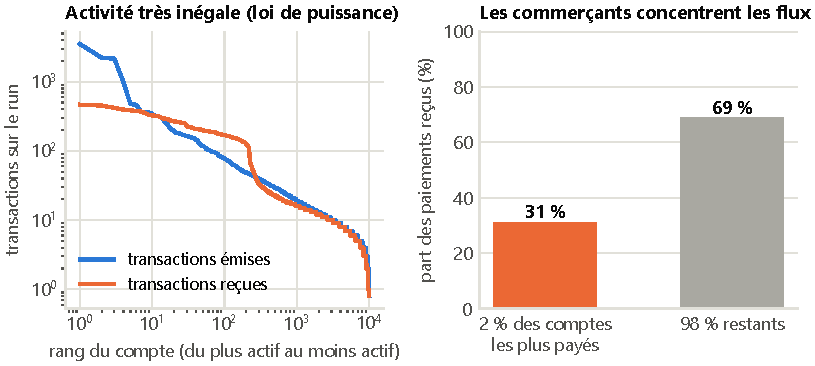
\includegraphics[width=\linewidth]{figures/activite_comptes.pdf}
\caption[Activité des comptes pendant le run]{Activité des 10\,000 comptes pendant le run d'évaluation :
quelques comptes concentrent l'essentiel des transactions (gauche, échelles logarithmiques) et
les 2\,\% de comptes les plus payés reçoivent près d'un tiers des paiements (droite).}
\label{fig:activite}
\end{figure}

Les montants dépendent du type d'opération : chaque type a un montant
médian propre et une dispersion log-normale (figure~\ref{fig:montants}). Le
seuil de 20\,000~MAD, au-dessus duquel le chemin lent construit son « graphe
des gros flux », ne retient qu'une petite minorité du trafic légitime.

\begin{figure}[htp]
\centering
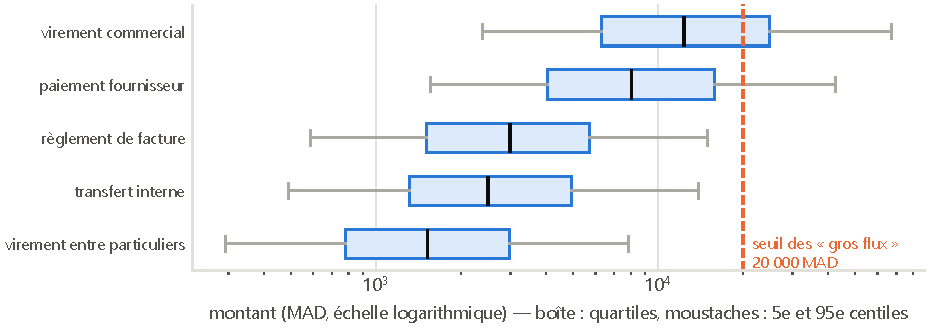
\includegraphics[width=\linewidth]{figures/montants_types.pdf}
\caption[Montants par type d'opération]{Montants par type d'opération (échantillon de 40\,000
transactions du run). Poids dans le trafic : particuliers 35\,\%, fournisseurs 20\,\%, factures 20\,\%,
commerciaux 15\,\%, internes 10\,\%.}
\label{fig:montants}
\end{figure}

\section{Les fraudes injectées}
Le producteur injecte à intervalle régulier l'une des cinq typologies du
chapitre~\ref{ch:etatart}, en choisissant des comptes « écrans » parmi le tiers
le moins actif de la population (tableau~\ref{tab:scenarios}). Les virements
d'une fraude sont étalés dans le temps et mêlés au trafic normal, comme dans
la réalité (figure~\ref{fig:scenarios}). Pour chaque fraude, le producteur
publie dans \fichier{ground-truth} son type, ses comptes, les identifiants de
ses transactions et son heure d'injection : c'est la \motcle{vérité terrain}
qui permet de calculer rappel et précision au chapitre~\ref{ch:resultats}.

\begin{table}[htp]
\centering\small
\begin{tabular}{@{}l>{\raggedright\arraybackslash}p{3.0cm}>{\raggedright\arraybackslash}p{3.3cm}>{\raggedright\arraybackslash}p{2.6cm}>{\raggedright\arraybackslash}p{2.5cm}@{}}
\toprule
\sffamily\bfseries Typologie & \sffamily\bfseries Comptes & \sffamily\bfseries Montants & \sffamily\bfseries Rythme & \sffamily\bfseries Signature\\
\midrule
{\color{cat1}\ico{F111}}~Carrousel & 3 sociétés & 40--250\,k MAD, $-$1 à 3\,\% par étape & 20--90~s entre virements & boucle fermée\\
{\color{cat3}\ico{F111}}~Cycle long & 4 ou 5 sociétés & idem & idem & boucle longue\\
{\color{cat5}\ico{F111}}~Compte mule & 8--14 émetteurs, 1 mule, 1 bénéficiaire & dépôts 2--9,8\,k ; retrait 90--97\,\% & dépôts toutes les 5--25~s & entonnoir puis vidage\\
{\color{cat4}\ico{F111}}~Scatter-gather & 1 source, 4--6 intermédiaires, 1 destination & 60--200\,k MAD répartis en parts égales & 15--60~s par relais & éventail puis regroupement\\
{\color{cat2}\ico{F111}}~Pivot & 1 pivot + 6 comptes & 3 carrousels de 60--150\,k & décalés de 10--40~s & 3 boucles, 1 compte commun\\
\bottomrule
\end{tabular}
\caption{Paramètres de génération des cinq typologies (\fichier{fraud/scenarios.py}).}
\label{tab:scenarios}
\end{table}

\begin{figure}[htp]
\centering
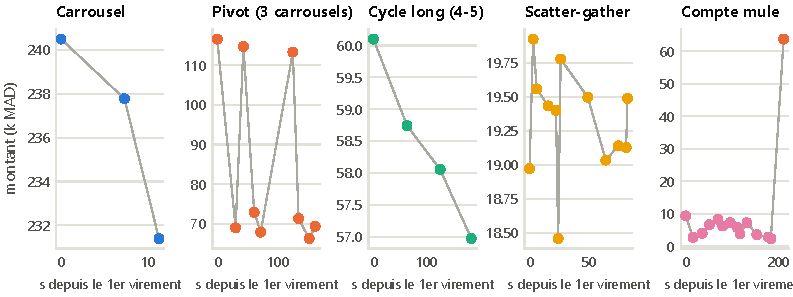
\includegraphics[width=\linewidth]{figures/scenarios_chronologie.pdf}
\caption[Chronologie de cinq fraudes réelles du run]{Chronologie d'une fraude de chaque type
injectée pendant le run : montant de chaque virement en fonction du temps écoulé depuis le premier.
On lit la commission du carrousel, les trois boucles imbriquées du pivot, la rafale de petits dépôts
de la mule suivie du retrait.}
\label{fig:scenarios}
\end{figure}

\section{Le run d'évaluation}
Toutes les figures de données de ce rapport, sauf mention contraire,
proviennent d'un même run de 42~minutes (figure~\ref{fig:trafic}) : 50
transactions par seconde, une fraude toutes les 30~secondes, après une
chauffe de 11~minutes sans fraude. Cette chauffe n'est pas un artifice : la
règle des comptes mules compare le rythme de dépôts d'un compte à son rythme
habituel, qu'il faut d'abord avoir observé.

\begin{figure}[htp]
\centering
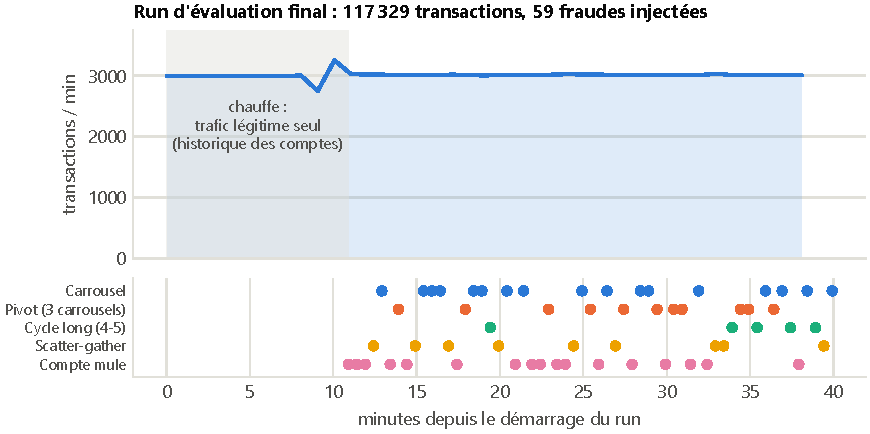
\includegraphics[width=\linewidth]{figures/trafic_run.pdf}
\caption[Trafic et fraudes injectées pendant le run d'évaluation]{Trafic et fraudes injectées pendant
le run d'évaluation. Les fraudes injectées dans les 8 dernières minutes ne comptent pas dans le
rappel, faute de temps pour être détectées : 42 fraudes sont évaluées.}
\label{fig:trafic}
\end{figure}

\section{Données imparfaites, comme en production}
Le producteur dégrade volontairement une petite partie du flux : 0,2\,\% des
messages arrivent en retard (la moitié de 30 à 100~s, l'autre moitié de 150
à 300~s, donc au-delà du watermark) et 0,05\,\% sont invalides. Le job doit
accepter les premiers, écarter les seconds, et isoler les messages invalides
dans une table de quarantaine sans jamais interrompre le flux
(figure~\ref{fig:qualite}).

\begin{figure}[htp]
\centering
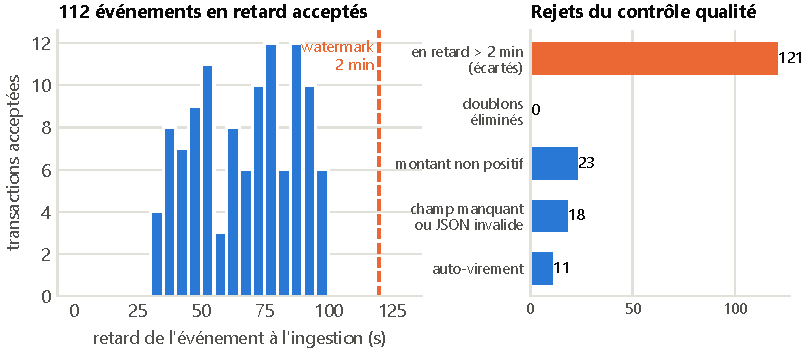
\includegraphics[width=\linewidth]{figures/qualite_donnees.pdf}
\caption[Contrôle qualité pendant le run]{Contrôle qualité pendant le run. À gauche, les événements en
retard de moins de 2~minutes sont intégrés au graphe. À droite, les 121 événements trop anciens sont
écartés par le watermark et les 52 messages invalides partent en quarantaine, avec leur motif.}
\label{fig:qualite}
\end{figure}

\aretenir{À retenir}{Le flux est réaliste (hubs, loi de puissance, retards, erreurs) et chaque fraude
injectée est connue avec précision. On peut donc \emph{mesurer} la détection plutôt que l'illustrer
sur quelques exemples choisis.}

% ============================================================
% CHAPITRE 5
% ============================================================
\chapter{Détection : du motif au score expliqué}
\label{ch:algorithmes}

\section{Chemin rapide : ne chercher que là où une boucle peut naître}
Rechercher le motif \fichier{(a)-[e1]->(b); (b)-[e2]->(c); (c)-[e3]->(a)} sur
tout le graphe glissant à chaque micro-batch revient à joindre trois fois une
table de 36\,000 arêtes avec elle-même, alors que presque rien n'a changé
depuis le lot précédent. Or une boucle \emph{nouvelle} contient forcément une
arête nouvelle. Pour une arête nouvelle $u \to v$, il suffit donc de trouver
les comptes $w$ qui reçoivent de $v$ et envoient à $u$
(figure~\ref{fig:triangle}). L'index d'adjacence en mémoire répond à cette
question par une simple intersection d'ensembles.

\begin{figure}[htp]
\centering
\begin{tikzpicture}
  \begin{scope}
    \node[compteo] (u) at (0,0) {u};
    \node[compteo] (v) at (3.0,0) {v};
    \draw[virement, color=orangeprojet, line width=1.6pt] (u) -- node[montant, above=1pt, fill=none] {arête nouvelle} (v);
    \node[compteg] (w1) at (4.5,1.2) {w\textsubscript{1}};
    \node[compteg] (w2) at (1.5,-1.75) {w\textsubscript{2}};
    \node[compteg] (w3) at (4.6,-1.3) {w\textsubscript{3}};
    \node[compteg] (w4) at (-1.5,-1.3) {w\textsubscript{4}};
    \draw[virement, color=grismoyen] (v) -- (w1);
    \draw[virement, color=bleuprojet, line width=1.3pt] (v) -- (w2);
    \draw[virement, color=grismoyen] (v) -- (w3);
    \draw[virement, color=bleuprojet, line width=1.3pt] (w2) -- (u);
    \draw[virement, color=grismoyen] (w4) -- (u);
    \node[font=\sffamily\tiny, color=encre2, align=center] at (1.5,-0.55) {triangle\\fermé};
  \end{scope}
  \begin{scope}[xshift=7.6cm, yshift=0.9cm]
    \node[anchor=north west, text width=7.2cm, font=\sffamily\scriptsize, align=left] at (0,0) {
      \textbf{Pour chaque arête nouvelle} $u \to v$ du lot :\\[3pt]
      \quad sorties de $v$ \hspace{2pt}= \{w\textsubscript{1}, w\textsubscript{2}, w\textsubscript{3}\}\\
      \quad entrées de $u$ = \{w\textsubscript{2}, w\textsubscript{4}\}\\
      \quad intersection \hspace{3pt}= \{\textbf{\color{bleuprojet}w\textsubscript{2}}\}
        $\Rightarrow$ arêtes candidates : $u{\to}v$, $v{\to}w_2$, $w_2{\to}u$\\[5pt]
      {\color{encre2}Coût proportionnel au lot et au degré des comptes concernés, pas à la taille
      du graphe. Le motif GraphFrames est ensuite exécuté sur ces seules arêtes, pour garder la
      sémantique de l'énoncé et vérifier l'ordre temporel.}};
  \end{scope}
\end{tikzpicture}
\caption{Élagage incrémental : seules les arêtes qui ferment un triangle avec une arête nouvelle
sont transmises au motif.}
\label{fig:triangle}
\end{figure}

L'effet est spectaculaire (figure~\ref{fig:elagage}) : le motif ne voit plus
qu'une centaine d'arêtes par lot au lieu de plusieurs dizaines de milliers.
C'est ce qui a fait passer le motif de 68~secondes à 0,73~seconde
(chapitre~\ref{ch:performance}).

\begin{figure}[htp]
\centering
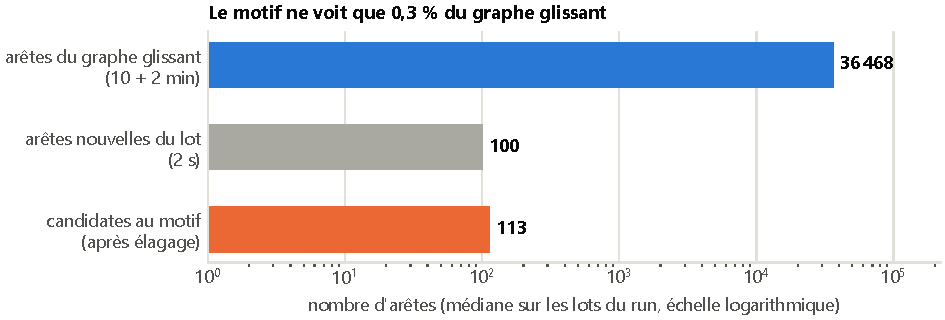
\includegraphics[width=\linewidth]{figures/elagage_candidats.pdf}
\caption[Effet de l'élagage incrémental]{Effet de l'élagage incrémental, rejoué lot par lot (lots de
2~s) sur les transactions du run : médianes sur 998 lots.}
\label{fig:elagage}
\end{figure}

\section{L'ordre temporel : une boucle doit être parcourue dans le temps}
Le motif trouve tout triangle orienté, y compris des boucles fortuites entre
commerçants où le « retour » a eu lieu \emph{avant} l'« aller ». Une boucle de
blanchiment, elle, est parcourue dans l'ordre : l'argent quitte $a$, passe
par $b$ puis $c$, et revient. La détection impose donc
$t(e_1) < t(e_2) < t(e_3)$ et une durée totale d'au plus 10~minutes. Cette
contrainte a un second effet utile : chacun des trois « tours » du même
triangle ($abc$, $bca$, $cab$) que renvoie le motif n'est retenu qu'une fois,
celui qui commence par le virement le plus ancien (figure~\ref{fig:temporel}).

\begin{figure}[htp]
\centering
\begin{tikzpicture}[
  mini/.style={circle, fill=#1, text=white, minimum size=5.5mm, inner sep=0pt, font=\sffamily\tiny\bfseries},
  t/.style={font=\sffamily\tiny, fill=white, inner sep=1pt}]
  \foreach \x/\o/\ok/\lab in {0/abc/1/{$t_1<t_2<t_3$ : retenu}, 4.1/bca/0/{$t_2<t_3$ mais $t_3 \not< t_1$ : écarté}, 8.2/cab/0/{$t_3 \not< t_1$ : écarté}} {
    \begin{scope}[xshift=\x cm]
      \ifnum\ok=1 \def\coul{orangeprojet}\else\def\coul{grismoyen}\fi
      \node[mini=\coul] (a) at (90:0.8) {a};
      \node[mini=\coul] (b) at (-30:0.8) {b};
      \node[mini=\coul] (c) at (210:0.8) {c};
      \draw[virement, color=\coul, bend left=18] (a) to node[t] {$t_1$} (b);
      \draw[virement, color=\coul, bend left=18] (b) to node[t] {$t_2$} (c);
      \draw[virement, color=\coul, bend left=18] (c) to node[t] {$t_3$} (a);
      \node[font=\sffamily\scriptsize\bfseries] at (0,1.35) {motif lu depuis {\ttfamily \o}};
      \node[font=\sffamily\tiny, color=encre2, text width=3.5cm, align=center] at (0,-1.25) {\lab};
    \end{scope}
  }
  \begin{scope}[xshift=12.3cm]
    \node[mini=grismoyen] (a) at (90:0.8) {a};
    \node[mini=grismoyen] (b) at (-30:0.8) {b};
    \node[mini=grismoyen] (c) at (210:0.8) {c};
    \draw[virement, color=grismoyen, bend left=18] (a) to node[t] {10:05} (b);
    \draw[virement, color=grismoyen, bend left=18] (b) to node[t] {10:07} (c);
    \draw[virement, color=grismoyen, bend left=18] (c) to node[t] {09:58} (a);
    \node[font=\sffamily\scriptsize\bfseries] at (0,1.35) {boucle fortuite};
    \node[font=\sffamily\tiny, color=encre2, text width=3.2cm, align=center] at (0,-1.25) {le « retour » précède l'« aller » : aucun tour n'est ordonné};
  \end{scope}
\end{tikzpicture}
\caption{Le filtre temporel retient exactement un tour de chaque vraie boucle et aucune boucle
fortuite.}
\label{fig:temporel}
\end{figure}

\section{Un score expliqué plutôt qu'une boîte noire}
Chaque boucle retenue reçoit un score de 0 à 100, somme de règles
indépendantes qui traduisent la signature d'un carrousel
(tableau~\ref{tab:score}). Chaque règle déclenchée produit une phrase, et
l'explication complète accompagne l'alerte jusque dans Kafka, Delta et le
tableau de bord. Les niveaux sont LOW ($\geq$\,20), MEDIUM ($\geq$\,40),
HIGH ($\geq$\,70) et CRITICAL ($\geq$\,90) ; seules les alertes de niveau
MEDIUM et plus sont publiées dans Kafka, toutes sont historisées.

\begin{table}[htp]
\centering\small
\begin{tabular}{@{}>{\raggedright\arraybackslash}p{5.2cm}>{\raggedright\arraybackslash}p{6.2cm}r@{}}
\toprule
\sffamily\bfseries Règle (cycles) & \sffamily\bfseries Condition & \sffamily\bfseries Points\\
\midrule
Montants quasi identiques & écart max $\leq$ 10\,\% (proches : $\leq$ 25\,\%) & 30 (15)\\
Commission régulière & perte de 0,2 à 6\,\% à \emph{chaque} étape & 15\\
Boucle rapide & bouclée en $\leq$ 5 min ($\leq$ 10 min) & 20 (10)\\
Montants élevés & $\geq$ 100\,000 MAD ($\geq$ 30\,000 ; $\geq$ 10\,000) & 15 (10 ; 5)\\
Même type d'opération & sur toute la boucle & 5\\
Compte pivot & PageRank dans le top 1\,\% (top 5\,\%) & 10 (5)\\
Cycle long & 4 sauts ou plus & 5\\
\bottomrule
\end{tabular}
\caption[Règles du score des cycles]{Règles du score des cycles (\fichier{fraud/scoring.py}). Les
mules, scatter-gather et pivots ont leurs propres grilles, construites de la même façon.}
\label{tab:score}
\end{table}

\begin{figure}[htp]
\centering
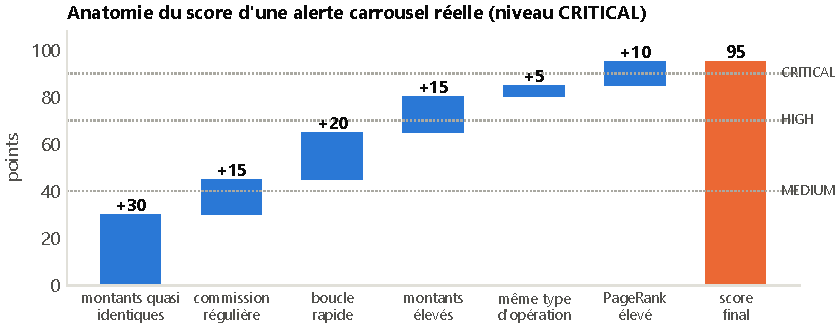
\includegraphics[width=\linewidth]{figures/score_carrousel.pdf}
\caption[Anatomie du score d'une alerte réelle]{Anatomie du score de l'alerte de la
figure~\ref{fig:carrousel}, telle qu'elle a été publiée dans Kafka.}
\label{fig:score}
\end{figure}

\begin{tcolorbox}[colback=grisclair, colframe=orangeprojet, boxrule=0pt, leftrule=3pt, arc=0pt,
  outer arc=0pt, left=8pt, right=8pt, top=5pt, bottom=5pt]
{\sffamily\bfseries\scriptsize\color{orangeprojet}ALERTE CYCLE · score 95 · CRITICAL · latence 7,0~s}\par\smallskip
\small\sffamily ACC-2801 → ACC-1853 → ACC-2052 → ACC-2801 en 2 min 27 s, 3 virements de 126\,436 MAD à
133\,500 MAD, 94,7\,\% du montant revient à l'origine. Indices : montants quasi identiques à chaque
étape (écart max 5,6\,\%) (+30) ; perte régulière de 2,7\,\% par étape (commission typique d'un
carrousel) (+15) ; boucle bouclée en 2 min 27 s (+20) ; montants élevés ($\geq$ 100\,000 MAD) (+15) ;
même type d'opération sur toute la boucle (+5) ; un compte du cycle est un pivot du réseau
(PageRank élevé) (+10).
\end{tcolorbox}

\section{Chemin lent : analyser toute la fenêtre}
Toutes les 90~secondes, le chemin lent relit dans la table bronze les
10~dernières minutes de transactions et enchaîne cinq analyses
(figure~\ref{fig:cheminlent}).

\begin{figure}[htp]
\centering
\begin{tikzpicture}[
  b/.style={draw=#1, line width=0.8pt, fill=#1!8, rounded corners=3pt, align=center,
    font=\sffamily\tiny, text width=2.25cm, minimum height=0.95cm, inner sep=2pt},
  lourd/.style={dashed, line width=1pt},
  sortie/.style={rounded corners=2pt, fill=#1, text=white, font=\sffamily\tiny\bfseries, inner sep=3pt, anchor=west},
  f/.style={-{Stealth[length=1.6mm]}, line width=0.6pt, color=encre2}]
  \node[b=bleuprojet, text width=1.9cm, minimum height=5.0cm] (win) at (0,0.55) {\textbf{fenêtre de 10 min}\\lue dans le bronze\\[3pt]$\approx$\,30\,000 arêtes};
  % gros flux
  \node[b=grismoyen] (hv) at (2.85,1.95) {\textbf{graphe des gros flux}\\$\geq$ 20\,000 MAD\\$\approx$\,2\,500 arêtes};
  % ligne A : PageRank, pivots, CC
  \node[b=bleuprojet, lourd] (pr) at (5.6,2.6) {\textbf{PageRank}\\10 itérations};
  \node[b=cat2] (pv) at (8.35,2.6) {\textbf{pivots}\\comptes dans $\geq$ 2 cycles récents};
  \node[b=cat6] (cc) at (11.1,2.6) {\textbf{Connected Components}\\comptes déjà alertés};
  % ligne B : élagage, SCC, motifs longs
  \node[b=bleuprojet, lourd] (tr) at (5.6,1.25) {\textbf{élagage} (4 tours)\\comptes sans entrée ou sans sortie retirés};
  \node[b=bleuprojet, lourd] (scc) at (8.35,1.25) {\textbf{SCC}\\sur le noyau ($\approx$\,40 arêtes)};
  \node[b=bleuprojet, lourd] (lc) at (11.1,1.25) {\textbf{motifs 4 et 5}\\dans les SCC de 4 comptes et +};
  % ligne C : mules
  \node[b=cat5] (dl) at (2.85,-0.1) {\textbf{journal des dépôts}\\40 min, en mémoire};
  \node[b=cat5] (mu) at (5.6,-0.1) {\textbf{rafale + vidage}\\rythme $\geq$ 3$\times$ l'habituel};
  % ligne D : scatter-gather
  \node[b=cat4] (sg) at (5.6,-1.35) {\textbf{motif à 2 sauts}\\\fichier{(s)->(m)->(t)}};
  % sorties
  \node[sortie=cat2] at ($(pv.south east)+(-0.75,-0.33)$) {PIVOT};
  \node[sortie=cat6] at ($(cc.east)+(0.12,0)$) {CLUSTER};
  \node[sortie=cat3] at ($(lc.east)+(0.12,0)$) {CYCLE\_LONG};
  \node[sortie=cat5] at ($(mu.east)+(0.12,0)$) {MULE};
  \node[sortie=cat4] at ($(sg.east)+(0.12,0)$) {SCATTER\_GATHER};
  % flux
  \draw[f] (win.east |- hv) -- (hv);
  \draw[f] (hv.east) -- (pr.west);
  \draw[f] (hv.east) -- (tr.west);
  \draw[f] (pr) -- (pv);
  \draw[f] (pv) -- (cc);
  \draw[f] (tr) -- (scc);
  \draw[f] (scc) -- (lc);
  \draw[f] (win.east |- dl) -- (dl);
  \draw[f] (dl) -- (mu);
  \draw[f] (win.east |- sg) -- (sg);
  \draw[f, dashed] ($(pv.north)+(0,0.55)$) node[above, font=\sffamily\tiny, color=encre2] {alertes CYCLE du chemin rapide} -- (pv.north);
  % légende
  \draw[bleuprojet, dashed, line width=1pt, rounded corners=2pt] (8.0,-0.55) rectangle (8.5,-0.25);
  \node[font=\sffamily\tiny, anchor=west, text width=4.2cm] at (8.6,-0.4) {analyse « lourde » : un passage sur deux};
\end{tikzpicture}
\caption[Les analyses du chemin lent]{Les analyses du chemin lent et les types d'alertes qu'elles
produisent. Les analyses en pointillés ne s'exécutent qu'un passage sur deux.}
\label{fig:cheminlent}
\end{figure}

\subsection*{Cycles longs : élaguer avant de chercher}
Un cycle ne peut passer que par des comptes qui reçoivent \emph{et} envoient.
Retirer itérativement les comptes sans entrée ou sans sortie réduit le graphe
des gros flux à un petit noyau, sur lequel les composantes fortement
connexes (SCC) sont calculées ; le motif à 4 ou 5 arêtes n'est cherché
qu'à l'intérieur des SCC d'au moins quatre comptes (figure~\ref{fig:grosflux}).

\begin{figure}[htp]
\centering
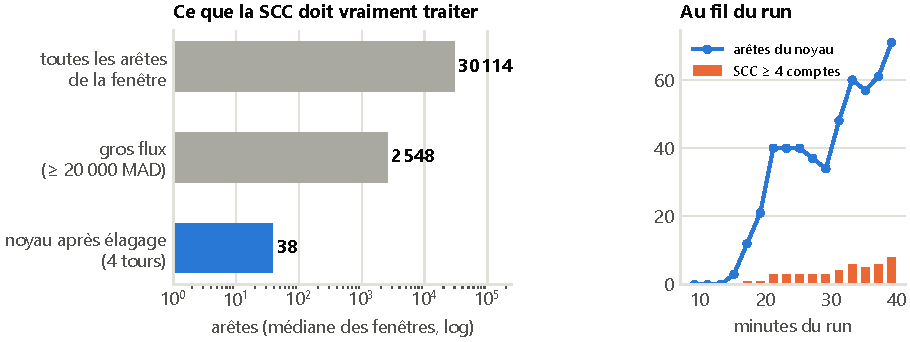
\includegraphics[width=\linewidth]{figures/elagage_gros_flux.pdf}
\caption[Réduction du graphe avant la SCC]{Réduction du graphe avant le calcul des SCC, recalculée
toutes les 2~minutes du run. Le noyau grossit au fil des fraudes injectées : il ne contient presque
que des schémas de blanchiment.}
\label{fig:grosflux}
\end{figure}

\subsection*{PageRank : un pivot n'est pas un hub}
PageRank seul désigne surtout\ldots{} les commerçants : ils reçoivent de
partout. La figure~\ref{fig:pagerank} le montre sur le dernier instantané du
run : sur les 15 comptes au plus fort PageRank, 8 sont des hubs légitimes. La
plateforme ne déclenche donc jamais d'alerte sur le PageRank seul : un compte
devient PIVOT s'il participe à au moins deux cycles suspects récents, et son
PageRank vient seulement renforcer le score.

\begin{figure}[htp]
\centering
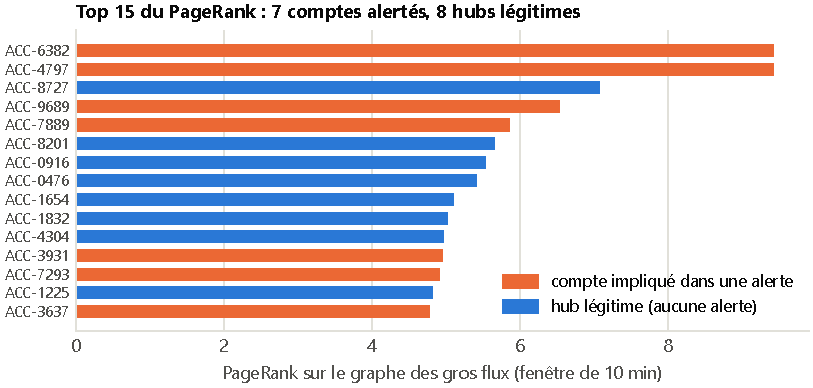
\includegraphics[width=\linewidth]{figures/pagerank_top.pdf}
\caption[PageRank : comptes alertés et hubs légitimes]{Les 15 comptes au plus fort PageRank du graphe des
gros flux à la fin du run : la moitié sont des hubs légitimes, d'où la règle combinée.}
\label{fig:pagerank}
\end{figure}

\subsection*{Comptes mules : la vélocité plutôt que le volume}
Un commerçant reçoit lui aussi beaucoup de petits paiements de nombreux
émetteurs. Ce qui distingue une mule, c'est le \emph{changement de rythme}
d'un compte habituellement calme, suivi d'un vidage. La règle finale, issue
de cinq versions mesurées contre la vérité terrain, retient un compte si,
dans les 6~minutes qui précèdent son plus gros virement sortant, il a reçu
d'au moins 6 émetteurs au moins 30\,000~MAD, à un rythme au moins trois fois
supérieur à son rythme des 20~minutes précédentes, et que ce virement unique
reprend 75 à 102\,\% des dépôts (figure~\ref{fig:mule}).

\begin{figure}[htp]
\centering
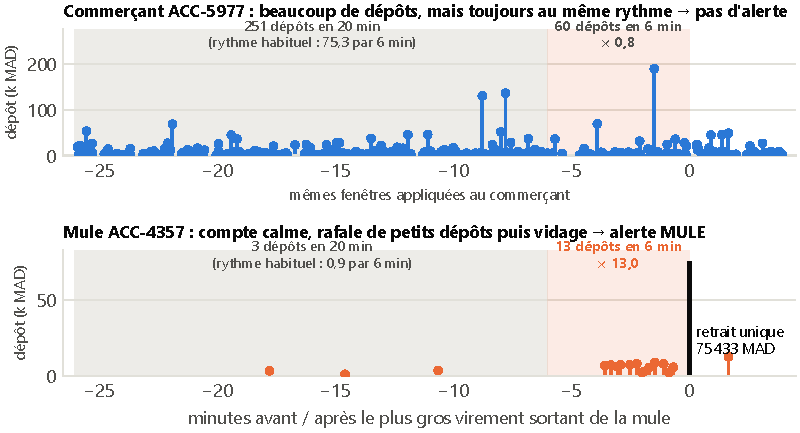
\includegraphics[width=\linewidth]{figures/mule_velocite.pdf}
\caption[Mule et commerçant face à la règle de vélocité]{La règle de vélocité appliquée à une mule
réellement détectée pendant le run et au commerçant le plus payé. Le commerçant reçoit bien plus de
dépôts, mais à son rythme habituel ($\times$\,0,8) ; la mule, elle, passe de presque rien à 13 dépôts
en 6~minutes ($\times$\,13).}
\label{fig:mule}
\end{figure}

\lecon{Ce que les versions précédentes ont appris}{Sans le critère de rythme habituel, 18 commerçants
étaient signalés comme mules. Sans la restriction aux dépôts \emph{précédant} le retrait, des dépôts
légitimes postérieurs diluaient la rafale et cachaient de vraies mules. Les deux ensemble ont fait
passer la règle de 5 mules trouvées sur 6 avec 18 fausses alertes à 12 sur 15 sans aucune fausse
alerte.}

\subsection*{Réseaux : relier les alertes}
Un pivot relie plusieurs carrousels ; plusieurs schémas peuvent partager des
comptes. Les \textbf{Connected Components} sont calculées sur le sous-graphe
des seuls comptes déjà alertés : chaque composante qui rassemble plusieurs
alertes devient une alerte CLUSTER, qui donne à l'analyste la vue d'ensemble
du réseau (figure~\ref{fig:reseau}).

\begin{figure}[htp]
\centering
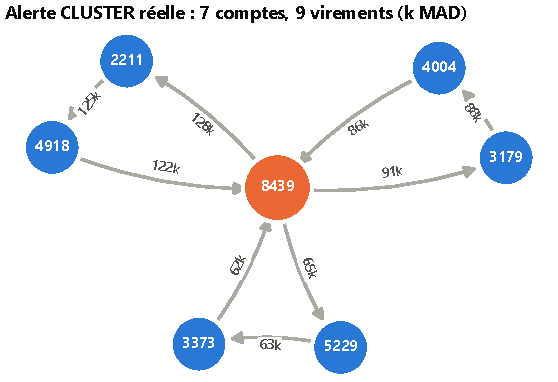
\includegraphics[width=0.78\linewidth]{figures/reseau_cluster.pdf}
\caption[Une alerte CLUSTER réelle]{Une alerte CLUSTER réelle du run : le compte ACC-8439 (en orange)
est au centre de trois carrousels imbriqués, injectés comme un seul scénario PIVOT.}
\label{fig:reseau}
\end{figure}

\section{Vue d'ensemble des alertes produites}
La figure~\ref{fig:scorestypes} place les 111 alertes de la période évaluée
selon leur type et leur score. Les fausses alertes sont presque toutes des
boucles fortuites de niveau LOW, conservées dans Delta pour l'audit mais
jamais publiées ; une seule a atteint le niveau MEDIUM.

\begin{figure}[htp]
\centering
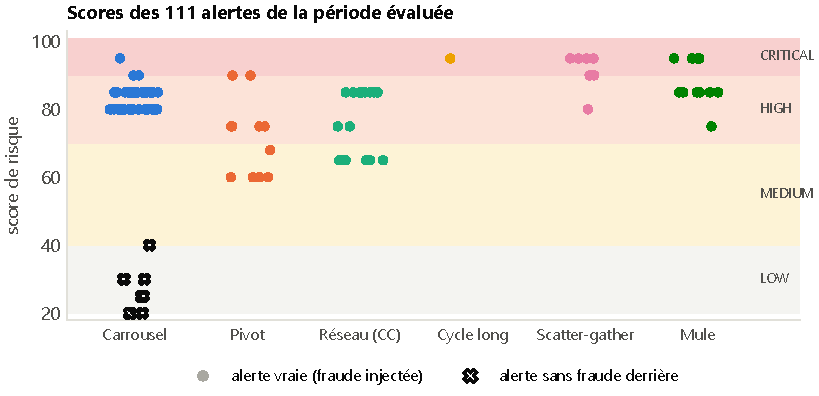
\includegraphics[width=\linewidth]{figures/scores_par_type.pdf}
\caption[Scores des alertes par type]{Score de chaque alerte de la période évaluée, par type, confronté à la
vérité terrain. Les croix sont les alertes qui ne correspondent à aucune fraude injectée.}
\label{fig:scorestypes}
\end{figure}

% ============================================================
% CHAPITRE 6
% ============================================================
\chapter{Le lakehouse Delta : historiser et auditer}
\label{ch:lakehouse}

\section{Une architecture médaillon en sept tables}
L'énoncé demande l'historisation complète des sous-graphes d'anomalies, sous
Delta Lake, partitionnée par \fichier{risk\_level} et par jour. Le lakehouse
suit l'organisation « médaillon » (figure~\ref{fig:medaillon}) : le
\motcle{bronze} garde les transactions telles qu'elles ont été acceptées, le
\motcle{silver} des données consolidées pour l'analyse, le \motcle{gold} les
alertes et leurs sous-graphes, c'est-à-dire la piste d'audit. Les sept
définitions de tables vivent dans un seul fichier,
\fichier{fraud\_graph\_delta\_schema.py}, qui sait aussi imprimer le DDL
complet (annexe~\ref{ann:ddl}).

\begin{figure}[htp]
\centering
\begin{tikzpicture}[
  couche/.style={rounded corners=4pt, draw=#1, line width=1pt, fill=#1!7, minimum width=4.75cm,
    minimum height=4.6cm},
  titre/.style={font=\sffamily\small\bfseries, color=#1},
  t/.style={draw=#1, fill=white, rounded corners=2pt, font=\ttfamily\tiny, text width=4.15cm, inner sep=3pt,
    align=left},
  prop/.style={font=\sffamily\tiny, color=encre2, text width=4.3cm, align=left}]
  \foreach \x/\c/\nom/\role in {0/bleuprojet/Bronze/{brut validé}, 5.2/cat3/Silver/{consolidé}, 10.4/orangeprojet/Gold/{métier, audit}} {
    \node[couche=\c] at (\x,0) {};
    \node[titre=\c] at (\x,2.0) {\nom};
    \node[font=\sffamily\tiny, color=encre2] at (\x,1.65) {\role};
  }
  \node[t=bleuprojet] at (0,0.85) {\textbf{transactions}\\{\sffamily partition : dt}\\{\sffamily CHECK montant > 0, pas d'auto-virement}};
  \node[t=bleuprojet] at (0,-0.35) {\textbf{transactions\_quarantine}\\{\sffamily message brut + motif du rejet}};
  \node[t=cat3] at (5.2,0.85) {\textbf{account\_metrics}\\{\sffamily PageRank, degrés, flux, SCC, cluster par compte et par instantané}};
  \node[t=cat3] at (5.2,-0.35) {\textbf{traffic\_windows}\\{\sffamily fenêtres 10 min / 1 min, MERGE}};
  \node[t=orangeprojet] at (10.4,0.95) {\textbf{fraud\_alerts}\\{\sffamily type, score, niveau, comptes, transactions, explication}};
  \node[t=orangeprojet] at (10.4,-0.05) {\textbf{anomaly\_subgraph\_vertices}\\{\sffamily comptes et rôle (ORIGINE, MULE, PIVOT\ldots)}};
  \node[t=orangeprojet] at (10.4,-0.95) {\textbf{anomaly\_subgraph\_edges}\\{\sffamily virements du sous-graphe}};
  \node[prop] at (0,-1.75) {rétention du journal : 30 jours\\écrit par le chemin rapide, \emph{après} gold};
  \node[prop] at (5.2,-1.75) {rétention du journal : 30 jours\\écrit par le chemin lent et la requête de trafic};
  \node[prop] at (10.4,-1.85) {partitions \fichier{risk\_level / dt}\\\fichier{appendOnly} : aucune modification\\journal conservé 365 jours};
  \draw[-{Stealth[length=2.2mm]}, line width=1pt, color=grismoyen] (2.45,0) -- (2.75,0);
  \draw[-{Stealth[length=2.2mm]}, line width=1pt, color=grismoyen] (7.65,0) -- (7.95,0);
\end{tikzpicture}
\caption[Le lakehouse médaillon]{Les sept tables du lakehouse, leurs contraintes et leurs propriétés.}
\label{fig:medaillon}
\end{figure}

\begin{table}[htp]
\centering\small
\begin{tabular}{@{}>{\ttfamily}l>{\ttfamily}l>{\raggedright\arraybackslash}p{8.6cm}@{}}
\toprule
\multicolumn{1}{@{}l}{\sffamily\bfseries Colonne} & \multicolumn{1}{l}{\sffamily\bfseries Type} & \sffamily\bfseries Rôle\\
\midrule
alert\_id & STRING & empreinte déterministe du type et des clés : rejouer un lot redonne le même identifiant\\
alert\_type & STRING & CYCLE, CYCLE\_LONG, MULE, SCATTER\_GATHER, PIVOT, CLUSTER\\
risk\_score, risk\_level & INT, STRING & score 0--100 (contrainte) et niveau ; \fichier{risk\_level} est une clé de partition\\
accounts, transaction\_ids & ARRAY & les comptes et les virements du schéma\\
window\_start, window\_end & TIMESTAMP & première et dernière transaction du motif\\
detected\_at, latency\_ms & TIMESTAMP, BIGINT & heure de détection et délai depuis l'ingestion Kafka\\
explanation, features & STRING & explication en français et indicateurs du score (JSON)\\
detector, dt & STRING & \fichier{fast-path} ou \fichier{slow-path} ; jour (clé de partition)\\
\bottomrule
\end{tabular}
\caption{Schéma de la table \fichier{gold/fraud\_alerts}.}
\label{tab:schemaalertes}
\end{table}

\section{Le lakehouse après les runs}
La figure~\ref{fig:delta} montre le lakehouse « vivre » pendant le run
d'évaluation : la table bronze reçoit un commit par micro-batch (près de 500
en 40~minutes), compacté périodiquement par \fichier{OPTIMIZE} pour éviter
l'accumulation de petits fichiers ; la table des alertes se répartit entre
ses partitions de niveau de risque.

\begin{figure}[htp]
\centering
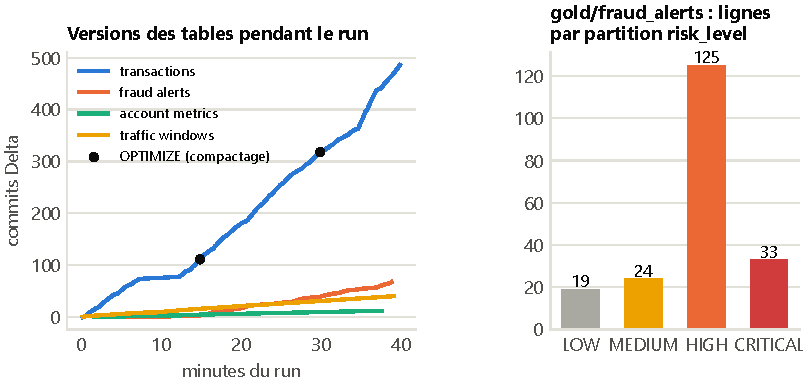
\includegraphics[width=\linewidth]{figures/delta_tables.pdf}
\caption[Les tables Delta pendant le run]{À gauche, versions des tables pendant le run d'évaluation
(journal \fichier{\_delta\_log}). À droite, contenu des partitions \fichier{risk\_level} de la table
des alertes à la fin de tous les runs (201 alertes).}
\label{fig:delta}
\end{figure}

\begin{figure}[htp]
\centering
\begin{tikzpicture}[
  dossier/.style={font=\ttfamily\scriptsize, anchor=west, inner sep=1pt},
  info/.style={font=\sffamily\tiny, color=encre2, anchor=west}]
  \node[dossier] (r) at (0,0) {\ico{F07C}~gold/fraud\_alerts/};
  \node[dossier] at (0.5,-0.45) {\ico{F15C}~\_delta\_log/ \hspace{0.3cm}{\sffamily\tiny\color{encre2} 132 versions, chaque commit = un fichier JSON}};
  \foreach \lvl/\n/\c [count=\i] in {LOW/19/grismoyen, MEDIUM/24/cat4, HIGH/125/orangeprojet, CRITICAL/33/critique} {
    \node[dossier] (l\i) at (0.5,-0.45-\i*0.45) {\color{\c}\ico{F07B}~risk\_level=\lvl/};
    \node[dossier] at (4.0,-0.45-\i*0.45) {\ico{F07B}~dt=2026-11-18/};
    \node[info] at (7.0,-0.45-\i*0.45) {\n~alertes};
  }
  \draw[grismoyen] (0.3,-0.2) -- (0.3,-2.25);
  \node[font=\sffamily\scriptsize, text width=5.4cm, align=left, anchor=west] at (8.6,-1.2) {Une requête « alertes CRITICAL
  d'aujourd'hui » ne lit qu'un dossier : c'est l'intérêt du partitionnement imposé par l'énoncé
  (\emph{partition pruning}).};
\end{tikzpicture}
\caption{Organisation physique de la table des alertes.}
\label{fig:partitions}
\end{figure}

\section{Exactly-once : une alerte une seule fois, même après une panne}
Un système d'alerte qui envoie deux fois la même alerte perd la confiance des
analystes ; un lakehouse d'audit qui contient des doublons perd sa valeur de
preuve. Spark garantit qu'un micro-batch est rejoué en entier après une panne,
mais \emph{pas} que ses effets externes n'aient pas déjà eu lieu en partie.
La plateforme combine donc trois mécanismes (figure~\ref{fig:exactlyonce}).

\begin{figure}[htp]
\centering
\begin{tikzpicture}[
  w/.style={draw=#1, line width=0.9pt, fill=#1!10, rounded corners=3pt, minimum width=2.35cm,
    minimum height=0.85cm, font=\sffamily\scriptsize, align=center},
  crash/.style={font=\sffamily\small, color=critique}]
  \node[w=grismoyen] (d) at (0,0) {détection\\{\tiny alert\_id = empreinte}};
  \node[w=orangeprojet] (k) at (3.4,0) {1 · Kafka\\{\tiny fraud-alerts}};
  \node[w=orangeprojet] (g) at (6.8,0) {2 · Delta gold\\{\tiny alertes + sous-graphes}};
  \node[w=bleuprojet] (b) at (10.2,0) {3 · Delta bronze\\{\tiny transactions}};
  \node[w=vertcode] (c) at (13.4,0) {commit du\\checkpoint};
  \foreach \a/\b in {d/k, k/g, g/b, b/c} \draw[fleche] (\a) -- (\b);
  \foreach \x/\txt in {1.7/{rejeu : même alerte, même \fichier{alert\_id}}, 5.1/{rejeu : gold ignore le doublon (\fichier{txnVersion})}, 8.5/{rejeu : bronze ignore le doublon (\fichier{txnVersion})}, 11.8/{rien à rejouer}} {
    \node[crash] at (\x,0.75) {\ico{F0E7}};
    \node[font=\sffamily\tiny, color=encre2, text width=2.9cm, align=center, anchor=north] at (\x,-0.55) {\txt};
  }
  \node[font=\sffamily\tiny\bfseries, color=critique, anchor=west] at (-1.3,0.75) {panne ici :};
\end{tikzpicture}
\caption[Ordre des écritures et reprise après panne]{Ordre des écritures d'un micro-batch et effet d'une
panne à chaque étape. Le seul doublon possible est côté Kafka, où le consommateur le reconnaît à son
\fichier{alert\_id} ; l'audit Delta reste exact.}
\label{fig:exactlyonce}
\end{figure}

\begin{itemize}
\item \textbf{Identifiants déterministes.} L'\fichier{alert\_id} est une empreinte du type et des
clés de l'alerte (transactions d'un cycle ; compte et jour d'une mule ou d'un pivot ; source,
destination et jour d'un scatter-gather). Redétecter la même fraude redonne le même identifiant.
\item \textbf{Écritures Delta idempotentes.} Chaque écriture porte le couple \fichier{txnAppId} /
\fichier{txnVersion} (identifiant de la requête, numéro du lot) : Delta ignore une écriture déjà
validée pour ce couple.
\item \textbf{Mémoire des alertes émises.} Le chemin lent, qui revoit les mêmes schémas à chaque
passage, garde l'ensemble des identifiants déjà émis, reconstruit depuis gold au démarrage.
\end{itemize}

\section{Le test de panne}
Le test rejoue la situation la plus défavorable : Spark est tué brutalement
(\fichier{docker compose kill}, équivalent d'un \fichier{kill -9}) en pleine
ingestion, pendant que le producteur continue d'écrire dans Kafka. Il est
redémarré 48~secondes plus tard ; on vérifie ensuite l'intégrité du
lakehouse (figure~\ref{fig:panne} et tableau~\ref{tab:integrite}).

\begin{figure}[htp]
\centering
\begin{tikzpicture}[x=0.0265cm]
  \draw[grismoyen, line width=0.8pt] (0,0) -- (556,0);
  \fill[orangeclair] (240,-0.18) rectangle (288,0.18);
  \fill[grisligne] (288,-0.18) rectangle (470,0.18);
  \foreach \t/\c in {0/bleuprojet, 240/critique, 288/orangeprojet, 470/vertcode, 556/vertcode}
    \fill[\c] (\t,0) circle (1.3mm);
  \tikzset{hh/.style={font=\sffamily\tiny\bfseries, color=#1}, xx/.style={font=\sffamily\tiny, align=center}}
  \node[hh=bleuprojet, anchor=south] at (0,0.15) {21:37:20};
  \node[xx, anchor=north, text width=2.6cm] at (0,-0.2) {démarrage de Spark et du producteur};
  \node[hh=critique, anchor=south] at (240,0.15) {21:41:20};
  \node[xx, anchor=north east, text width=1.7cm, align=right] at (246,-0.2) {\textbf{kill} de Spark};
  \node[hh=orangeprojet, anchor=north] at (288,-0.15) {21:42:08};
  \node[xx, anchor=south west, text width=1.6cm, align=left] at (282,0.2) {redémarrage};
  \node[hh=vertcode, anchor=south] at (470,0.15) {21:45:10};
  \node[xx, anchor=north, text width=2.8cm] at (470,-0.2) {état reconstruit : 22\,695 arêtes, 191 alertes connues};
  \node[hh=vertcode, anchor=north] at (556,-0.15) {21:46:36};
  \node[xx, anchor=south, text width=2.0cm] at (556,0.2) {contrôle d'intégrité};
\end{tikzpicture}

\vspace{4mm}
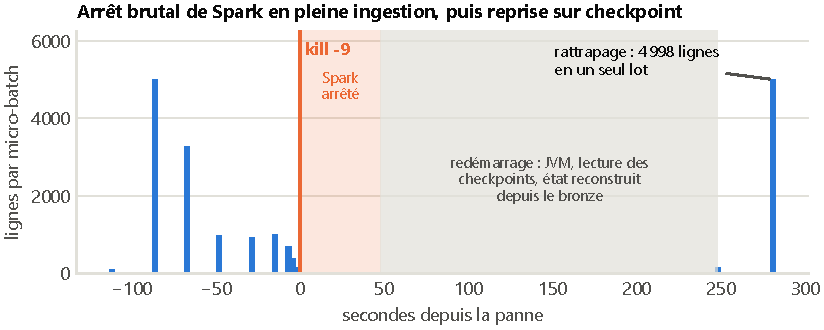
\includegraphics[width=\linewidth]{figures/panne_reprise.pdf}
\caption[Le test de panne]{Le test de panne (heures UTC). Au redémarrage, Spark relit ses checkpoints,
reconstruit son état en mémoire depuis le bronze (graphe glissant, journal des dépôts, alertes déjà
émises) puis rattrape d'un coup les messages accumulés dans Kafka.}
\label{fig:panne}
\end{figure}

\begin{table}[htp]
\centering\small
\begin{tabular}{@{}>{\raggedright\arraybackslash}p{8.5cm}rc@{}}
\toprule
\sffamily\bfseries Contrôle (\fichier{scripts/check\_integrity.py}) & \sffamily\bfseries Résultat & \\
\midrule
Transactions en double dans le bronze (même \fichier{transaction\_id}) & 0 & \oui\\
Transactions violant les contraintes métier & 0 & \oui\\
Alertes en double dans le gold (même \fichier{alert\_id}) & 0 & \oui\\
Sous-graphes sans alerte (orphelins) & 0 & \oui\\
\midrule
Transactions dans le bronze / alertes dans le gold & 201\,934 / 198 & \\
\bottomrule
\end{tabular}
\caption{Contrôle d'intégrité du lakehouse après la panne.}
\label{tab:integrite}
\end{table}

\aretenir{À retenir}{L'ordre des écritures (Kafka, puis gold, puis bronze), des identifiants
déterministes et les transactions idempotentes de Delta donnent une historisation
\emph{exactly-once} : après un arrêt brutal, aucune transaction ni aucune alerte n'est dupliquée.}

% ============================================================
% CHAPITRE 7
% ============================================================
\chapter{Le tableau de bord d'investigation}
\label{ch:dashboard}

\section{Cinq onglets, un parcours d'analyste}
Le tableau de bord (\fichier{graph\_network\_dashboard.py}, Streamlit) suit le
parcours d'un analyste : voir ce qui se passe, choisir une alerte,
l'investiguer, élargir au réseau, puis vérifier que la plateforme est saine
et que l'historique est fiable (tableau~\ref{tab:onglets}). Il lit le
lakehouse avec \fichier{delta-rs}, une implémentation de Delta Lake sans JVM :
il démarre en quelques secondes et ne consomme aucune ressource Spark.

\begin{table}[htp]
\centering\small
\begin{tabular}{@{}l>{\raggedright\arraybackslash}p{6.0cm}>{\raggedright\arraybackslash}p{5.2cm}@{}}
\toprule
\sffamily\bfseries Onglet & \sffamily\bfseries Contenu & \sffamily\bfseries Source\\
\midrule
\ico{F05B}~Vue d'ensemble & indicateurs clés, réseau suspect en direct, dernières alertes expliquées & gold, silver \fichier{traffic\_windows}\\
\ico{F0F3}~Alertes \& investigation & table filtrable, sous-graphe PyVis de l'alerte, score détaillé, fiche PDF & gold (alertes, sommets, arêtes)\\
\ico{F542}~Explorateur de réseau & voisinage à 1 ou 2 sauts d'un compte, flux entrant et sortant, PageRank & bronze, silver \fichier{account\_metrics}\\
\ico{F013}~Santé du pipeline & durée des micro-batchs par étape, latence, débit, rejets & journaux \fichier{metrics/*.jsonl}\\
\ico{F1C0}~Audit Delta Lake & partitions, historique des versions, \emph{time travel} & journal \fichier{\_delta\_log}\\
\bottomrule
\end{tabular}
\caption{Les cinq onglets du tableau de bord.}
\label{tab:onglets}
\end{table}

Deux conventions visuelles valent pour tous les graphes : la \textbf{couleur}
d'un compte ou d'une alerte est celle de son niveau de risque, toujours
accompagnée de son libellé ; la \textbf{forme} d'un sommet indique son rôle
dans le schéma (étoile : origine, losange : pivot, triangle : mule, carré :
destination). La barre latérale permet d'\textbf{injecter une fraude} de
n'importe quel type en direct, ce qui rend la démonstration reproductible
devant un jury.

\begin{figure}[htp]
\centering
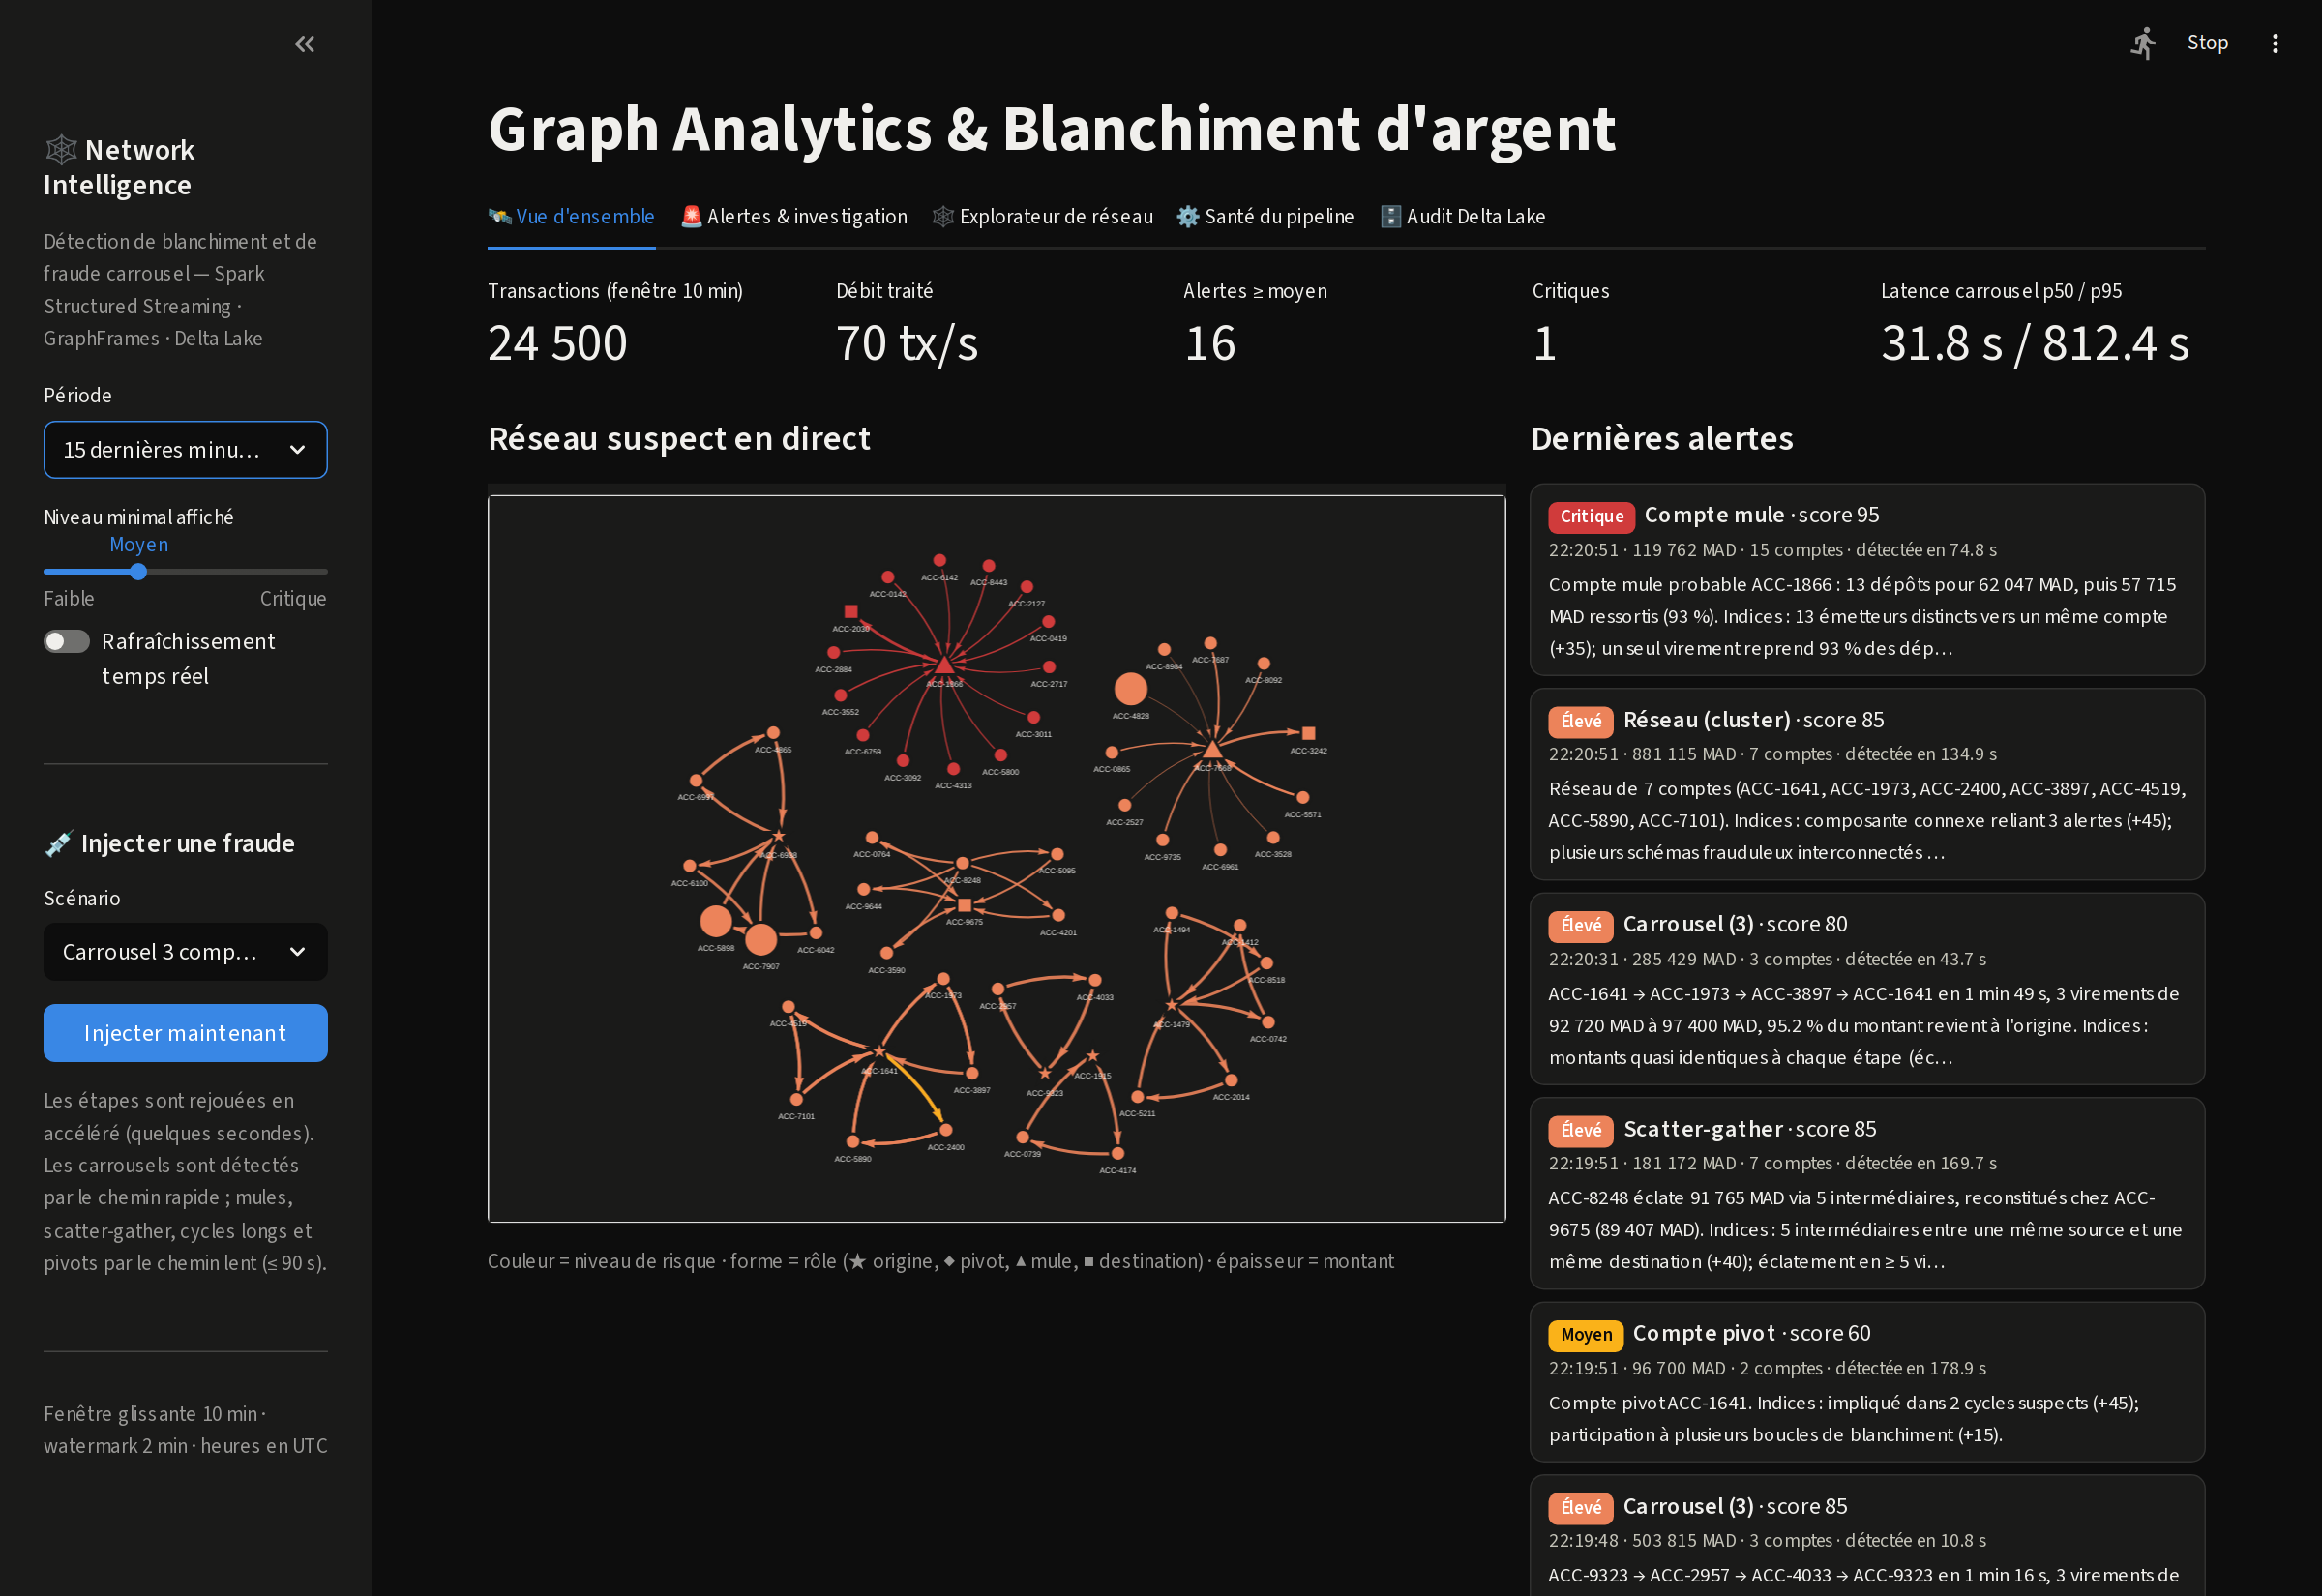
\includegraphics[width=\linewidth]{figures/captures/dashboard_vue_ensemble.png}
\caption[Vue d'ensemble du tableau de bord]{Vue d'ensemble pendant un fonctionnement réel : indicateurs
de la fenêtre courante, réseau suspect (tous les sous-graphes des alertes récentes) et dernières
alertes avec leur explication. Capture prise 7~minutes après un redémarrage : les latences affichées
incluent le rattrapage des messages accumulés pendant l'arrêt (valeurs en régime établi au
chapitre~\ref{ch:resultats}).}
\label{fig:dash1}
\end{figure}

\begin{figure}[htp]
\centering
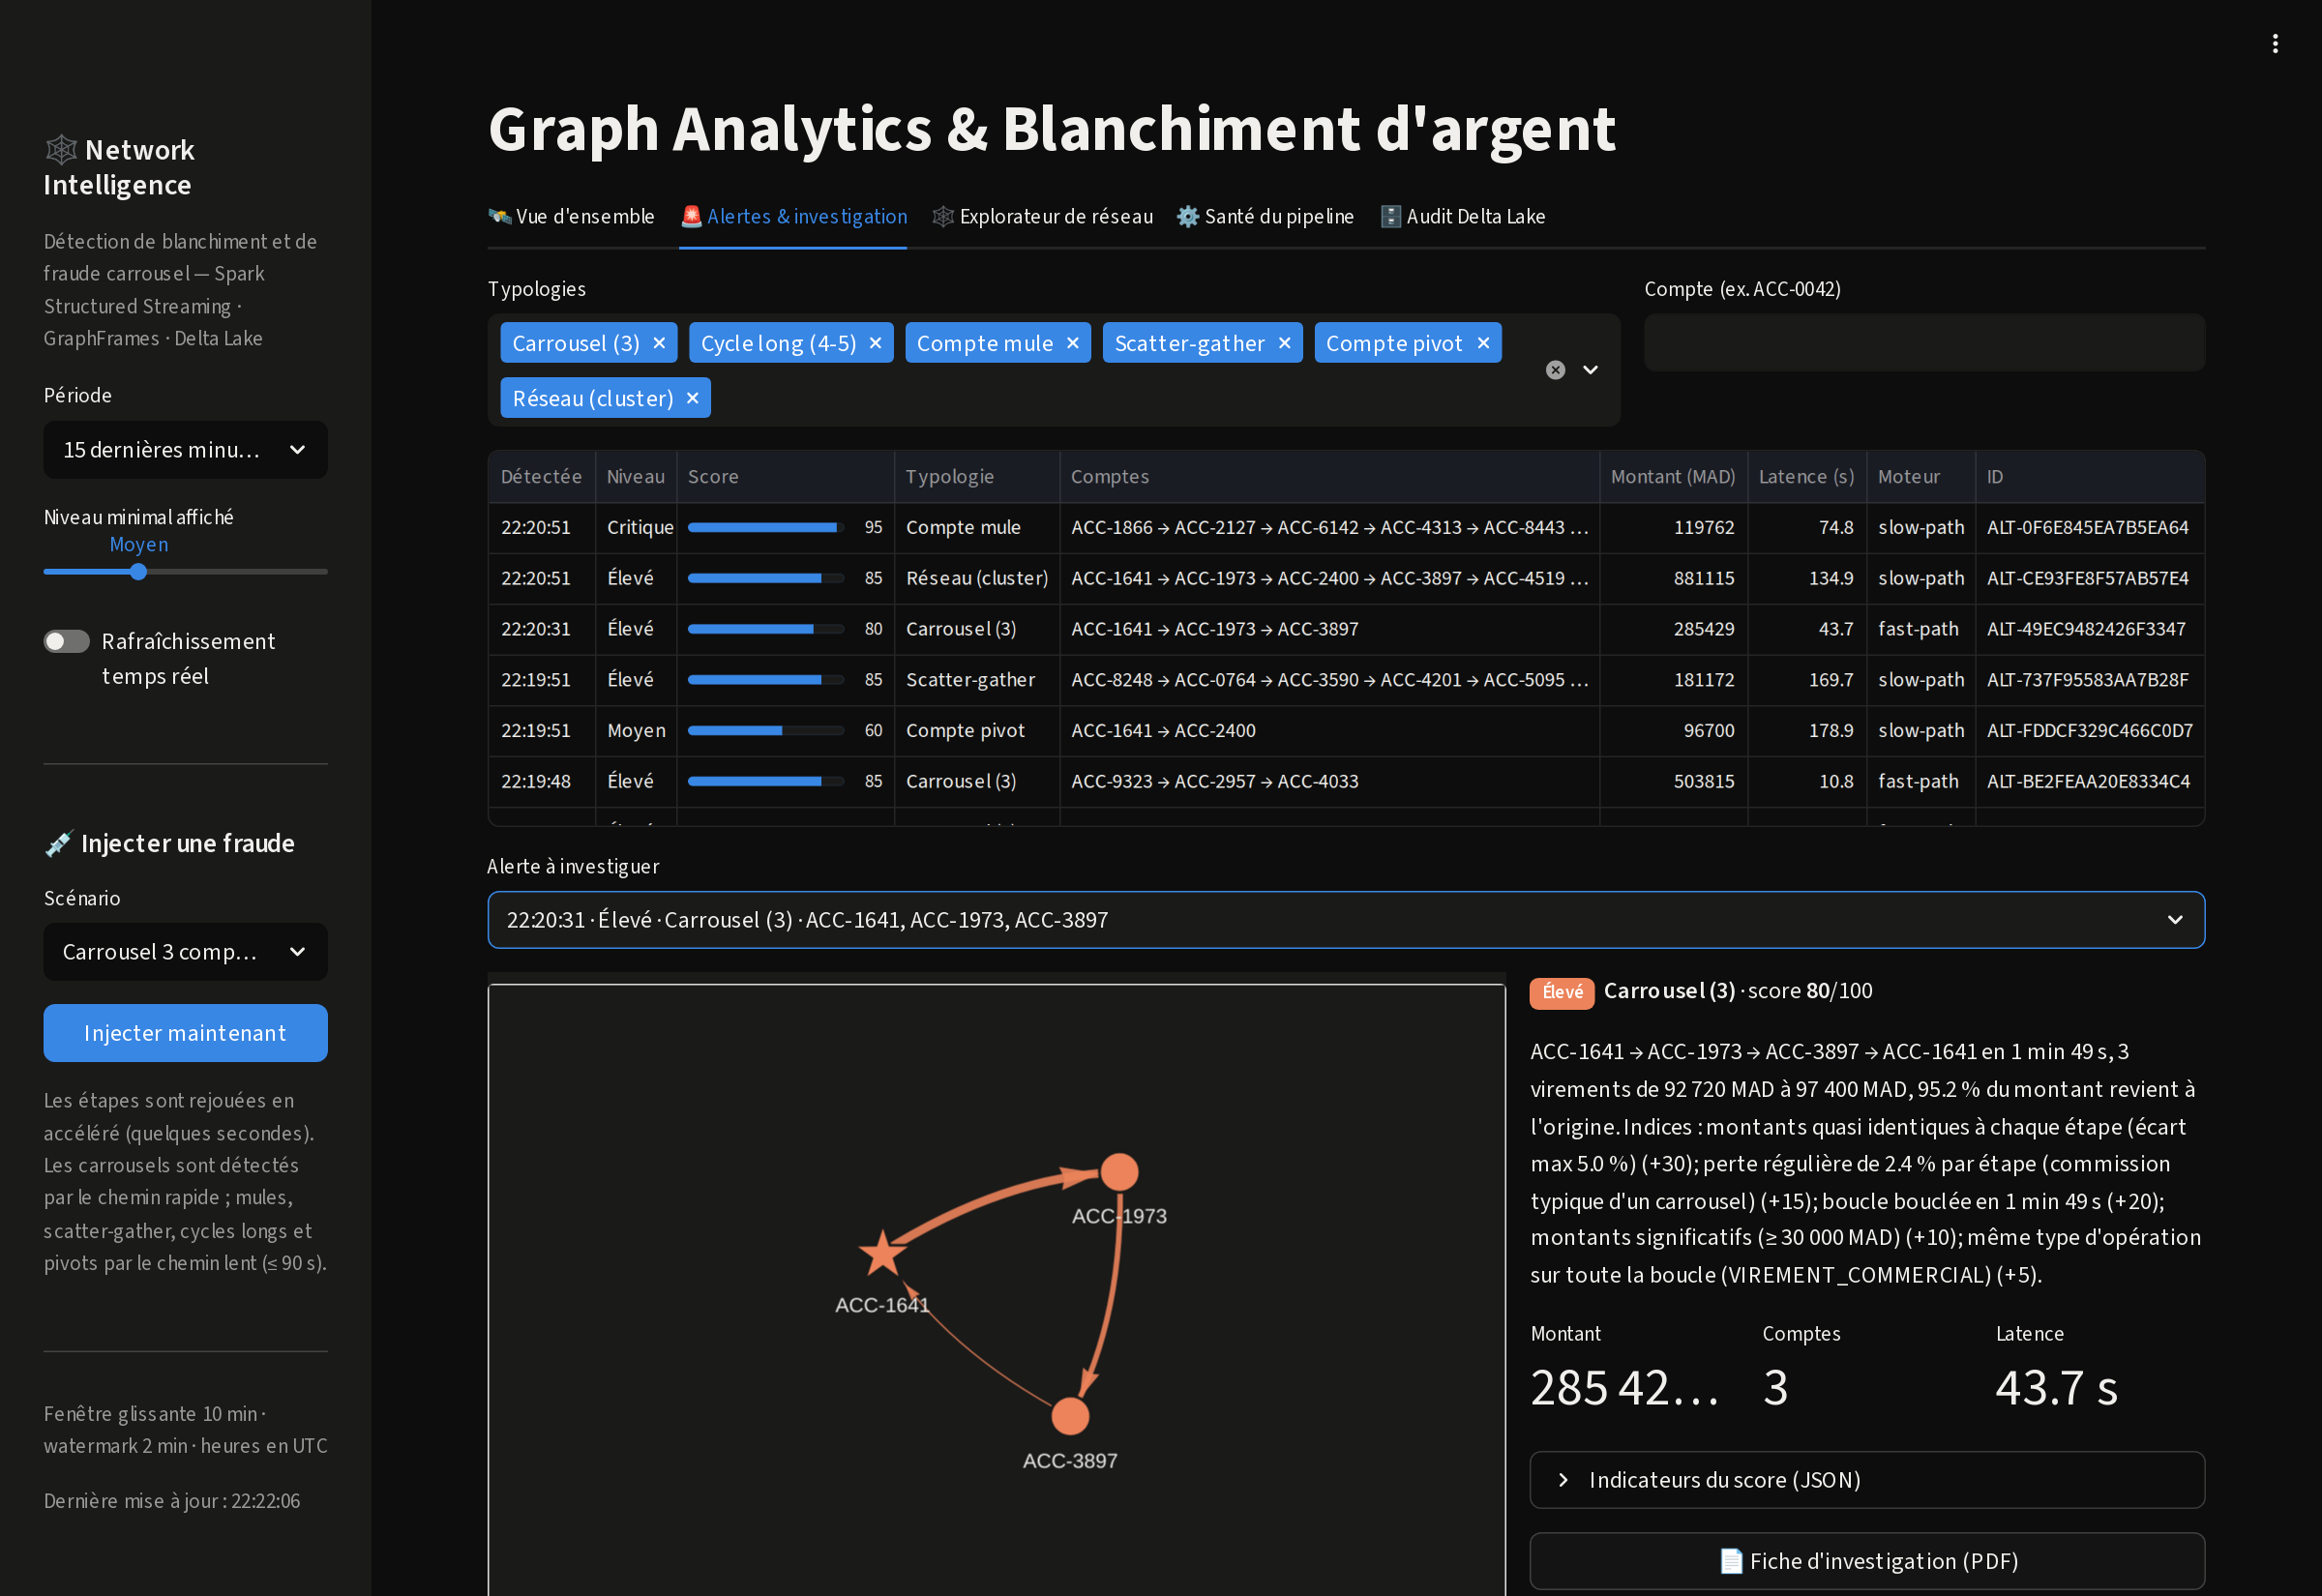
\includegraphics[width=0.495\linewidth]{figures/captures/dashboard_alertes.png}\hfill
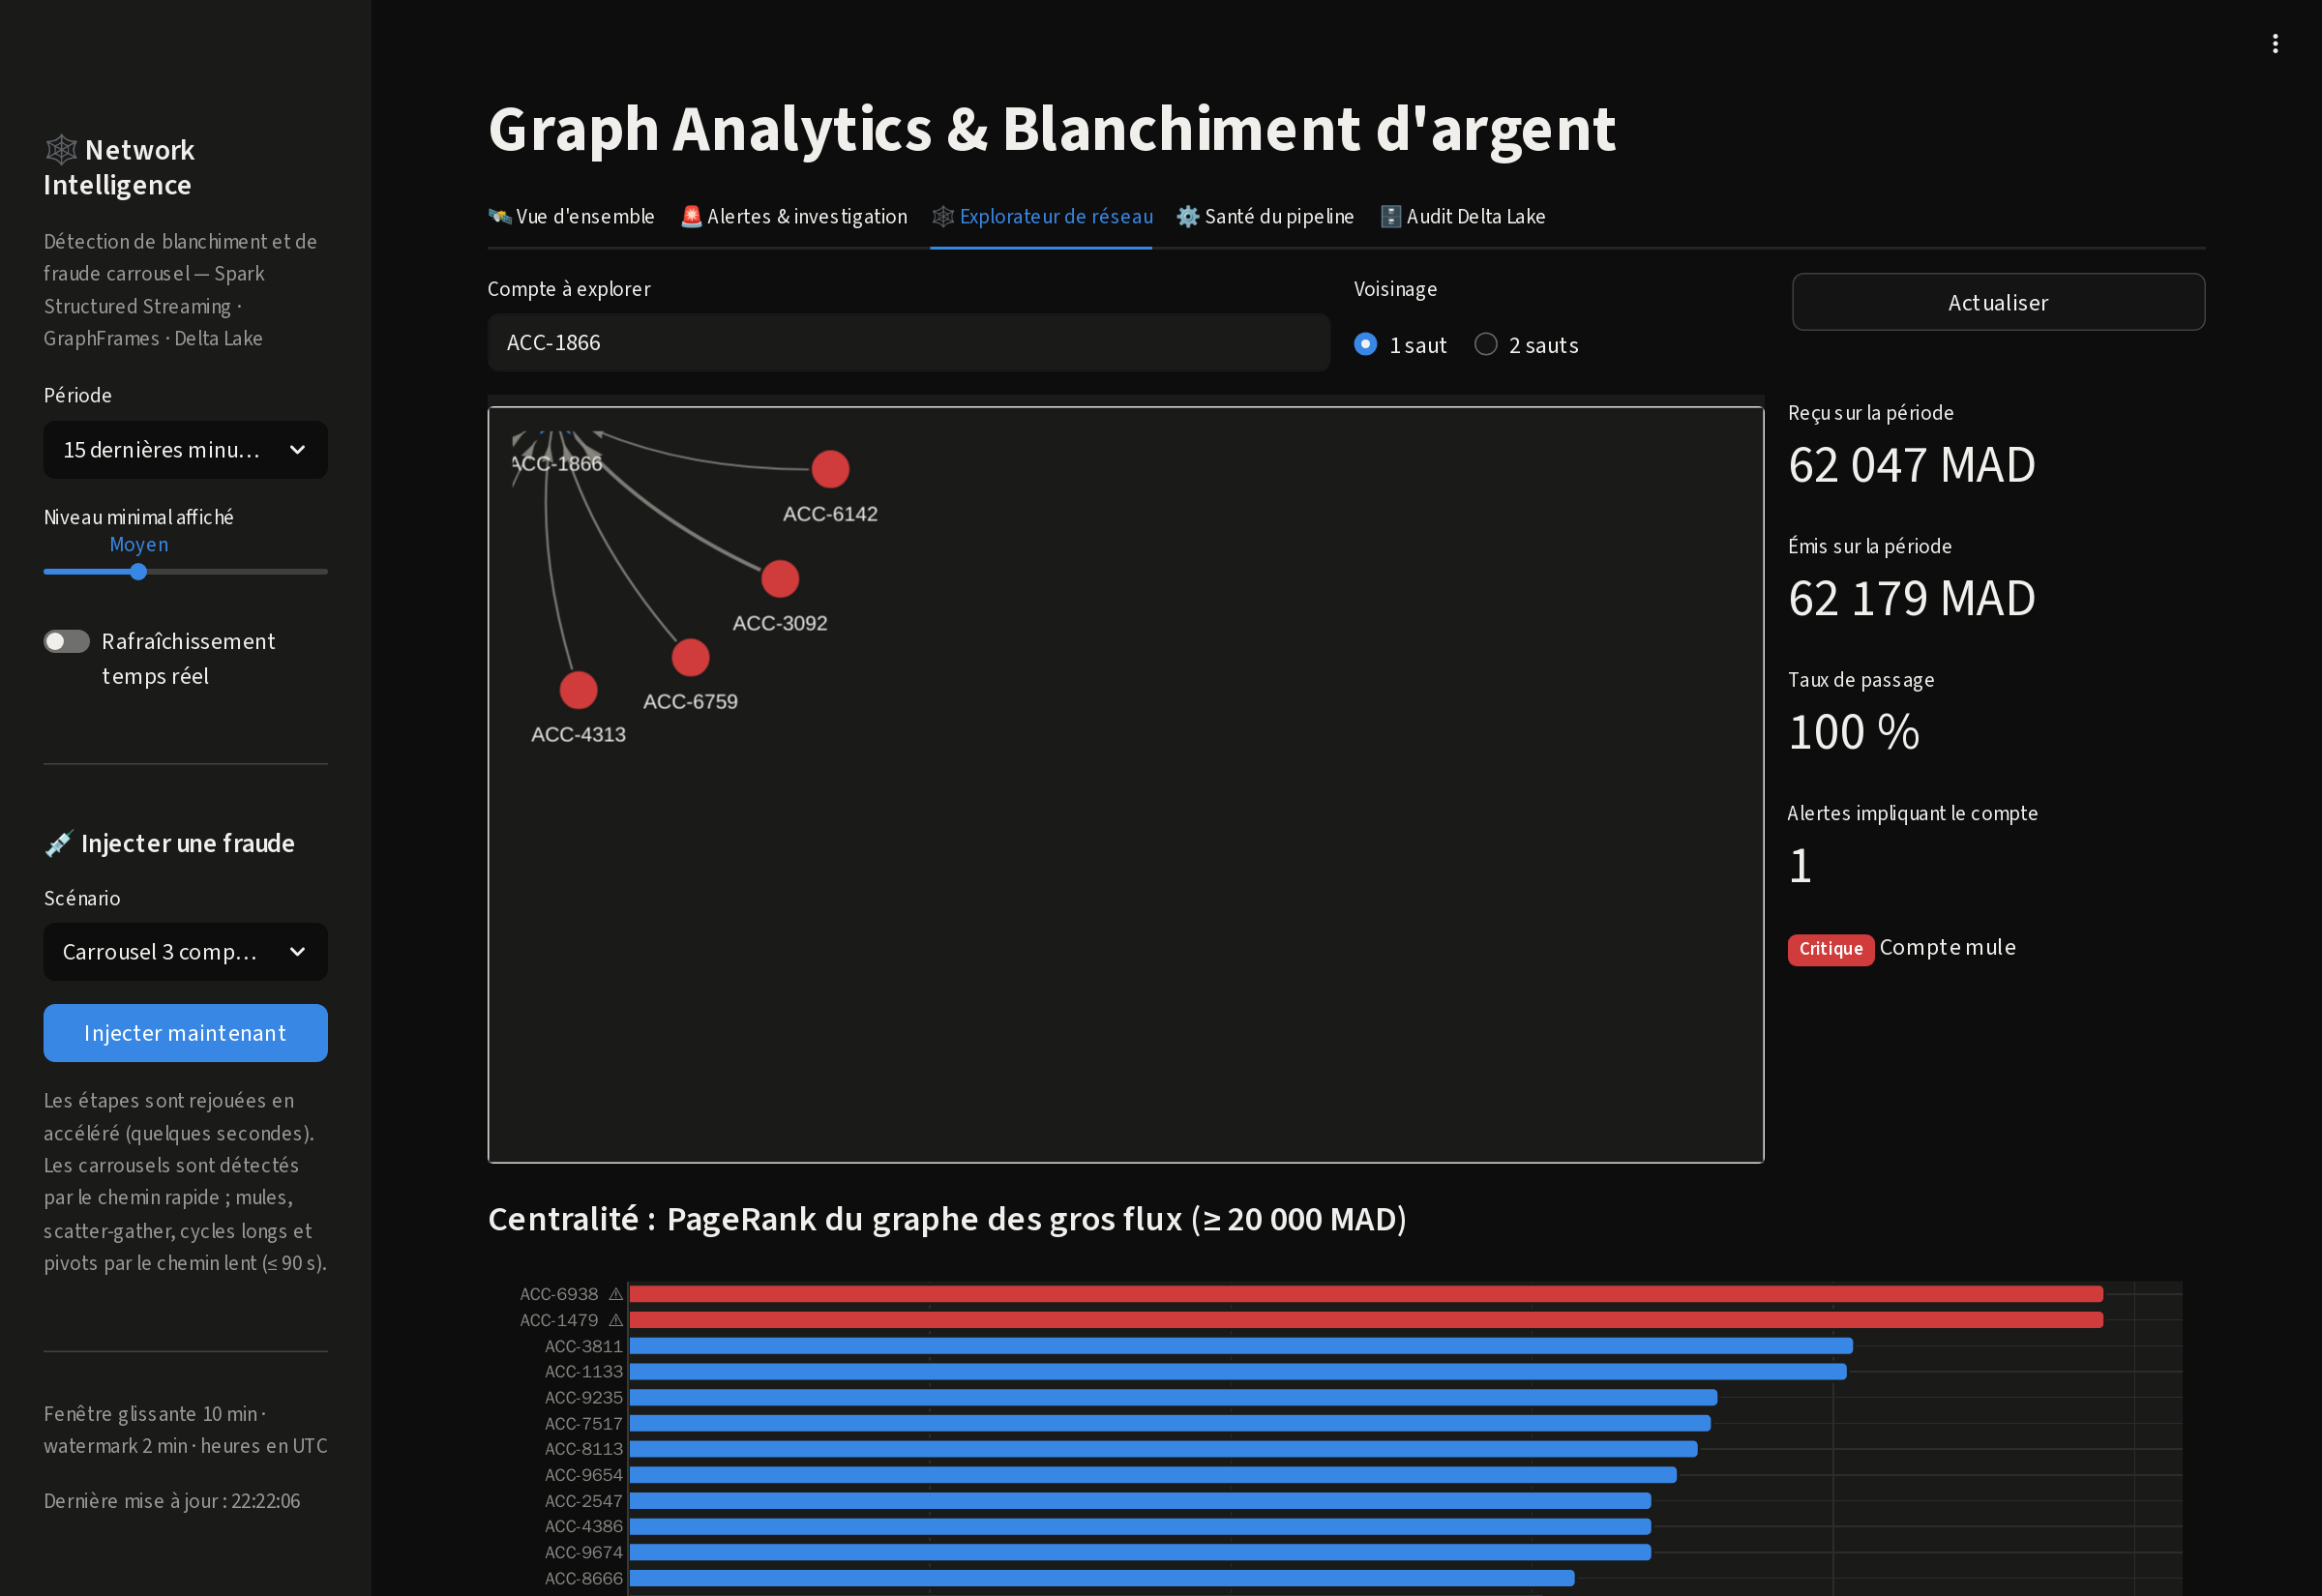
\includegraphics[width=0.495\linewidth]{figures/captures/dashboard_reseau.png}
\caption[Investigation d'une alerte et exploration du réseau]{À gauche, investigation d'une alerte :
sous-graphe interactif, score détaillé et fiche PDF téléchargeable. À droite, voisinage d'un compte
et classement PageRank du graphe des gros flux.}
\label{fig:dash2}
\end{figure}

\begin{figure}[htp]
\centering
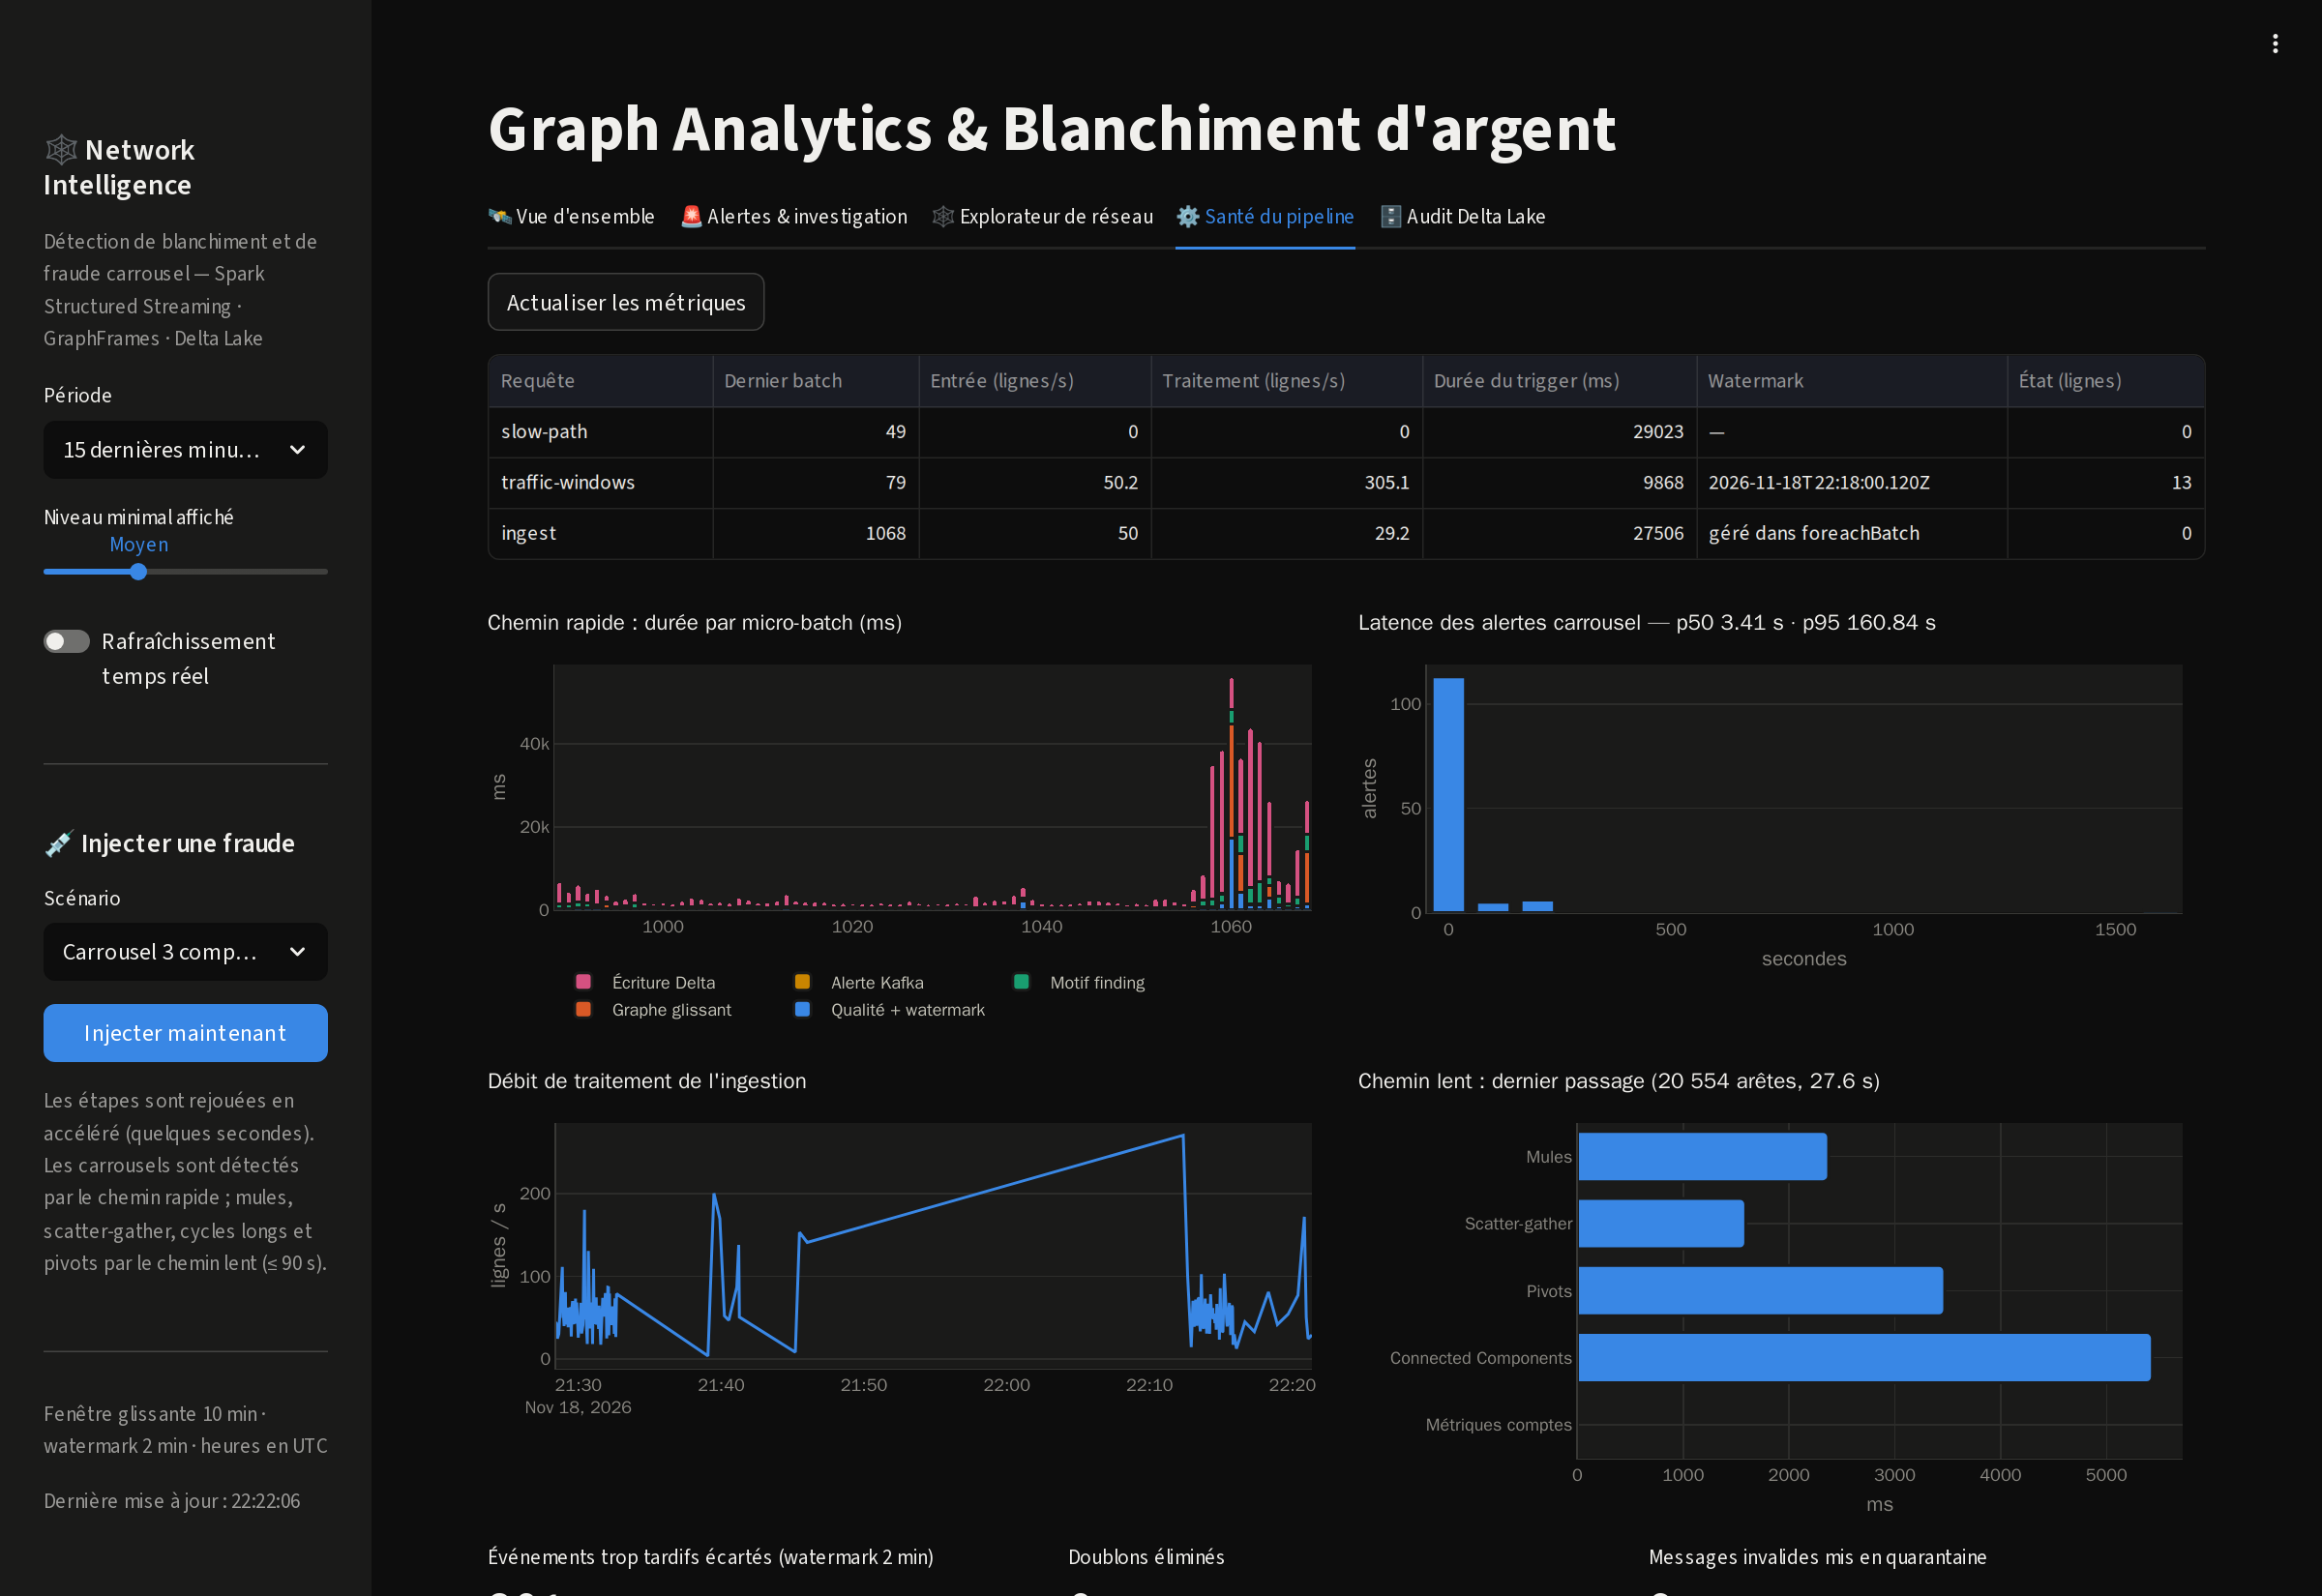
\includegraphics[width=0.495\linewidth]{figures/captures/dashboard_sante.png}\hfill
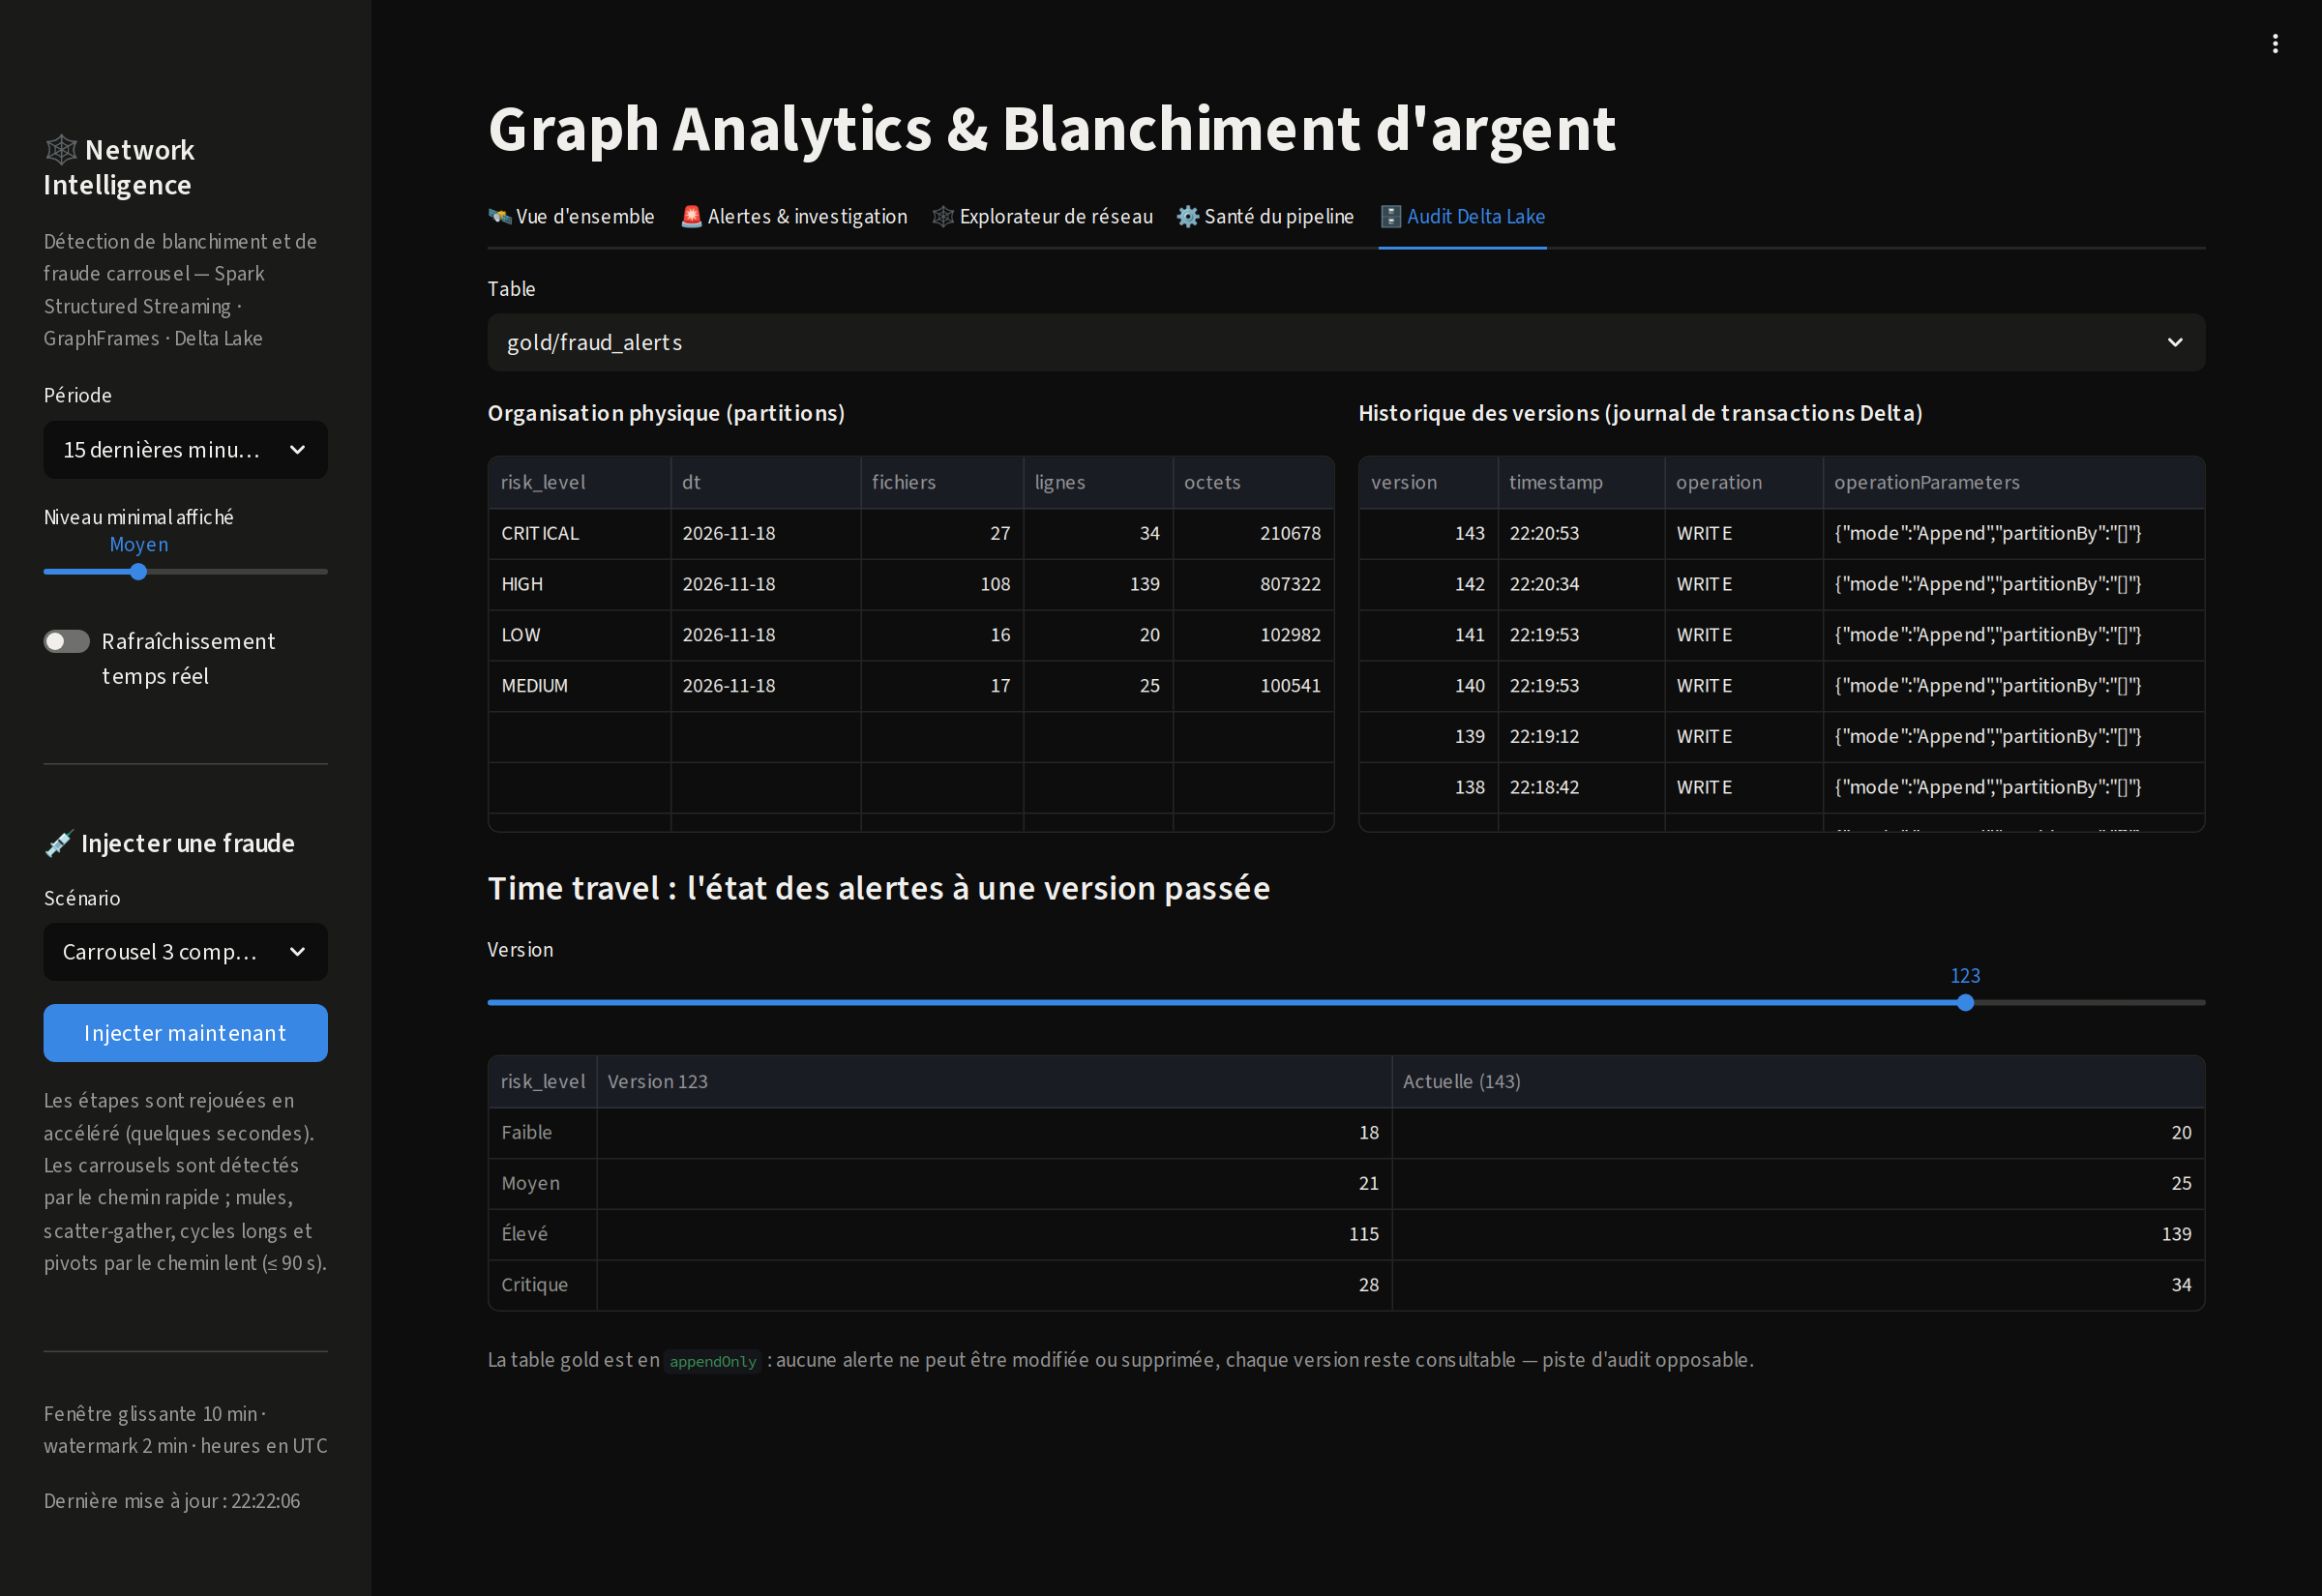
\includegraphics[width=0.495\linewidth]{figures/captures/dashboard_audit.png}
\caption[Santé du pipeline et audit Delta Lake]{À gauche, santé du pipeline : état des trois requêtes,
durée des micro-batchs décomposée par étape, latence des alertes. À droite, audit du lakehouse :
partitions, journal des versions et \emph{time travel} (état de la table des alertes à une version
passée).}
\label{fig:dash3}
\end{figure}

\section{La fiche d'investigation}
Pour chaque alerte, le tableau de bord produit une fiche PDF d'une page
(figure~\ref{fig:fiche}) : c'est le document qu'un analyste joindrait à une
déclaration de soupçon. Elle reprend l'explication en français, la liste
des comptes avec leur rôle et les virements du schéma, horodatés, et laisse
une place pour la décision de l'analyste.

\begin{figure}[htp]
\centering
\begin{minipage}[c]{0.46\linewidth}\centering
\fbox{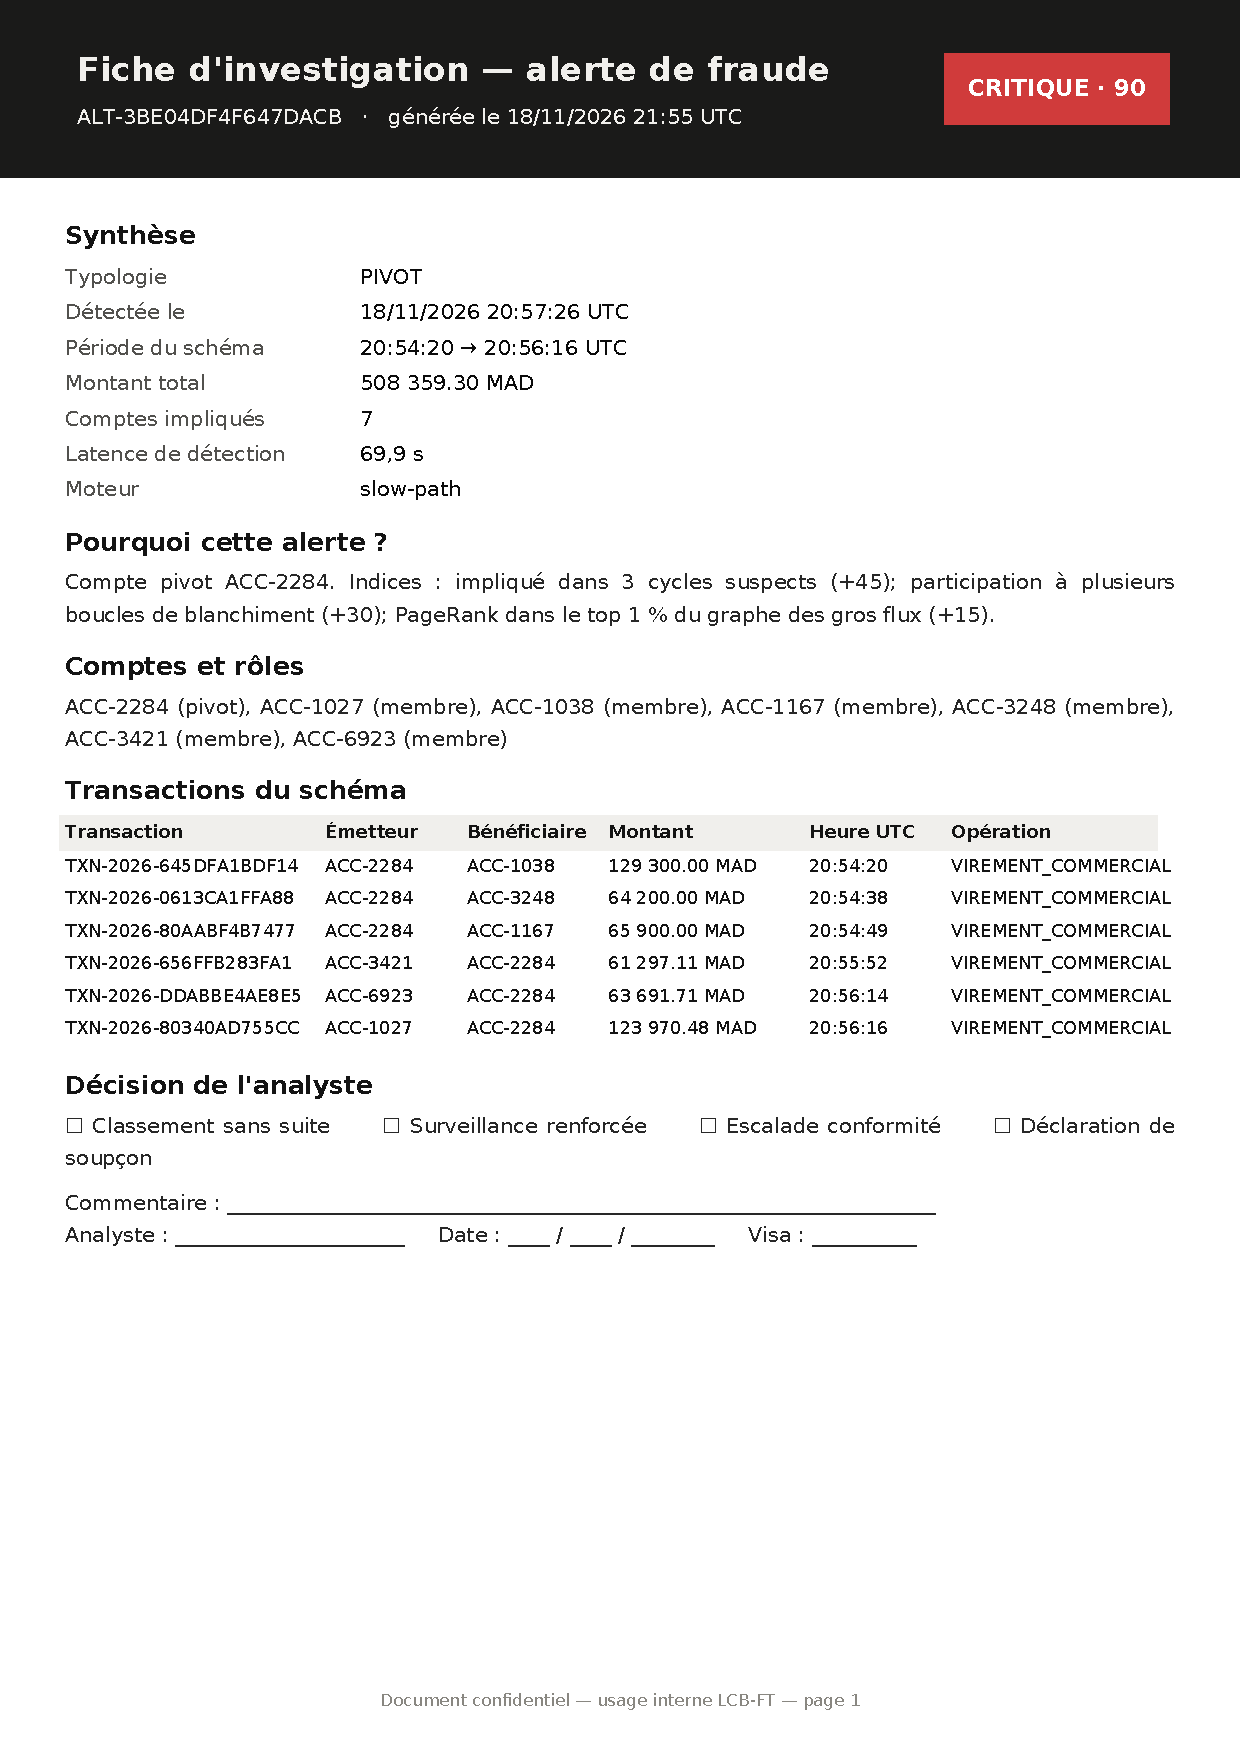
\includegraphics[width=0.92\linewidth]{figures/fiche_investigation.pdf}}
\end{minipage}\hfill
\begin{minipage}[c]{0.5\linewidth}
\begin{tikzpicture}[
  r/.style={font=\sffamily\scriptsize, text width=6.6cm, align=left, anchor=west},
  n/.style={circle, fill=bleuprojet, text=white, font=\sffamily\tiny\bfseries, minimum size=4mm, inner sep=0pt}]
  \foreach \i/\t [count=\k] in {
    1/{\textbf{En-tête} : identifiant de l'alerte, niveau et score},
    2/{\textbf{Synthèse} : typologie, période du schéma, montant, nombre de comptes, latence, moteur},
    3/{\textbf{Pourquoi cette alerte ?} L'explication en français, règle par règle},
    4/{\textbf{Comptes et rôles} dans le schéma (pivot, origine, mule, membre\ldots)},
    5/{\textbf{Transactions du schéma} : identifiant, émetteur, bénéficiaire, montant, heure},
    6/{\textbf{Décision de l'analyste} : classement, surveillance, escalade ou déclaration de soupçon, visa}} {
    \node[n] at (0,-\k*0.85) {\i};
    \node[r] at (0.3,-\k*0.85) {\t};
  }
\end{tikzpicture}
\end{minipage}
\caption[La fiche d'investigation PDF]{La fiche d'investigation générée pour une alerte PIVOT réelle du
run : le compte ACC-2284 au centre de trois carrousels (\fichier{fraud/report\_pdf.py}).}
\label{fig:fiche}
\end{figure}

% ============================================================
% CHAPITRE 8
% ============================================================
\chapter{Performances : de 97 secondes à 3,4 secondes}
\label{ch:performance}

\section{Le point de départ}
La première version fonctionnait, mais en 97~secondes par micro-batch à
100~transactions par seconde : chaque lot mettait plus longtemps à être
traité que le temps qu'il couvrait, et le retard grandissait sans fin. Ce
chapitre retrace les six versions mesurées qui ont mené à la version finale
(figure~\ref{fig:optim} et tableau~\ref{tab:optim}). Chacune a été mesurée
dans les mêmes conditions, à partir des journaux de métriques que le job
écrit à chaque lot (\fichier{metrics/fast\_path.jsonl}).

\begin{figure}[htp]
\centering
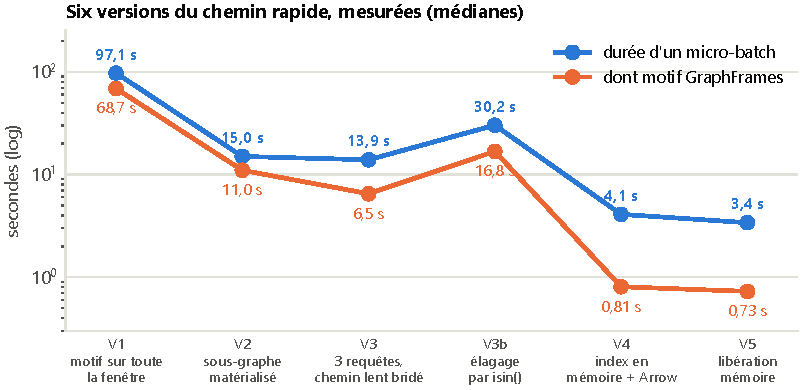
\includegraphics[width=\linewidth]{figures/optimisations.pdf}
\caption[Six versions du chemin rapide]{Durée médiane d'un micro-batch et du motif GraphFrames pour
chaque version du chemin rapide (échelle logarithmique). V1 à 100~tx/s, les suivantes à 50~tx/s.}
\label{fig:optim}
\end{figure}

\begin{table}[htp]
\centering\small
\begin{tabular}{@{}l>{\raggedright\arraybackslash}p{5.8cm}>{\raggedright\arraybackslash}p{6.4cm}@{}}
\toprule
\sffamily\bfseries & \sffamily\bfseries Changement & \sffamily\bfseries Pourquoi ça a (ou n'a pas) marché\\
\midrule
V1 & motif sur tout le graphe glissant & trois auto-jointures de dizaines de milliers d'arêtes à chaque lot\\
V2 & sous-graphe des arêtes candidates \emph{matérialisé} & non matérialisé, il était recalculé pour chaque alias du motif : 86 jobs Spark par lot, contre 6 ensuite\\
V3 & regroupement en 3 requêtes ; chemin lent sur 1--2 partitions, analyses lourdes un passage sur deux, pool FAIR & le chemin lent ne vole plus les cœurs du chemin rapide\\
V3b & élagage des candidats par \fichier{isin()} sur des listes de comptes & \textbf{régression} : chaque valeur littérale coûte un aller-retour Python--JVM\\
V4 & index d'adjacence en mémoire sur le driver ; petits DataFrames construits via Arrow puis \fichier{localCheckpoint} & l'élagage devient une intersection d'ensembles ; Spark connaît la taille des données et choisit des jointures par diffusion\\
V5 & libération explicite des checkpoints locaux ; mémoire native du JVM bornée & latence stable sur 40~minutes (section~\ref{sec:memoire})\\
\bottomrule
\end{tabular}
\caption{Ce qui a changé entre les versions, et pourquoi.}
\label{tab:optim}
\end{table}

\section{Où passe le temps aujourd'hui}
Dans la version finale, le motif GraphFrames ne prend plus que 0,73~s. Le
poste principal est désormais l'écriture dans Delta : chaque micro-batch
valide au moins une transaction Delta (bronze), et jusqu'à quatre quand il
émet une alerte (alertes, sommets et arêtes du sous-graphe) ; chacune coûte
une lecture et une écriture du journal \fichier{\_delta\_log}
(figure~\ref{fig:etapesmb}). C'est ce coût fixe, et non l'analyse de graphe,
qui sépare la plateforme d'une alerte « en sous-seconde ».

\begin{figure}[htp]
\centering
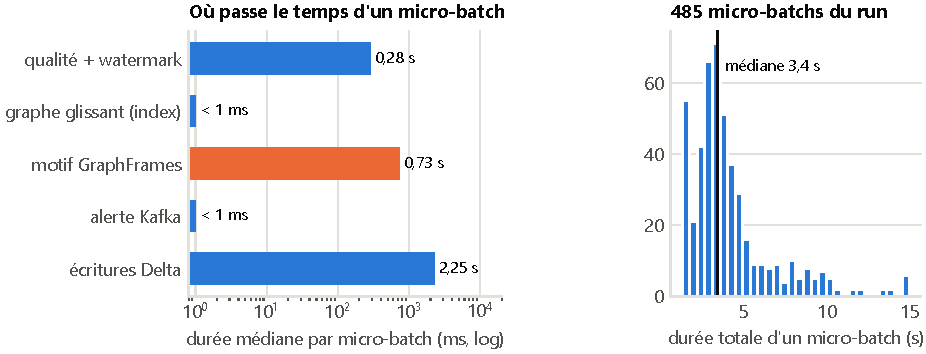
\includegraphics[width=\linewidth]{figures/etapes_microbatch.pdf}
\caption[Décomposition d'un micro-batch]{Décomposition d'un micro-batch pendant le run d'évaluation
(médianes par étape, échelle logarithmique) et distribution de la durée totale.}
\label{fig:etapesmb}
\end{figure}

\section{La mémoire : une fuite invisible}
\label{sec:memoire}
Les premiers runs longs se dégradaient au bout de 20 à 30~minutes. Deux
causes se superposaient. D'abord, \fichier{unpersist()} ne libère pas un
\fichier{localCheckpoint} : ses blocs restent en mémoire jusqu'au ramasse-miettes
périodique de Spark, et le job en accumulait plusieurs centaines (environ
2~Go en 30~minutes). Ensuite, la mémoire \emph{native} du JVM (hors tas Java)
grossissait jusqu'à la limite du conteneur. La version finale libère
explicitement chaque DataFrame matérialisé après usage, déclenche le
nettoyage de Spark toutes les 2~minutes, borne la mémoire directe du JVM
(\fichier{-XX:MaxDirectMemorySize=512m}) et limite le nombre d'arènes de
l'allocateur C (\fichier{MALLOC\_ARENA\_MAX=2}) : la mémoire se stabilise vers
3~Go (figure~\ref{fig:memoire}).

\begin{figure}[htp]
\centering
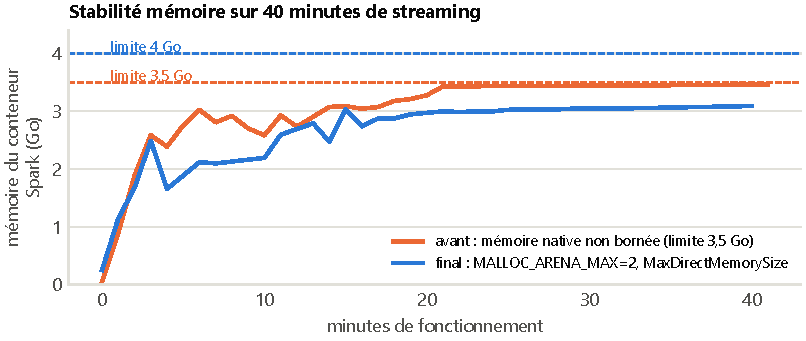
\includegraphics[width=\linewidth]{figures/memoire.pdf}
\caption[Stabilité mémoire]{Mémoire du conteneur Spark (\fichier{docker stats}) au fil de deux runs
de 40~minutes, avant et après la maîtrise de la mémoire native.}
\label{fig:memoire}
\end{figure}

\section{Le chemin lent}
Le chemin lent dispose de 90~secondes par passage. Il en utilise 32 en
médiane (figure~\ref{fig:cheminlentperf}), dont l'essentiel pour PageRank et
la SCC, exécutés un passage sur deux. Ses analyses quotidiennes --- mules,
scatter-gather, pivots --- prennent chacune une à trois secondes.

\begin{figure}[htp]
\centering
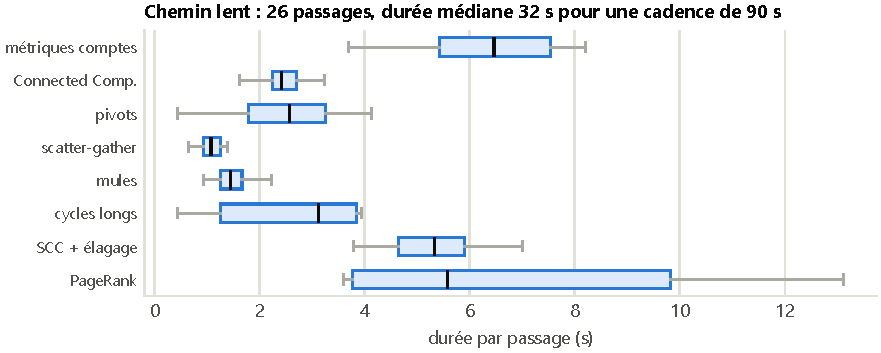
\includegraphics[width=\linewidth]{figures/chemin_lent.pdf}
\caption[Durées du chemin lent]{Durée de chaque analyse du chemin lent sur les passages du run
(boîtes : quartiles ; moustaches : étendue hors valeurs extrêmes).}
\label{fig:cheminlentperf}
\end{figure}

\section{Montée en charge}
Un benchmark injecte successivement 25, 50 et 100~transactions par seconde,
avec un carrousel toutes les 20~secondes, pendant 3~minutes par palier
(figure~\ref{fig:benchmark}). Le débit traité suit la charge et la latence de
détection des carrousels reste autour de 2~secondes : la taille des lots
augmente (50 à 177 lignes en médiane), pas leur durée, car le coût d'un lot
est dominé par ses écritures, pas par le volume.

\begin{figure}[htp]
\centering
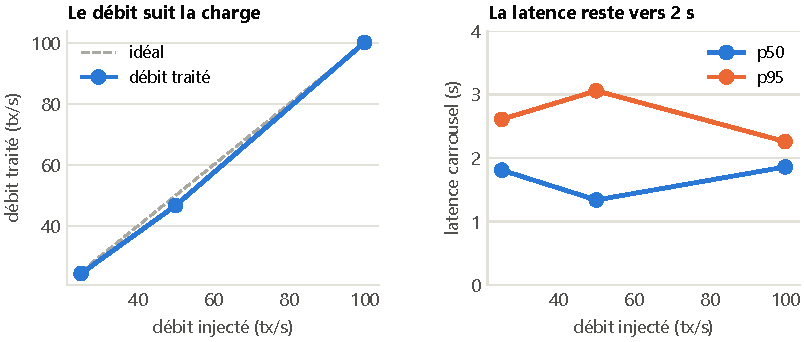
\includegraphics[width=\linewidth]{figures/benchmark.pdf}
\caption[Benchmark de montée en charge]{Benchmark de montée en charge (\fichier{scripts/benchmark.py},
producteur continu arrêté pendant la mesure, 8 carrousels injectés par palier).}
\label{fig:benchmark}
\end{figure}

\section{Leçons retenues}
Le tableau~\ref{tab:lecons} rassemble les règles qu'impose désormais le code,
chacune avec le symptôme mesuré qui l'a fait adopter. Elles sont aussi
consignées dans la documentation du dépôt (\fichier{CLAUDE.md}), pour
qu'aucune ne soit défaite sans nouvelle mesure.

\begin{table}[!htbp]
\centering\small
\begin{tabular}{@{}>{\raggedright\arraybackslash}p{6.2cm}>{\raggedright\arraybackslash}p{8.1cm}@{}}
\toprule
\sffamily\bfseries Leçon & \sffamily\bfseries Symptôme qui l'a révélée\\
\midrule
Matérialiser tout DataFrame réutilisé par un motif & 86 jobs Spark par lot au lieu de 6\\
Construire les petits DataFrames via Arrow, puis \fichier{localCheckpoint} & chaque action relançait des processus Python ($\approx$\,1~s)\\
Ne jamais passer des milliers de littéraux à \fichier{isin()} & régression de V3 à V3b (13,9~s → 30,2~s)\\
\fichier{localCheckpoint} à chaque tour d'une boucle itérative & plan d'exécution doublant à chaque tour, jusqu'à l'erreur mémoire\\
Libérer explicitement les checkpoints locaux & $\approx$\,2~Go perdus en 30~minutes, écritures Delta bloquées\\
Ne pas réactiver le state store RocksDB & arrêt brutal du JVM (« pthread lock: Invalid argument »)\\
\bottomrule
\end{tabular}
\caption{Leçons de performance, et le symptôme mesuré qui a conduit à chacune.}
\label{tab:lecons}
\end{table}

\aretenir{À retenir}{L'analyse de graphe en flux n'est rapide que si l'on ne recalcule jamais ce qui
n'a pas changé : un index incrémental en mémoire pour savoir \emph{où} chercher, GraphFrames pour
\emph{vérifier} sur un tout petit sous-graphe. Le reste est une discipline de mesure : chaque
optimisation a été validée, et une a été annulée, sur des chiffres.}

% ============================================================
% CHAPITRE 9
% ============================================================
\chapter{Résultats : qualité de détection mesurée}
\label{ch:resultats}

\section{Protocole}
La plateforme est évaluée comme une boîte noire, contre la vérité terrain
publiée par le producteur (figure~\ref{fig:protocole}). Une fraude injectée est
\emph{détectée} si une alerte de niveau MEDIUM ou plus, du type attendu,
partage au moins une transaction avec elle, ou porte sur l'un de ses comptes
clés (la mule, le pivot, la source ou la destination). Une alerte est
\emph{vraie} si elle correspond ainsi à au moins une fraude injectée. Seules
comptent pour le rappel les fraudes injectées au moins 8~minutes avant la
mesure, pour laisser au chemin lent le temps de passer.

\begin{figure}[htp]
\centering
\begin{tikzpicture}[
  b/.style={draw=#1, line width=0.9pt, fill=#1!8, rounded corners=3pt, align=center,
    font=\sffamily\scriptsize, minimum height=1.0cm, text width=2.6cm},
  f/.style={-{Stealth[length=1.9mm]}, line width=0.8pt, color=encre2}]
  \node[b=bleuprojet] (p) at (0,0) {\textbf{Producteur}\\{\tiny trafic + 1 fraude / 30 s}};
  \node[topic] (gt) at (3.4,1.0) {ground-\\truth};
  \node[topic] (tx) at (3.4,-1.0) {transactions};
  \node[b=orangeprojet] (s) at (6.8,-1.0) {\textbf{Plateforme}\\{\tiny boîte noire}};
  \node[b=orangeprojet, text width=2.2cm] (a) at (10.0,-1.0) {\textbf{alertes}\\{\tiny gold, $\geq$ MEDIUM}};
  \node[b=vertcode, text width=3.4cm, minimum height=2.9cm] (e) at (13.6,0) {\textbf{evaluate.py}\\[3pt]
    {\tiny \textbf{rappel} : fraudes détectées / fraudes injectées\\[2pt]
    \textbf{précision} : alertes vraies / alertes émises\\[2pt]
    \textbf{délai} : dernier virement de la fraude → première alerte du type attendu\\[2pt]
    \textbf{latence} : ingestion Kafka → alerte}};
  \draw[f] (p) |- (gt);
  \draw[f] (p) |- (tx);
  \draw[f] (tx) -- (s);
  \draw[f] (s) -- (a);
  \draw[f] (a) -- (a -| e.west);
  \draw[f, dashed] (gt) -- (gt -| e.west);
  \node[font=\sffamily\tiny, color=encre2] at (8.4,1.25) {jamais lue par les détecteurs};
\end{tikzpicture}
\caption{Protocole d'évaluation : la vérité terrain contourne la plateforme.}
\label{fig:protocole}
\end{figure}

\section{Rappel et précision}
Sur la période évaluée (29,5~minutes, 42~fraudes, 111~alertes), la plateforme
détecte \textbf{39 fraudes sur 42} et \textbf{101 de ses 102 alertes}
significatives correspondent à une fraude réelle (figure~\ref{fig:rp}). Toutes
les typologies sont détectées à 100\,\%, sauf les comptes mules
(12 sur 15). Deux des trois mules manquées ont été injectées dans les quatre
premières minutes après la chauffe, quand l'historique des comptes était
encore court. La seule fausse alerte est un cycle de niveau MEDIUM (score 40),
à la limite du seuil.

\aretenir{Ce que ces chiffres signifient}{Les données sont synthétiques : ces chiffres mesurent la
capacité de la plateforme à retrouver des schémas \emph{connus}, noyés dans un trafic réaliste, et non
sa performance sur de vraies fraudes, plus variées. Ils montrent en revanche trois choses solides :
la détection de forme fonctionne en flux, elle reste précise malgré les boucles fortuites du trafic
légitime, et chaque filtre de la chaîne a un effet mesuré.}

\begin{figure}[htp]
\centering
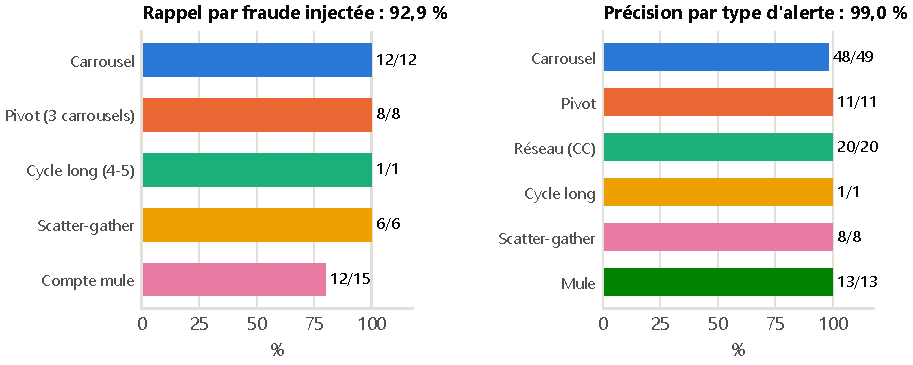
\includegraphics[width=\linewidth]{figures/rappel_precision.pdf}
\caption[Rappel et précision]{Rappel par typologie injectée (gauche) et précision par type d'alerte
(droite) sur le run d'évaluation final. Les alertes Réseau (CC) et Pivot reprennent des fraudes déjà
détectées comme carrousels : elles comptent pour la précision, pas pour le rappel.}
\label{fig:rp}
\end{figure}

\section{Délais de détection}
Le délai mesure le temps entre le \emph{dernier} virement d'une fraude --- le
moment où elle est complète --- et sa première alerte
(figure~\ref{fig:delais}). Les carrousels sont signalés en \textbf{3,9~secondes}
en médiane (8~secondes au maximum). Les autres typologies, analysées par le
chemin lent, le sont en une à deux minutes : la cadence de 90~secondes en
fixe l'ordre de grandeur. Les pivots sont signalés en 4,9~secondes en médiane
car leurs carrousels le sont dès qu'ils se ferment ; l'alerte PIVOT proprement
dite suit au passage du chemin lent.

\begin{figure}[htp]
\centering
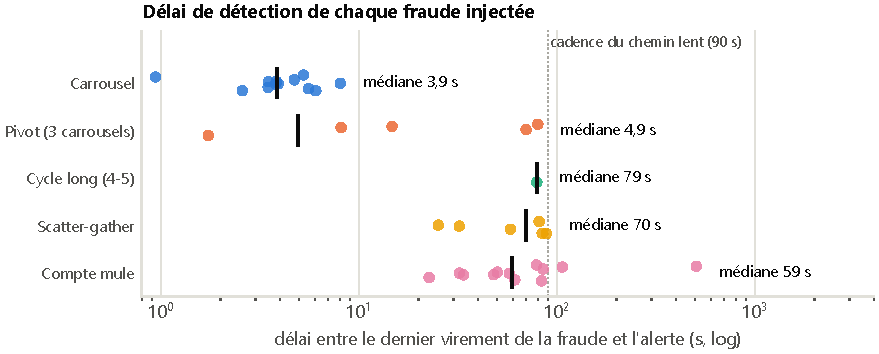
\includegraphics[width=\linewidth]{figures/delais_detection.pdf}
\caption[Délai de détection par typologie]{Délai de détection de chacune des 39 fraudes détectées
(échelle logarithmique) ; le trait noir marque la médiane.}
\label{fig:delais}
\end{figure}

\begin{figure}[htp]
\centering
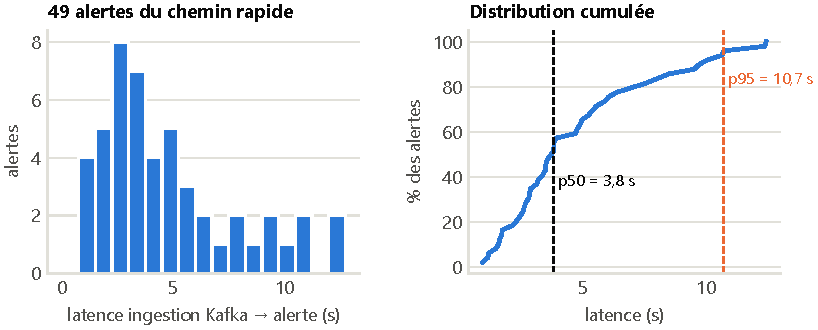
\includegraphics[width=\linewidth]{figures/latence_chemin_rapide.pdf}
\caption[Latence du chemin rapide]{Latence de bout en bout du chemin rapide, de l'ingestion de la
transaction par Kafka à la publication de l'alerte : p50 = 3,8~s, p95 = 10,7~s, p99 = 12,4~s.}
\label{fig:latence}
\end{figure}

\section{Ce qu'apporte chaque filtre : étude d'ablation}
Pour savoir si chaque étape de la détection est utile, la détection des
carrousels est rejouée hors ligne sur 90\,323 transactions d'un run
précédent, en ajoutant les filtres un à un (figure~\ref{fig:ablation}). Le
motif seul trouve 233 cycles, dont 165 boucles fortuites entre comptes très
actifs : 29\,\% de précision. L'ordre temporel élimine 142 de ces boucles
fortuites, le score 22 des 23 restantes. Aucun des 36 carrousels injectés
n'est perdu en route.

\begin{figure}[htp]
\centering
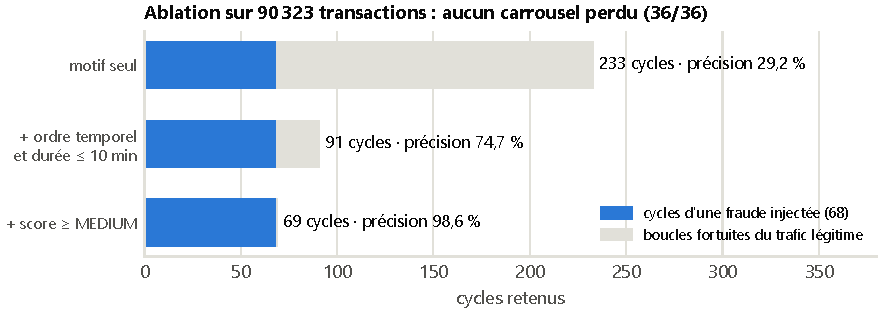
\includegraphics[width=\linewidth]{figures/ablation.pdf}
\caption[Étude d'ablation]{Étude d'ablation de la détection des carrousels
(\fichier{scripts/evaluate.py --ablation}).}
\label{fig:ablation}
\end{figure}

\section{Évolution au fil des runs}
Le run final est le cinquième run d'évaluation complet
(figure~\ref{fig:historique}). Le rappel a d'abord progressé avec la refonte
de la règle des mules (A → B), puis légèrement reculé quand la règle a été
rendue plus stricte pour éliminer les faux positifs de commerçants ; la
latence p95, elle, a révélé la fuite mémoire (C) avant d'être maîtrisée (E).

\begin{figure}[htp]
\centering
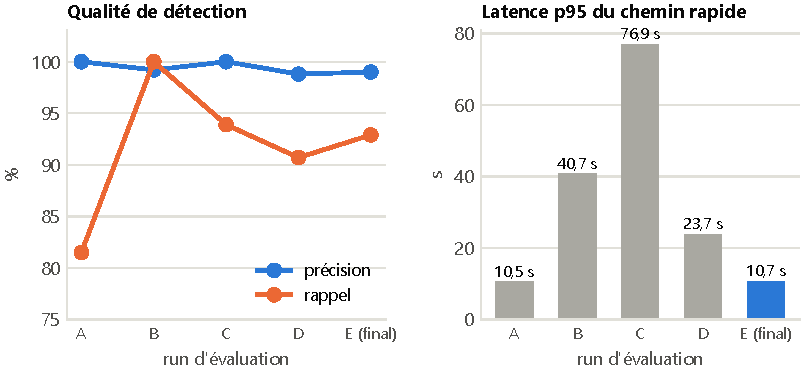
\includegraphics[width=\linewidth]{figures/historique_runs.pdf}
\caption[Cinq runs d'évaluation]{Cinq runs d'évaluation successifs. A : premier run complet ;
B : règle des mules révisée ; C : index d'adjacence et Arrow (fuite mémoire) ; D : libération
des checkpoints locaux ; E : mémoire native bornée (run final). Valeurs relevées dans
\fichier{docs/resultats.md} à chaque run.}
\label{fig:historique}
\end{figure}

\clearpage
\section{Synthèse}
Le tableau~\ref{tab:synthese} rassemble les indicateurs mesurés au fil de ce
chapitre et des précédents.

\begin{table}[h]
\centering\small
\begin{tabular}{@{}>{\raggedright\arraybackslash}p{6.2cm}>{\raggedright\arraybackslash}p{4.2cm}>{\raggedright\arraybackslash}p{3.6cm}@{}}
\toprule
\sffamily\bfseries Indicateur & \sffamily\bfseries Valeur & \sffamily\bfseries Source\\
\midrule
Précision des alertes ($\geq$ MEDIUM) & \textbf{99,0\,\%} (101 / 102) & run final\\
Rappel & \textbf{92,9\,\%} (39 / 42) & run final\\
\quad carrousels, pivots, cycles longs, scatter-gather & 100\,\% & \\
\quad comptes mules & 80\,\% (12 / 15) & \\
Délai de détection d'un carrousel & \textbf{3,9~s} médiane, 8,1~s max & run final\\
Latence du chemin rapide & 3,8~s (p50), 10,7~s (p95) & run final\\
Débit soutenu & 100~tx/s sans dérive & benchmark\\
Précision des carrousels : motif seul → final & 29\,\% → 99\,\% sans perte & ablation\\
Doublons après un arrêt brutal de Spark & \textbf{0} & test de panne\\
\bottomrule
\end{tabular}
\caption{Synthèse des résultats mesurés.}
\label{tab:synthese}
\end{table}

% ============================================================
% CHAPITRE 10
% ============================================================
\chapter{Tests et qualité logicielle}
\label{ch:qualite}

\section{Trois niveaux de vérification}
La plateforme est vérifiée à trois niveaux (figure~\ref{fig:pyramide}). Les
tests unitaires en Python pur s'exécutent en une seconde et couvrent la
logique métier ; les tests Spark démarrent une vraie session avec GraphFrames
et Delta Lake pour vérifier les motifs et le schéma ; les mesures de bout en
bout (évaluation, ablation, benchmark, test de panne) vérifient la plateforme
entière sur des données réalistes.

\begin{figure}[htp]
\centering
\begin{tikzpicture}
  \fill[vertcode!80] (-4.6,0) -- (4.6,0) -- (3.45,1.15) -- (-3.45,1.15) -- cycle;
  \fill[bleuprojet!80] (-3.4,1.25) -- (3.4,1.25) -- (2.25,2.4) -- (-2.25,2.4) -- cycle;
  \fill[orangeprojet!85] (-2.2,2.5) -- (2.2,2.5) -- (1.1,3.65) -- (-1.1,3.65) -- cycle;
  \node[font=\sffamily\scriptsize\bfseries, text=white, align=center] at (0,0.57) {19 tests unitaires (Python pur)\\[-1pt]{\tiny\mdseries scénarios, score, index glissant, vélocité, identifiants}};
  \node[font=\sffamily\scriptsize\bfseries, text=white, align=center] at (0,1.82) {10 tests Spark\\[-1pt]{\tiny\mdseries motifs, SCC, CC, mules, schéma Delta}};
  \node[font=\sffamily\tiny\bfseries, text=white, align=center] at (0,3.02) {bout en bout\\[-1pt]{\tiny\mdseries 4 mesures}};
  \foreach \y/\t in {0.57/{$\approx$\,1~s · sur l'hôte comme en CI}, 1.82/{$\approx$\,2~min · dans l'image Docker (JVM)}, 3.07/{30--45~min · sur la plateforme complète}}
    \node[font=\sffamily\scriptsize, anchor=west, color=encre2] at (4.9,\y) {\t};
\end{tikzpicture}
\caption{Les trois niveaux de vérification : 29 tests automatisés et quatre mesures de bout en bout.}
\label{fig:pyramide}
\end{figure}

\begin{table}[htp]
\centering\small
\begin{tabular}{@{}>{\raggedright\arraybackslash}p{6.9cm}>{\raggedright\arraybackslash}p{7.3cm}@{}}
\toprule
\sffamily\bfseries Test (extraits) & \sffamily\bfseries Ce qu'il garantit\\
\midrule
\fichier{test\_triangle\_temporal\_unique\_rotation} & un carrousel n'est signalé qu'une fois, pas trois\\
\fichier{test\_triangle\_out\_of\_order\_rejected\ldots} & une boucle non ordonnée dans le temps est écartée\\
\fichier{test\_incremental\_search\_only\_reports\ldots} & le chemin rapide ne redétecte pas les anciens cycles\\
\fichier{test\_long\_cycle\_found\_inside\_scc} & un cycle de 5 comptes est trouvé dans sa SCC\\
\fichier{test\_mule\_velocity\_spike\_excludes\ldots} & un commerçant régulier n'est pas une mule\\
\fichier{test\_alert\_id\_is\_deterministic\ldots} & même fraude, même identifiant (exactly-once)\\
\fichier{test\_delta\_schema\_and\_constraints} & une ligne invalide est refusée par Delta\\
\fichier{test\_every\_scenario\_builds} (5 typologies) & chaque fraude est générable et cohérente\\
\bottomrule
\end{tabular}
\caption{Extraits des tests automatisés (\fichier{tests/}).}
\label{tab:tests}
\end{table}

\section{Intégration continue}
À chaque modification, un pipeline GitHub Actions rejoue la chaîne de
vérification (figure~\ref{fig:ci}) : le lint (\fichier{ruff}), les tests en
Python pur, les tests Spark avec Java~17, puis la génération du DDL Delta du
livrable~3.

\begin{figure}[htp]
\centering
\begin{tikzpicture}[
  s/.style={draw=#1, line width=0.9pt, fill=#1!10, rounded corners=3pt, minimum width=2.55cm,
    minimum height=1.0cm, align=center, font=\sffamily\scriptsize}]
  \foreach \t/\d/\c [count=\i] in {
    {Dépendances}/{\fichier{requirements.txt}}/grismoyen,
    {Lint}/{\fichier{ruff check .}}/bleuprojet,
    {Tests Python}/{\fichier{pytest -m "not spark"}}/bleuprojet,
    {Tests Spark}/{Java 17, GraphFrames, Delta}/orangeprojet,
    {DDL Delta}/{\fichier{--print-ddl}}/vertcode} {
    \node[s=\c] (c\i) at (\i*3.05,0) {\textbf{\t}\\{\tiny \d}};
  }
  \foreach \a/\b in {1/2,2/3,3/4,4/5} \draw[fleche] (c\a) -- (c\b);
\end{tikzpicture}
\caption{Le pipeline d'intégration continue (\fichier{.github/workflows/ci.yml}).}
\label{fig:ci}
\end{figure}

Au-delà des tests, le job écrit à chaque micro-batch et à chaque passage du
chemin lent une ligne de métriques (durées par étape, lignes traitées, taille
du graphe, retards écartés). Ces journaux ont été le premier outil de
diagnostic de chaque problème de performance du chapitre~\ref{ch:performance}
et ont servi à tracer la plupart des figures de ce rapport.

% ============================================================
% CHAPITRE 11
% ============================================================
\chapter{Limites, perspectives et bilan}
\label{ch:bilan}

\section{Limites}
\begin{table}[htp]
\centering\small
\begin{tabular}{@{}>{\raggedright\arraybackslash}p{4.4cm}>{\raggedright\arraybackslash}p{5.0cm}>{\raggedright\arraybackslash}p{4.8cm}@{}}
\toprule
\sffamily\bfseries Limite & \sffamily\bfseries Conséquence & \sffamily\bfseries Piste\\
\midrule
Données synthétiques & les chiffres mesurent des schémas connus & rejouer un jeu public (IBM AML) ou des données bancaires anonymisées\\
Alerte en secondes, pas en sous-seconde & 3,8~s (p50) dont 2,3~s d'écritures Delta & publier l'alerte avant d'écrire, sur un exécuteur dédié ; Delta en asynchrone\\
Un seul nœud & débit testé jusqu'à 100~tx/s & cluster Spark, Kafka à plusieurs brokers, plus de partitions\\
État du chemin rapide sur le driver & mémoire bornée par la fenêtre ; reconstruit depuis bronze au redémarrage & état partagé (RocksDB, Redis) si plusieurs instances\\
Cycles de plus de 5 sauts, fraudes de plus de 10~min & non détectés & fenêtres plus longues en différé, recherche bornée par les SCC\\
Mules : 80\,\% de rappel & dépend d'un historique « calme » & seuils appris par compte, signaux complémentaires (âge du compte, géographie)\\
Score à base de règles & pondérations fixées à la main & apprentissage supervisé sur les métriques de graphe, ou GNN, dès qu'existent des étiquettes\\
\bottomrule
\end{tabular}
\caption{Limites de la plateforme et pistes d'amélioration.}
\label{tab:limites}
\end{table}

\section{Perspectives}
Trois prolongements paraissent les plus utiles. D'abord, \textbf{séparer
l'alerte de l'historisation} : publier dans Kafka dès la détection, sur un
exécuteur dédié, et laisser Delta absorber les écritures en différé ferait
passer la latence sous la seconde sans toucher à la détection. Ensuite,
\textbf{apprendre le score} : les métriques de graphe déjà calculées
(PageRank, degrés, flux traversant, appartenance à une SCC) forment un jeu de
caractéristiques prêt pour un modèle supervisé, dès que des alertes
qualifiées par des analystes seront disponibles --- la fiche
d'investigation prévoit déjà la case « décision de l'analyste ».
Enfin, \textbf{passer à l'échelle} sur un cluster, où la séparation en deux
chemins prend tout son sens : exécuteurs dédiés au chemin rapide, chemin lent
sur des ressources élastiques.

\section{Bilan personnel}
\begin{figure}[htp]
\centering
\begin{tikzpicture}[
  comp/.style={draw=#1, line width=0.8pt, fill=#1!8, rounded corners=3pt, text width=4.55cm,
    minimum height=2.6cm, align=left, font=\sffamily\scriptsize, inner sep=5pt},
  ic/.style={font=\large, color=#1}]
  \foreach \x/\y/\c/\i/\t/\d in {
    0/0/bleuprojet/F1C0/{Streaming et lakehouse}/{Structured Streaming, watermarks, \fichier{foreachBatch}, checkpoints ; Delta : transactions idempotentes, contraintes, time travel.},
    5.1/0/orangeprojet/F542/{Graph analytics}/{Motifs, PageRank, SCC, composantes connexes ; savoir quand un algorithme global est inutile et comment l'éviter.},
    10.2/0/vertcode/F201/{Mesure et évaluation}/{Vérité terrain, rappel et précision, ablation, benchmark : ne rien affirmer sans chiffre.},
    0/-2.9/cat4/F0AD/{Performance Spark}/{Lecture des plans et de l'interface Spark, matérialisation, diffusion, mémoire du JVM et mémoire native.},
    5.1/-2.9/cat5/F06E/{Explicabilité}/{Un score lisible par un analyste, une fiche d'investigation, une alerte compréhensible sans le code.},
    10.2/-2.9/encre2/F1B3/{Industrialisation}/{Docker Compose, image hors ligne, tests, intégration continue, script de démonstration.}} {
    \node[comp=\c] at (\x,\y) {{\color{\c}\large\ico{\i}}\hspace{5pt}\textbf{\small \t}\\[3pt]\d};
  }
\end{tikzpicture}
\caption{Compétences mobilisées et développées pendant le projet.}
\label{fig:competences}
\end{figure}

Ce projet m'a surtout appris que, dans un système de streaming, l'essentiel du
travail commence une fois que « ça marche » : la première version détectait
déjà les carrousels, mais trop lentement pour servir et en se dégradant au
fil du temps. Chaque progrès est venu d'une mesure qui contredisait une
intuition --- un \fichier{isin()} présumé efficace, un \fichier{unpersist()}
présumé libérer la mémoire, une règle des mules présumée suffisante. J'en
retiens une méthode : instrumenter d'abord, optimiser ensuite, et garder la
trace de ce qui n'a pas marché.

% ============================================================
% CONCLUSION GÉNÉRALE
% ============================================================
\chapter*{Conclusion générale}
\phantomsection\addcontentsline{toc}{chapter}{Conclusion générale}
\markboth{Conclusion générale}{Conclusion générale}

Le Mini-Projet~17 demandait de détecter, sur un flux de virements, des
fraudes qui n'existent qu'à l'échelle du réseau. La plateforme livrée le fait
de bout en bout : un producteur réaliste publie virements et fraudes dans
Kafka ; un job Spark Structured Streaming maintient un graphe glissant de
10~minutes et l'analyse à deux vitesses avec GraphFrames ; chaque alerte part
dans Kafka avec une explication en français et rejoint, avec son sous-graphe,
un lakehouse Delta partitionné par niveau de risque et par date ; un tableau
de bord Streamlit/PyVis permet de l'investiguer.

Les résultats sont mesurés, pas illustrés : contre la vérité terrain publiée
par le générateur, 99,0\,\% des alertes significatives sont fondées,
92,9\,\% des fraudes sont détectées, un carrousel est signalé en
3,9~secondes en médiane, et un arrêt brutal de Spark ne laisse aucun doublon
dans le lakehouse. L'étude d'ablation montre que chaque filtre de la
détection a un effet propre, et l'historique des runs montre d'où viennent
ces chiffres.

Le résultat le plus instructif est sans doute le chemin parcouru en
performance : de 97 à 3,4~secondes par micro-batch, non par un réglage
miracle mais par une suite de mesures, dont une a conduit à annuler une
optimisation. La leçon dépasse ce projet : en analyse de graphe en flux, la
question n'est pas tant de savoir exécuter un algorithme que de savoir
\emph{ne pas} l'exécuter sur ce qui n'a pas changé.

La plateforme reste un prototype --- données synthétiques, un seul nœud,
latence de quelques secondes --- mais un prototype dont chaque limite est
mesurée et chaque piste d'amélioration identifiée. Elle montre qu'une
détection de structures de blanchiment explicable, auditable et proche du
temps réel est à la portée d'une pile entièrement open source.

% ============================================================
% WEBOGRAPHIE
% ============================================================
\begin{thebibliography}{99}
\phantomsection\addcontentsline{toc}{chapter}{Webographie}
\small
\bibitem{ibmaml} E.~Altman \emph{et al.}, \emph{Realistic Synthetic Financial Transactions for
Anti-Money Laundering Models}, NeurIPS 2023 (Datasets and Benchmarks).
\url{https://arxiv.org/abs/2306.16424}
\bibitem{anrf} Autorité Nationale du Renseignement Financier (Maroc). \url{https://www.anrf.gov.ma}
\bibitem{gafi} GAFI / FATF --- \emph{Jurisdictions under Increased Monitoring}.
\url{https://www.fatf-gafi.org}
\bibitem{spark} Apache Spark --- \emph{Structured Streaming Programming Guide} (3.5).
\url{https://spark.apache.org/docs/3.5.7/structured-streaming-programming-guide.html}
\bibitem{graphframes} GraphFrames --- graphes sur DataFrames Spark.
\url{https://github.com/graphframes/graphframes}
\bibitem{delta} Delta Lake --- documentation. \url{https://docs.delta.io}
\bibitem{deltars} delta-rs --- Delta Lake sans JVM (Rust, Python).
\url{https://delta-io.github.io/delta-rs/}
\bibitem{kafka} Apache Kafka --- documentation. \url{https://kafka.apache.org/documentation/}
\bibitem{streamlit} Streamlit --- documentation. \url{https://docs.streamlit.io}
\bibitem{pyvis} PyVis --- visualisation interactive de graphes. \url{https://pyvis.readthedocs.io}
\bibitem{pagerank} L.~Page, S.~Brin, R.~Motwani, T.~Winograd, \emph{The PageRank Citation Ranking:
Bringing Order to the Web}, Stanford InfoLab, 1999.
\bibitem{credits} Crédits graphiques : icônes Font Awesome Free 5 (licence CC BY 4.0,
\url{https://fontawesome.com}) ; logos des outils : Wikimedia Commons.
\end{thebibliography}

% ============================================================
% ANNEXES
% ============================================================
\appendix
\chapter{Installation et commandes}
\label{ann:installation}

La plateforme ne demande que Docker Desktop (au moins 6~Go de mémoire
accordés) : Java~17, Spark et les jars Kafka, Delta et GraphFrames sont dans
l'image. Le script \fichier{scripts/demo.ps1} regroupe les commandes de la
démonstration (tableau~\ref{tab:commandes}).

\begin{lstlisting}[language=bash]
docker compose up -d --build        # Kafka, topics, Spark, producteur, dashboard
# Dashboard : http://localhost:8501   Spark UI : http://localhost:4040
docker compose --profile tools up -d kafka-ui   # optionnel : http://localhost:8080
docker compose down -v              # arrêt et remise à zéro des données
\end{lstlisting}

\begin{table}[htp]
\centering\footnotesize
\begin{tabular}{@{}>{\ttfamily}p{6.4cm}>{\raggedright\arraybackslash}p{7.8cm}@{}}
\toprule
\multicolumn{1}{@{}l}{\sffamily\bfseries Commande} & \sffamily\bfseries Effet\\
\midrule
.\textbackslash scripts\textbackslash demo.ps1 start & construit l'image et démarre la plateforme\\
.\textbackslash scripts\textbackslash demo.ps1 inject PIVOT\_HUB & injecte une fraude du type demandé\\
.\textbackslash scripts\textbackslash demo.ps1 crash & tue Spark, le redémarre et vérifie l'intégrité du lakehouse\\
.\textbackslash scripts\textbackslash demo.ps1 evaluate & rappel, précision, latence → \fichier{docs/resultats.md}\\
.\textbackslash scripts\textbackslash demo.ps1 ablation & apport de chaque filtre de détection\\
.\textbackslash scripts\textbackslash demo.ps1 benchmark & montée en charge → \fichier{docs/benchmark.md}\\
.\textbackslash scripts\textbackslash demo.ps1 tests & \fichier{ruff} et \fichier{pytest} dans l'image\\
python fraud\_graph\_delta\_schema.py -{}-print-ddl & DDL complet du lakehouse\\
\bottomrule
\end{tabular}
\caption{Commandes de démonstration et de mesure.}
\label{tab:commandes}
\end{table}

\begin{table}[htp]
\centering\footnotesize
\begin{tabular}{@{}>{\ttfamily}l>{\ttfamily}r>{\raggedright\arraybackslash}p{8.4cm}@{}}
\toprule
\multicolumn{1}{@{}l}{\sffamily\bfseries Variable} & \multicolumn{1}{r}{\sffamily\bfseries Défaut} & \sffamily\bfseries Rôle\\
\midrule
RATE & 50 & transactions normales par seconde\\
FRAUD\_EVERY & 45 & une fraude toutes les N secondes (30 pour l'évaluation)\\
WINDOW\_MINUTES / WATERMARK\_MINUTES & 10 / 2 & fenêtre glissante et retard toléré\\
SLOW\_PATH\_SECONDS & 90 & cadence du chemin lent\\
HIGH\_VALUE\_MAD & 20000 & seuil du graphe des gros flux\\
MULE\_MIN\_SENDERS / MULE\_MIN\_INFLOW\_MAD & 6 / 30000 & seuils de la règle des mules\\
KAFKA\_MIN\_LEVEL & MEDIUM & niveau minimal publié dans \fichier{fraud-alerts}\\
\bottomrule
\end{tabular}
\caption{Principales variables de configuration (\fichier{fraud/config.py}).}
\label{tab:config}
\end{table}

\chapter{Extrait du DDL Delta}
\label{ann:ddl}
Le DDL complet des sept tables est produit par
\fichier{python fraud\_graph\_delta\_schema.py -{}-print-ddl} (copie dans
\fichier{docs/ddl.sql}). Extrait : la table des alertes et ses contraintes.

\lstinputlisting[language=SQL, firstline=81, lastline=109, morekeywords={DELTA,TBLPROPERTIES,PARTITIONED,COMMENT}]{../docs/ddl.sql}

\chapter{Reproductibilité des résultats}
\label{ann:reproductibilite}

Les figures de données sont produites en deux temps : un script exécuté
dans le conteneur lit le lakehouse, les journaux de métriques et la vérité
terrain et les exporte en CSV/JSON (\fichier{rapport/exporter\_donnees.py}) ;
un second script trace les figures à partir de ces exports
(\fichier{rapport/generer\_figures.py}). Deux séries sont conservées en dur,
faute de trace dans le lakehouse (remis à zéro entre les runs) : les durées
des six versions du chemin rapide et les résultats des quatre premiers runs
d'évaluation, relevés au fil du développement (tableau~\ref{tab:repro}).

\begin{table}[htp]
\centering\small
\begin{tabular}{@{}>{\raggedright\arraybackslash}p{5.6cm}>{\raggedright\arraybackslash}p{8.6cm}@{}}
\toprule
\sffamily\bfseries Élément du rapport & \sffamily\bfseries Source\\
\midrule
Trafic, montants, activité des comptes & table \fichier{bronze/transactions}, fenêtre du run d'évaluation\\
Fraudes injectées, rappel, délais & topic \fichier{ground-truth} et \fichier{scripts/evaluate.py}\\
Alertes, scores, sous-graphes & tables \fichier{gold/*}\\
PageRank & table \fichier{silver/account\_metrics}, dernier instantané du run\\
Micro-batchs, chemin lent, panne & \fichier{metrics/fast\_path.jsonl}, \fichier{slow\_path.jsonl}\\
Élagage (candidats, noyau, SCC) & rejeu de \fichier{SlidingGraphIndex} et de l'élagage sur le bronze du run\\
Versions et partitions Delta & journal \fichier{\_delta\_log} (delta-rs)\\
Mémoire & relevés \fichier{docker stats} pendant deux runs de 40~minutes\\
Ablation, benchmark & \fichier{docs/ablation.json}, \fichier{docs/benchmark.json}\\
Versions du chemin rapide, runs A à D & valeurs relevées pendant le développement (en dur)\\
Captures d'écran & \fichier{rapport/captures\_rapport.py} (Playwright) sur la plateforme en fonctionnement\\
\bottomrule
\end{tabular}
\caption{Correspondance entre les résultats présentés et leurs sources.}
\label{tab:repro}
\end{table}

\chapter{Structure du dépôt}
\begin{lstlisting}[language={}, frame=leftline]
financial_graph_producer.py      livrable 1 : générateur de transactions et de fraudes
spark_graph_fraud_streaming.py   livrable 2 : streaming, motifs, PageRank, alertes
fraud_graph_delta_schema.py      livrable 3 : schéma DDL du lakehouse Delta
graph_network_dashboard.py       livrable 4 : tableau de bord Streamlit / PyVis
fraud/                           code partagé (scénarios, score, détection, index, rendu)
scripts/                         évaluation, benchmark, intégrité, captures, démo
tests/                           29 tests pytest (pur Python et Spark)
conf/                            pools FAIR Spark, configuration log4j2
docs/                            architecture, démo, questions du jury, résultats, DDL
rapport/                         ce rapport : sources LaTeX, export des données, figures
Dockerfile, docker-compose.yml   image Java 17 + jars hors ligne, 5 services
\end{lstlisting}


\end{document}
